% Options for packages loaded elsewhere
% Options for packages loaded elsewhere
\PassOptionsToPackage{unicode}{hyperref}
\PassOptionsToPackage{hyphens}{url}
\PassOptionsToPackage{dvipsnames,svgnames,x11names}{xcolor}
%
\documentclass[
  12pt,
  letterpaper,
  DIV=11,
  numbers=noendperiod]{scrartcl}
\usepackage{xcolor}
\usepackage[margin=2.54cm]{geometry}
\usepackage{amsmath,amssymb}
\setcounter{secnumdepth}{5}
\usepackage{iftex}
\ifPDFTeX
  \usepackage[T1]{fontenc}
  \usepackage[utf8]{inputenc}
  \usepackage{textcomp} % provide euro and other symbols
\else % if luatex or xetex
  \usepackage{unicode-math} % this also loads fontspec
  \defaultfontfeatures{Scale=MatchLowercase}
  \defaultfontfeatures[\rmfamily]{Ligatures=TeX,Scale=1}
\fi
\usepackage{lmodern}
\ifPDFTeX\else
  % xetex/luatex font selection
  \setmainfont[]{Times New Roman}
\fi
% Use upquote if available, for straight quotes in verbatim environments
\IfFileExists{upquote.sty}{\usepackage{upquote}}{}
\IfFileExists{microtype.sty}{% use microtype if available
  \usepackage[]{microtype}
  \UseMicrotypeSet[protrusion]{basicmath} % disable protrusion for tt fonts
}{}
\makeatletter
\@ifundefined{KOMAClassName}{% if non-KOMA class
  \IfFileExists{parskip.sty}{%
    \usepackage{parskip}
  }{% else
    \setlength{\parindent}{0pt}
    \setlength{\parskip}{6pt plus 2pt minus 1pt}}
}{% if KOMA class
  \KOMAoptions{parskip=half}}
\makeatother
% Make \paragraph and \subparagraph free-standing
\makeatletter
\ifx\paragraph\undefined\else
  \let\oldparagraph\paragraph
  \renewcommand{\paragraph}{
    \@ifstar
      \xxxParagraphStar
      \xxxParagraphNoStar
  }
  \newcommand{\xxxParagraphStar}[1]{\oldparagraph*{#1}\mbox{}}
  \newcommand{\xxxParagraphNoStar}[1]{\oldparagraph{#1}\mbox{}}
\fi
\ifx\subparagraph\undefined\else
  \let\oldsubparagraph\subparagraph
  \renewcommand{\subparagraph}{
    \@ifstar
      \xxxSubParagraphStar
      \xxxSubParagraphNoStar
  }
  \newcommand{\xxxSubParagraphStar}[1]{\oldsubparagraph*{#1}\mbox{}}
  \newcommand{\xxxSubParagraphNoStar}[1]{\oldsubparagraph{#1}\mbox{}}
\fi
\makeatother

\usepackage{color}
\usepackage{fancyvrb}
\newcommand{\VerbBar}{|}
\newcommand{\VERB}{\Verb[commandchars=\\\{\}]}
\DefineVerbatimEnvironment{Highlighting}{Verbatim}{commandchars=\\\{\}}
% Add ',fontsize=\small' for more characters per line
\usepackage{framed}
\definecolor{shadecolor}{RGB}{241,243,245}
\newenvironment{Shaded}{\begin{snugshade}}{\end{snugshade}}
\newcommand{\AlertTok}[1]{\textcolor[rgb]{0.68,0.00,0.00}{#1}}
\newcommand{\AnnotationTok}[1]{\textcolor[rgb]{0.37,0.37,0.37}{#1}}
\newcommand{\AttributeTok}[1]{\textcolor[rgb]{0.40,0.45,0.13}{#1}}
\newcommand{\BaseNTok}[1]{\textcolor[rgb]{0.68,0.00,0.00}{#1}}
\newcommand{\BuiltInTok}[1]{\textcolor[rgb]{0.00,0.23,0.31}{#1}}
\newcommand{\CharTok}[1]{\textcolor[rgb]{0.13,0.47,0.30}{#1}}
\newcommand{\CommentTok}[1]{\textcolor[rgb]{0.37,0.37,0.37}{#1}}
\newcommand{\CommentVarTok}[1]{\textcolor[rgb]{0.37,0.37,0.37}{\textit{#1}}}
\newcommand{\ConstantTok}[1]{\textcolor[rgb]{0.56,0.35,0.01}{#1}}
\newcommand{\ControlFlowTok}[1]{\textcolor[rgb]{0.00,0.23,0.31}{\textbf{#1}}}
\newcommand{\DataTypeTok}[1]{\textcolor[rgb]{0.68,0.00,0.00}{#1}}
\newcommand{\DecValTok}[1]{\textcolor[rgb]{0.68,0.00,0.00}{#1}}
\newcommand{\DocumentationTok}[1]{\textcolor[rgb]{0.37,0.37,0.37}{\textit{#1}}}
\newcommand{\ErrorTok}[1]{\textcolor[rgb]{0.68,0.00,0.00}{#1}}
\newcommand{\ExtensionTok}[1]{\textcolor[rgb]{0.00,0.23,0.31}{#1}}
\newcommand{\FloatTok}[1]{\textcolor[rgb]{0.68,0.00,0.00}{#1}}
\newcommand{\FunctionTok}[1]{\textcolor[rgb]{0.28,0.35,0.67}{#1}}
\newcommand{\ImportTok}[1]{\textcolor[rgb]{0.00,0.46,0.62}{#1}}
\newcommand{\InformationTok}[1]{\textcolor[rgb]{0.37,0.37,0.37}{#1}}
\newcommand{\KeywordTok}[1]{\textcolor[rgb]{0.00,0.23,0.31}{\textbf{#1}}}
\newcommand{\NormalTok}[1]{\textcolor[rgb]{0.00,0.23,0.31}{#1}}
\newcommand{\OperatorTok}[1]{\textcolor[rgb]{0.37,0.37,0.37}{#1}}
\newcommand{\OtherTok}[1]{\textcolor[rgb]{0.00,0.23,0.31}{#1}}
\newcommand{\PreprocessorTok}[1]{\textcolor[rgb]{0.68,0.00,0.00}{#1}}
\newcommand{\RegionMarkerTok}[1]{\textcolor[rgb]{0.00,0.23,0.31}{#1}}
\newcommand{\SpecialCharTok}[1]{\textcolor[rgb]{0.37,0.37,0.37}{#1}}
\newcommand{\SpecialStringTok}[1]{\textcolor[rgb]{0.13,0.47,0.30}{#1}}
\newcommand{\StringTok}[1]{\textcolor[rgb]{0.13,0.47,0.30}{#1}}
\newcommand{\VariableTok}[1]{\textcolor[rgb]{0.07,0.07,0.07}{#1}}
\newcommand{\VerbatimStringTok}[1]{\textcolor[rgb]{0.13,0.47,0.30}{#1}}
\newcommand{\WarningTok}[1]{\textcolor[rgb]{0.37,0.37,0.37}{\textit{#1}}}

\usepackage{longtable,booktabs,array}
\newcounter{none} % for unnumbered tables
\usepackage{calc} % for calculating minipage widths
% Correct order of tables after \paragraph or \subparagraph
\usepackage{etoolbox}
\makeatletter
\patchcmd\longtable{\par}{\if@noskipsec\mbox{}\fi\par}{}{}
\makeatother
% Allow footnotes in longtable head/foot
\IfFileExists{footnotehyper.sty}{\usepackage{footnotehyper}}{\usepackage{footnote}}
\makesavenoteenv{longtable}
\usepackage{graphicx}
\makeatletter
\newsavebox\pandoc@box
\newcommand*\pandocbounded[1]{% scales image to fit in text height/width
  \sbox\pandoc@box{#1}%
  \Gscale@div\@tempa{\textheight}{\dimexpr\ht\pandoc@box+\dp\pandoc@box\relax}%
  \Gscale@div\@tempb{\linewidth}{\wd\pandoc@box}%
  \ifdim\@tempb\p@<\@tempa\p@\let\@tempa\@tempb\fi% select the smaller of both
  \ifdim\@tempa\p@<\p@\scalebox{\@tempa}{\usebox\pandoc@box}%
  \else\usebox{\pandoc@box}%
  \fi%
}
% Set default figure placement to htbp
\def\fps@figure{htbp}
\makeatother


% definitions for citeproc citations
\NewDocumentCommand\citeproctext{}{}
\NewDocumentCommand\citeproc{mm}{%
  \begingroup\def\citeproctext{#2}\cite{#1}\endgroup}
\makeatletter
 % allow citations to break across lines
 \let\@cite@ofmt\@firstofone
 % avoid brackets around text for \cite:
 \def\@biblabel#1{}
 \def\@cite#1#2{{#1\if@tempswa , #2\fi}}
\makeatother
\newlength{\cslhangindent}
\setlength{\cslhangindent}{1.5em}
\newlength{\csllabelwidth}
\setlength{\csllabelwidth}{3em}
\newenvironment{CSLReferences}[2] % #1 hanging-indent, #2 entry-spacing
 {\begin{list}{}{%
  \setlength{\itemindent}{0pt}
  \setlength{\leftmargin}{0pt}
  \setlength{\parsep}{0pt}
  % turn on hanging indent if param 1 is 1
  \ifodd #1
   \setlength{\leftmargin}{\cslhangindent}
   \setlength{\itemindent}{-1\cslhangindent}
  \fi
  % set entry spacing
  \setlength{\itemsep}{#2\baselineskip}}}
 {\end{list}}
\usepackage{calc}
\newcommand{\CSLBlock}[1]{\hfill\break\parbox[t]{\linewidth}{\strut\ignorespaces#1\strut}}
\newcommand{\CSLLeftMargin}[1]{\parbox[t]{\csllabelwidth}{\strut#1\strut}}
\newcommand{\CSLRightInline}[1]{\parbox[t]{\linewidth - \csllabelwidth}{\strut#1\strut}}
\newcommand{\CSLIndent}[1]{\hspace{\cslhangindent}#1}



\setlength{\emergencystretch}{3em} % prevent overfull lines

\providecommand{\tightlist}{%
  \setlength{\itemsep}{0pt}\setlength{\parskip}{0pt}}



 


\usepackage{indentfirst}
\setlength{\parindent}{1.27cm}
\usepackage{setspace}
\doublespacing
\KOMAoption{captions}{tableheading}
\makeatletter
\@ifpackageloaded{caption}{}{\usepackage{caption}}
\AtBeginDocument{%
\ifdefined\contentsname
  \renewcommand*\contentsname{Table of contents}
\else
  \newcommand\contentsname{Table of contents}
\fi
\ifdefined\listfigurename
  \renewcommand*\listfigurename{List of Figures}
\else
  \newcommand\listfigurename{List of Figures}
\fi
\ifdefined\listtablename
  \renewcommand*\listtablename{List of Tables}
\else
  \newcommand\listtablename{List of Tables}
\fi
\ifdefined\figurename
  \renewcommand*\figurename{Figure}
\else
  \newcommand\figurename{Figure}
\fi
\ifdefined\tablename
  \renewcommand*\tablename{Table}
\else
  \newcommand\tablename{Table}
\fi
}
\@ifpackageloaded{float}{}{\usepackage{float}}
\floatstyle{ruled}
\@ifundefined{c@chapter}{\newfloat{codelisting}{h}{lop}}{\newfloat{codelisting}{h}{lop}[chapter]}
\floatname{codelisting}{Listing}
\newcommand*\listoflistings{\listof{codelisting}{List of Listings}}
\makeatother
\makeatletter
\makeatother
\makeatletter
\@ifpackageloaded{caption}{}{\usepackage{caption}}
\@ifpackageloaded{subcaption}{}{\usepackage{subcaption}}
\makeatother
\usepackage{bookmark}
\IfFileExists{xurl.sty}{\usepackage{xurl}}{} % add URL line breaks if available
\urlstyle{same}
% fallback for those not using the hyperref driver hyperxmp:
\makeatletter
\@ifundefined{xmpquote}{\newcommand{\xmpquote}[1]{#1}}{}
\makeatother
\hypersetup{
  pdftitle={Reporte tecnico - Trabajo 01},
  pdfauthor={Carlos Daniel Urresty},
  colorlinks=true,
  linkcolor={blue},
  filecolor={Maroon},
  citecolor={Blue},
  urlcolor={Blue},
  pdfcreator={LaTeX via pandoc}}


\title{Reporte tecnico - Trabajo 01}
\usepackage{etoolbox}
\makeatletter
\providecommand{\subtitle}[1]{% add subtitle to \maketitle
  \apptocmd{\@title}{\par {\large #1 \par}}{}{}
}
\makeatother
\subtitle{Optimizacion numerica y combinatoria}
\author{Carlos Daniel Urresty}
\date{2026-07-27}
\begin{document}
\maketitle

\renewcommand*\contentsname{Table of contents}
{
\setcounter{tocdepth}{3}
\tableofcontents
}

\section{Estructura del Blog}\label{estructura-del-blog}

\subsection{Introduccion}\label{introduccion}

Este blog presenta el desarrollo del trabajo con una estructura pensada
para explicar de forma clara tanto el planteamiento como los resultados
obtenidos. El objetivo principal es mostrar, de manera organizada, como
se abordaron dos problemas de optimizacion con naturalezas distintas,
permitiendo comparar estrategias y extraer conclusiones utiles a partir
de la experiencia. Por un lado, se trabaja la \textbf{Optimizacion
Numerica}, centrada en el analisis de funciones y en la aplicacion de
metodos de descenso por gradiente para encontrar soluciones eficientes.
Por otro lado, se desarrolla la \textbf{Optimizacion Combinatoria},
enfocada en el problema del viajante aplicado al recorrido de los 96
departamentos de Francia, un caso mucho mas complejo por la enorme
cantidad de combinaciones posibles.

La comparacion entre ambos enfoques resulta importante porque permite
entender como cambian las herramientas segun la naturaleza del problema:
mientras los metodos basados en gradiente aprovechan informacion
analitica de la funcion, los algoritmos heurísticos y metaheuristicos
buscan buenas soluciones en espacios discretos donde no siempre es
posible aplicar metodos exactos de manera practica. En conjunto, el
trabajo deja como aprendizaje principal que no existe una unica
estrategia universal de optimizacion, sino que la eleccion del metodo
depende del tipo de problema, del costo computacional y de la calidad de
solucion que se desea alcanzar.

Para la parte combinatoria, la construccion del conjunto de datos de
ciudades y trayectos requirio una etapa previa de extraccion de
informacion. Esta se realizo mediante \textbf{web scraping} sobre el
sitio \href{https://www.vinci-autoroutes.com/fr/mon-trajet/}{VINCI
Autoroutes}, a partir del cual se obtuvieron los datos necesarios para
estructurar la instancia trabajada en el problema del viajante. El
script utilizado para este procedimiento hace parte del proyecto y se
incluye como soporte tecnico del proceso de recoleccion y preparacion de
datos en el archivo
\href{../2.\%20optimizacion_combinatoria/docs/scraping/web_scrapping.js}{web\_scrapping.js}.

\subsection{Secciones principales}\label{secciones-principales}

\begin{itemize}
\tightlist
\item
  \href{./numerica.qmd}{Optimizacion numerica}
\item
  \href{./combinatoria.qmd}{Optimizacion combinatoria}
\end{itemize}

En particular, una parte importante del codigo, la organizacion tecnica
del proyecto y el ensamblaje del reporte fueron realizados por Carlos,
quien retomo lo ya avanzado, completo componentes faltantes y estructuro
la version final presentada en este blog. Por tanto, la contribucion
individual principal corresponde a Carlos, tanto en la programacion como
en la consolidacion del trabajo entregado.

\section{Parte 1: Optimización
Numérica}\label{parte-1-optimizaciuxf3n-numuxe9rica}

\subsection{Funciones de prueba}\label{funciones-de-prueba}

Para evaluar el comportamiento de los métodos de optimización numérica,
se seleccionaron varias funciones de prueba ampliamente utilizadas en la
literatura. En conjunto, estas funciones benchmark ofrecen paisajes de
optimización con propiedades diversas, como multimodalidad, distintos
niveles de separabilidad y valles estrechos, por lo que constituyen una
base adecuada para comparar la convergencia y la robustez de distintos
algoritmos frente a problemas de diferente dificultad (Jamil and Yang
2013).

\subsubsection{Función de Rosenbrock}\label{funciuxf3n-de-rosenbrock}

La función de Rosenbrock es un caso clásico en optimización continua. Su
principal dificultad es la presencia de un valle largo, curvo y angosto
que conduce al mínimo global. Aunque la función no es extremadamente
multimodal, muchos algoritmos tienen dificultades para avanzar de manera
estable dentro de este valle y acercarse con precisión a la solución.

\[
f(x, y) = (1 - x)^2 + 100(y - x^2)^2
\]

Su mínimo global se encuentra en \((1,1)\), donde \(f(x,y)=0\).

\subsubsection{Función de Rastrigin}\label{funciuxf3n-de-rastrigin}

La función de Rastrigin es ampliamente usada para evaluar algoritmos en
escenarios multimodales. Su superficie contiene una gran cantidad de
mínimos locales distribuidos periódicamente, lo que dificulta la
búsqueda del mínimo global. Por esta razón, resulta muy útil para
analizar la capacidad de exploración de un método de optimización.

\[
f(\mathbf{x}) = 10n + \sum_{i=1}^{n} \left(x_i^2 - 10 \cos(2\pi x_i)\right)
\]

Su mínimo global se encuentra en \(\mathbf{x}=\mathbf{0}\), donde
\(f(\mathbf{x})=0\).

\subsubsection{Función de Schwefel}\label{funciuxf3n-de-schwefel}

La función de Schwefel representa un reto importante debido a que su
mínimo global está alejado del origen y la superficie presenta muchas
irregularidades. Esto obliga a los algoritmos a explorar con cuidado el
dominio de búsqueda y evita que una estrategia demasiado local encuentre
con facilidad la mejor solución.

\[
f(\mathbf{x}) = 418.9829\,n - \sum_{i=1}^{n} x_i \sin\left(\sqrt{|x_i|}\right)
\]

Su mínimo global se alcanza aproximadamente cuando \(x_i = 420.9687\)
para todo \(i\).

\subsubsection{Función de Griewank}\label{funciuxf3n-de-griewank}

La función de Griewank combina un crecimiento cuadrático moderado con un
componente oscilatorio multiplicativo. Esta estructura genera varios
mínimos locales, aunque de una forma menos agresiva que en Rastrigin.
Por ello, es útil para estudiar el comportamiento de los algoritmos en
superficies multimodales con una complejidad intermedia.

\[
f(\mathbf{x}) = 1 + \sum_{i=1}^{n}\frac{x_i^2}{4000} - \prod_{i=1}^{n}\cos\left(\frac{x_i}{\sqrt{i}}\right)
\]

Su mínimo global se encuentra en \(\mathbf{x}=\mathbf{0}\), donde
\(f(\mathbf{x})=0\).

\subsubsection{Función de
Goldstein-Price}\label{funciuxf3n-de-goldstein-price}

La función de Goldstein-Price es una función bidimensional con una
superficie compleja y altamente irregular. Presenta cambios pronunciados
en la curvatura y varias zonas que pueden desviar la trayectoria de
búsqueda, por lo que es adecuada para evaluar la precisión y estabilidad
de los algoritmos en problemas no triviales.

\[
\begin{aligned}
f(x,y) &= \left[1 + (x+y+1)^2(19 - 14x + 3x^2 - 14y + 6xy + 3y^2)\right] \\
&\quad \cdot \left[30 + (2x-3y)^2(18 - 32x + 12x^2 + 48y - 36xy + 27y^2)\right]
\end{aligned}
\]

Su mínimo global se encuentra en \((0,-1)\), donde el valor de la
función es \(3\).

\subsubsection{Función Six-Hump Camel}\label{funciuxf3n-six-hump-camel}

La función Six-Hump Camel es otro ejemplo clásico en dos dimensiones. Su
interés principal radica en que posee varios puntos críticos y dos
mínimos globales simétricos. Esto permite evaluar si un algoritmo logra
identificar soluciones equivalentes en distintas regiones del espacio de
búsqueda.

\[
f(x,y) = \left(4 - 2.1x^2 + \frac{x^4}{3}\right)x^2 + xy + \left(-4 + 4y^2\right)y^2
\]

Sus mínimos globales se encuentran aproximadamente en
\((0.0898,-0.7126)\) y \((-0.0898,0.7126)\).

\subsubsection{Gráficos de superficie y
contorno}\label{gruxe1ficos-de-superficie-y-contorno}

Para cada una de estas funciones se deben incluir dos tipos de
visualización:

\begin{itemize}
\tightlist
\item
  un gráfico de superficie en 3D, para observar la forma general del
  paisaje de optimización
\item
  un gráfico de contorno en 2D, para identificar valles, picos, mínimos
  locales y zonas de mayor dificultad
\end{itemize}

Estas figuras complementan la descripción matemática, ya que permiten
entender visualmente por qué ciertas funciones favorecen la convergencia
rápida y por qué otras representan un reto mayor para los algoritmos
estudiados.

\subsection{Optimización con Descenso por
Gradiente}\label{optimizaciuxf3n-con-descenso-por-gradiente}

Una vez definidas las funciones de prueba, el siguiente paso consiste en
estudiar el comportamiento del descenso por gradiente sobre cada una de
ellas. El descenso por gradiente es un método de optimización local que
busca minimizar una función objetivo mediante actualizaciones sucesivas
de la forma \[
x_{k+1} = x_k - \alpha \nabla f(x_k),
\] donde \(x_k\) es la solución en la iteración \(k\), \(\alpha\) es la
tasa de aprendizaje y \(\nabla f(x_k)\) es el gradiente de la función
objetivo evaluado en ese punto. En cada paso, el método avanza en la
dirección opuesta al gradiente para reducir el valor de la función y
aproximarse a un mínimo. Aunque suele ser eficiente en funciones suaves,
su desempeño depende en gran medida de la geometría de la función
objetivo y de la condición inicial elegida (Nocedal and Wright 2006).

\subsubsection{Metodología}\label{metodologuxeda}

Para evaluar la estabilidad del método y evitar conclusiones basadas en
una sola corrida, se realizaron múltiples ejecuciones con condiciones
iniciales aleatorias. En cada experimento, el algoritmo parte de un
punto inicial generado dentro del dominio de la función. A partir de
allí, se calcula el gradiente de la función objetivo para determinar la
dirección de mayor descenso, y luego se actualiza iterativamente la
solución. El criterio de parada se estableció mediante una tolerancia
sobre la norma del cambio entre iteraciones, de modo que el algoritmo se
detiene cuando dicho cambio es menor que 10\^{}-6; en caso contrario, la
corrida finaliza al alcanzar el número máximo de iteraciones definido
para cada función.

El enunciado propone comparar corridas para \(n = 100\), \(500\) y
\(1000\). En los cuadernos de análisis se consolidaron resultados para
varios casos en 2D y 3D, con énfasis en las funciones de Rosenbrock,
Rastrigin, Schwefel, Griewank, Goldstein-Price y la función de las seis
jorobas de camello, que pasaremos a llamar Six-Hump Camel. Además, el
contenido se organizó en resúmenes por función, dimensión y número de
corridas.

Este procedimiento permite observar no solo si el método encuentra
soluciones cercanas al mínimo global, sino también con qué frecuencia lo
hace, cuánta dispersión presentan los resultados finales y cuál es el
costo computacional asociado.

\subsubsection{Visualización de la función
objetivo}\label{visualizaciuxf3n-de-la-funciuxf3n-objetivo}

\paragraph{Rosenbrock}\label{rosenbrock}

{\def\LTcaptype{none} % do not increment counter
\begin{longtable}[]{@{}
  >{\raggedright\arraybackslash}p{(\linewidth - 2\tabcolsep) * \real{0.5000}}
  >{\raggedright\arraybackslash}p{(\linewidth - 2\tabcolsep) * \real{0.5000}}@{}}
\toprule\noalign{}
\begin{minipage}[b]{\linewidth}\raggedright
Gradiente en 2D
\end{minipage} & \begin{minipage}[b]{\linewidth}\raggedright
Gradiente en 3D
\end{minipage} \\
\midrule\noalign{}
\endhead
\bottomrule\noalign{}
\endlastfoot
\( \nabla f(x, y) = \begin{bmatrix} -400x(y - x^2) - 2(1 - x) \\ 200(y - x^2) \end{bmatrix} \)
&
\( \nabla f(x, y, z) = \begin{bmatrix} -400x(y - x^2) - 2(1 - x) \\ 200(y - x^2) - 400y(z - y^2) - 2(1 - y) \\ 200(z - y^2) \end{bmatrix} \) \\
\end{longtable}
}

\pandocbounded{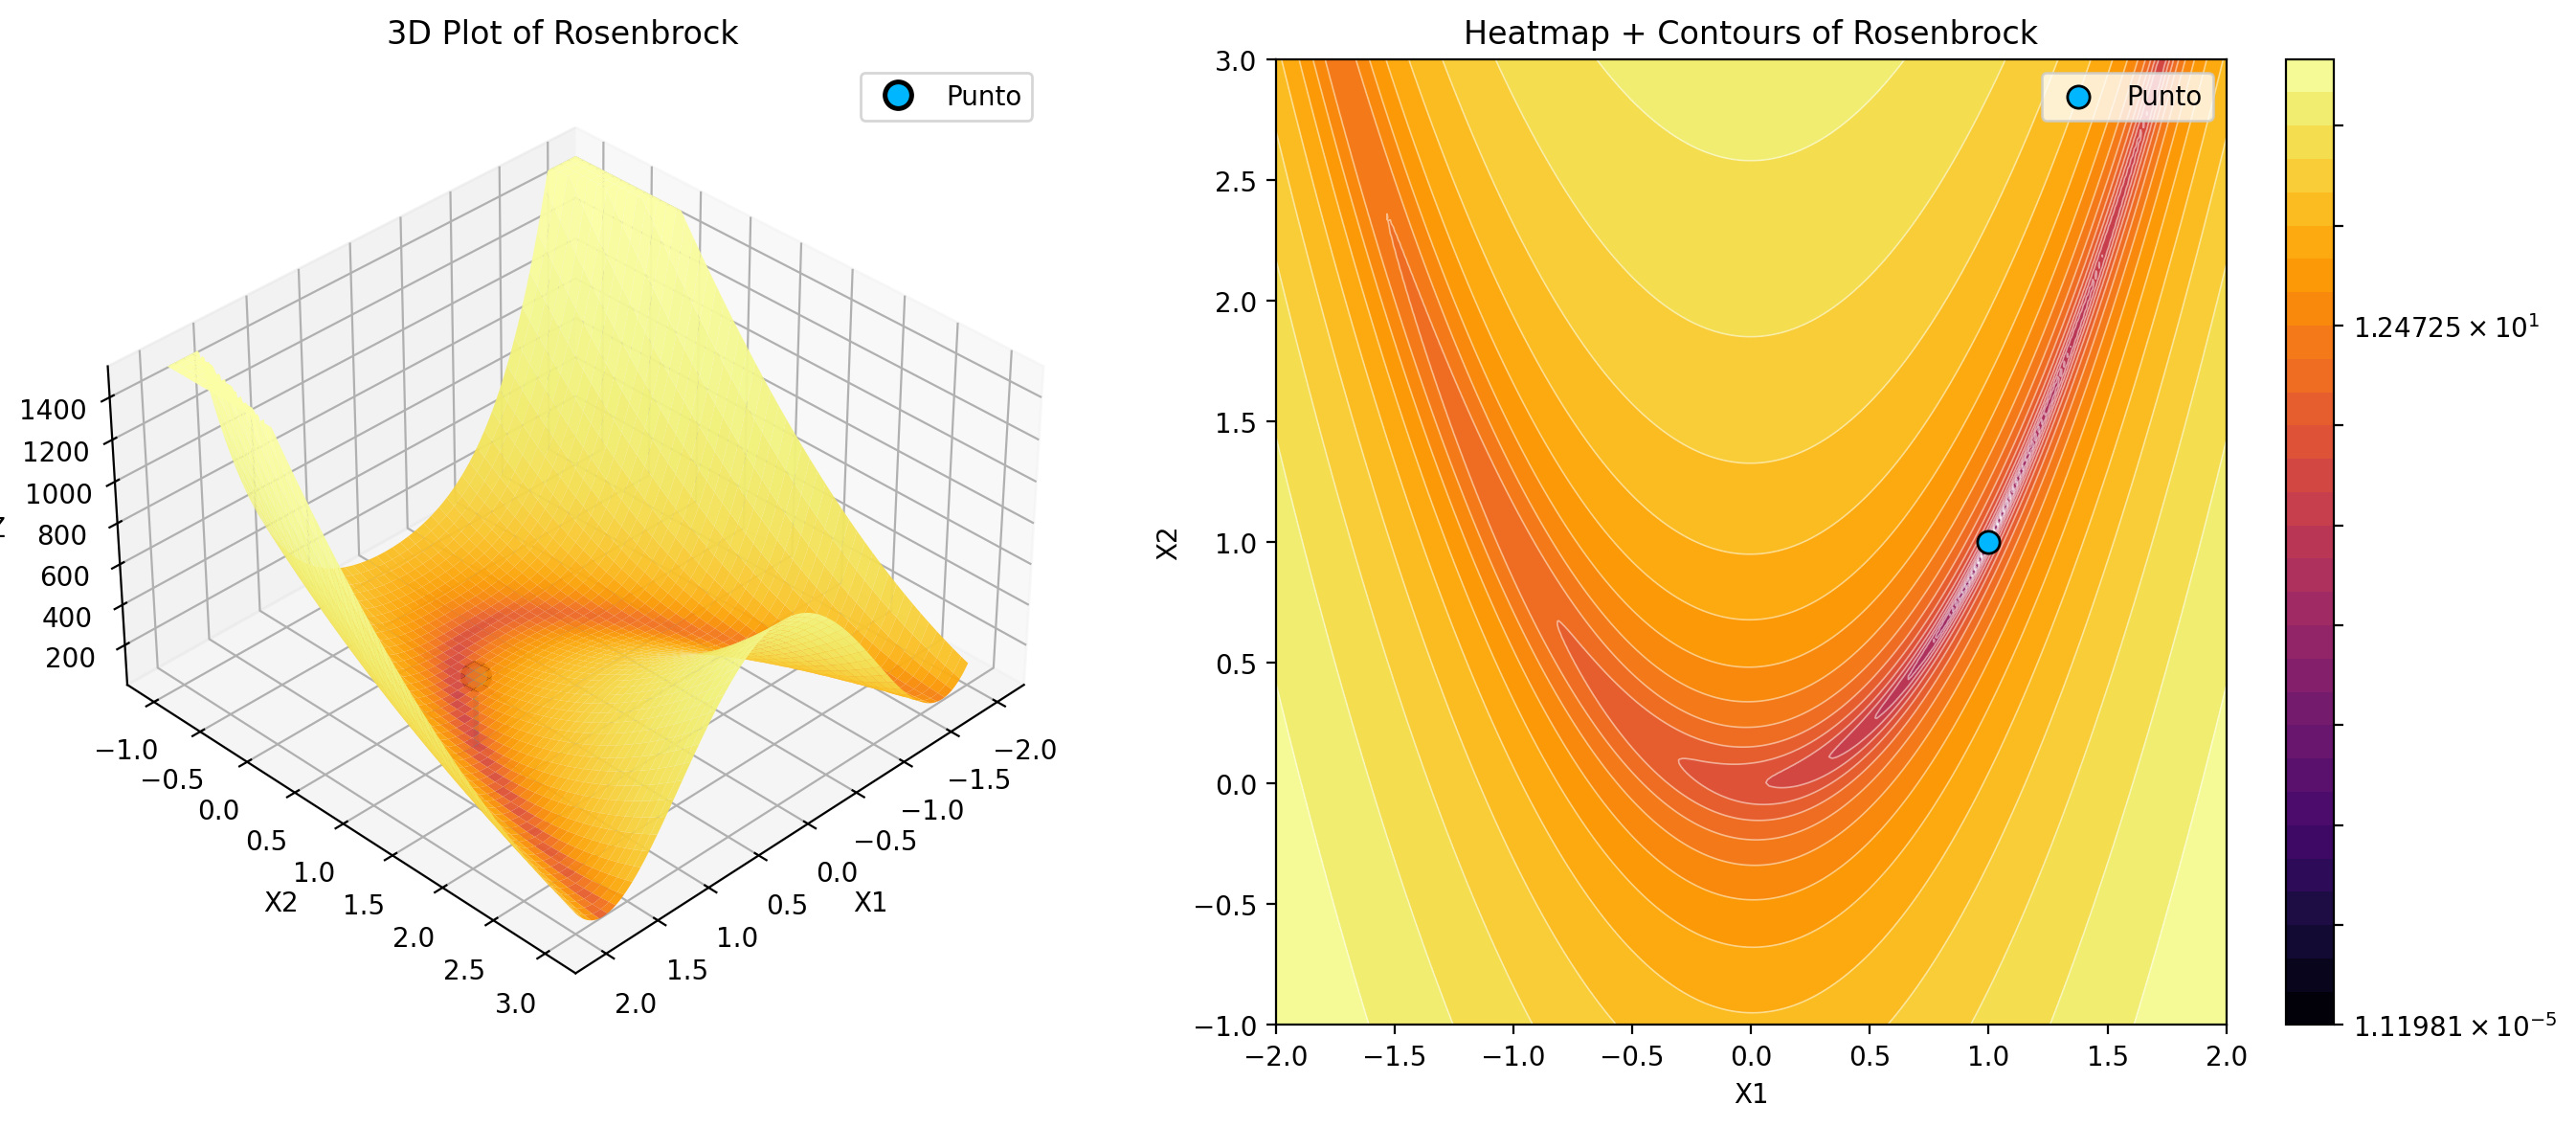
\includegraphics[keepaspectratio]{assets/numerica/gradientes/images/rosenbrock/rosenbrock_mapa_calor_y_superficie.png}}

\paragraph{Rastrigin}\label{rastrigin}

{\def\LTcaptype{none} % do not increment counter
\begin{longtable}[]{@{}
  >{\raggedright\arraybackslash}p{(\linewidth - 2\tabcolsep) * \real{0.5000}}
  >{\raggedright\arraybackslash}p{(\linewidth - 2\tabcolsep) * \real{0.5000}}@{}}
\toprule\noalign{}
\begin{minipage}[b]{\linewidth}\raggedright
Gradiente en 2D
\end{minipage} & \begin{minipage}[b]{\linewidth}\raggedright
Gradiente en 3D
\end{minipage} \\
\midrule\noalign{}
\endhead
\bottomrule\noalign{}
\endlastfoot
\( \nabla f(x, y) = \begin{bmatrix} 2x + 20\pi \sin(2\pi x) \\ 2y + 20\pi \sin(2\pi y) \end{bmatrix} \)
&
\( \nabla f(x, y, z) = \begin{bmatrix} 2x + 20\pi \sin(2\pi x) \\ 2y + 20\pi \sin(2\pi y) \\ 2z + 20\pi \sin(2\pi z) \end{bmatrix} \) \\
\end{longtable}
}

\pandocbounded{
\includegraphics[keepaspectratio]{assets/numerica/gradientes/images/rastrigin/rastrigin_mapa_calor_y_superficie.png}}

\paragraph{Schwefel}\label{schwefel}

{\def\LTcaptype{none} % do not increment counter
\begin{longtable}[]{@{}
  >{\raggedright\arraybackslash}p{(\linewidth - 2\tabcolsep) * \real{0.5000}}
  >{\raggedright\arraybackslash}p{(\linewidth - 2\tabcolsep) * \real{0.5000}}@{}}
\toprule\noalign{}
\begin{minipage}[b]{\linewidth}\raggedright
Gradiente en 2D
\end{minipage} & \begin{minipage}[b]{\linewidth}\raggedright
Gradiente en 3D
\end{minipage} \\
\midrule\noalign{}
\endhead
\bottomrule\noalign{}
\endlastfoot
\( \nabla f(x, y) = \begin{bmatrix} -\sin\left(\sqrt{|x|}\right) - \frac{x \cos\left(\sqrt{|x|}\right)}{2\sqrt{|x|}} \\ -\sin\left(\sqrt{|y|}\right) - \frac{y \cos\left(\sqrt{|y|}\right)}{2\sqrt{|y|}} \end{bmatrix} \)
&
\( \nabla f(x, y, z) = \begin{bmatrix} -\sin\left(\sqrt{|x|}\right) - \frac{x \cos\left(\sqrt{|x|}\right)}{2\sqrt{|x|}} \\ -\sin\left(\sqrt{|y|}\right) - \frac{y \cos\left(\sqrt{|y|}\right)}{2\sqrt{|y|}} \\ -\sin\left(\sqrt{|z|}\right) - \frac{z \cos\left(\sqrt{|z|}\right)}{2\sqrt{|z|}} \end{bmatrix} \) \\
\end{longtable}
}

\pandocbounded{
\includegraphics[keepaspectratio]{assets/numerica/gradientes/images/schwefel/schwefel_mapa_calor_y_superficie.png}}

\paragraph{Griewank}\label{griewank}

{\def\LTcaptype{none} % do not increment counter
\begin{longtable}[]{@{}
  >{\raggedright\arraybackslash}p{(\linewidth - 2\tabcolsep) * \real{0.5000}}
  >{\raggedright\arraybackslash}p{(\linewidth - 2\tabcolsep) * \real{0.5000}}@{}}
\toprule\noalign{}
\begin{minipage}[b]{\linewidth}\raggedright
Gradiente en 2D
\end{minipage} & \begin{minipage}[b]{\linewidth}\raggedright
Gradiente en 3D
\end{minipage} \\
\midrule\noalign{}
\endhead
\bottomrule\noalign{}
\endlastfoot
\( \nabla f(x, y) = \begin{bmatrix} \frac{x}{2000} + \frac{1}{\sqrt{1}} \sin\left(\frac{x}{\sqrt{1}}\right) \cos\left(\frac{y}{\sqrt{2}}\right) \\ \frac{y}{2000} + \frac{1}{\sqrt{2}} \cos\left(\frac{x}{\sqrt{1}}\right) \sin\left(\frac{y}{\sqrt{2}}\right) \end{bmatrix} \)
&
\( \nabla f(x, y, z) = \begin{bmatrix} \frac{x}{2000} + \frac{1}{\sqrt{1}} \sin\left(\frac{x}{\sqrt{1}}\right) \cos\left(\frac{y}{\sqrt{2}}\right) \cos\left(\frac{z}{\sqrt{3}}\right) \\ \frac{y}{2000} + \frac{1}{\sqrt{2}} \cos\left(\frac{x}{\sqrt{1}}\right) \sin\left(\frac{y}{\sqrt{2}}\right) \cos\left(\frac{z}{\sqrt{3}}\right) \\ \frac{z}{2000} + \frac{1}{\sqrt{3}} \cos\left(\frac{x}{\sqrt{1}}\right) \cos\left(\frac{y}{\sqrt{2}}\right) \sin\left(\frac{z}{\sqrt{3}}\right) \end{bmatrix} \) \\
\end{longtable}
}

\pandocbounded{
\includegraphics[keepaspectratio]{assets/numerica/gradientes/images/griewank/griewank_mapa_calor_y_superficie.png}}

\paragraph{Goldstein-Price}\label{goldstein-price}

{\def\LTcaptype{none} % do not increment counter
\begin{longtable}[]{@{}
  >{\raggedright\arraybackslash}p{(\linewidth - 0\tabcolsep) * \real{1.0000}}@{}}
\toprule\noalign{}
\begin{minipage}[b]{\linewidth}\raggedright
Gradiente en 2D
\end{minipage} \\
\midrule\noalign{}
\endhead
\bottomrule\noalign{}
\endlastfoot
\( \nabla f(x, y) = \begin{bmatrix} \frac{\partial f}{\partial x} \\ \frac{\partial f}{\partial y} \end{bmatrix} \) \\
\end{longtable}
}

\pandocbounded{
\includegraphics[keepaspectratio]{assets/numerica/gradientes/images/goldstein_price/goldstein_price_mapa_calor_y_superficie.png}}

\paragraph{Six-Hump Camel}\label{six-hump-camel}

{\def\LTcaptype{none} % do not increment counter
\begin{longtable}[]{@{}
  >{\raggedright\arraybackslash}p{(\linewidth - 0\tabcolsep) * \real{1.0000}}@{}}
\toprule\noalign{}
\begin{minipage}[b]{\linewidth}\raggedright
Gradiente en 2D
\end{minipage} \\
\midrule\noalign{}
\endhead
\bottomrule\noalign{}
\endlastfoot
\( \nabla f(x, y) = \begin{bmatrix} (8 - 8.4x^2 + 2x^4)x + y \\ x + (-8 + 16y^2)y \end{bmatrix} \) \\
\end{longtable}
}

\pandocbounded{
\includegraphics[keepaspectratio]{assets/numerica/gradientes/images/six_hump_camel/six_hump_camel_mapa_calor_y_superficie.png}}

\subsubsection{Tabla resumen de
desempeño}\label{tabla-resumen-de-desempeuxf1o}

A continuación se muestra el detalle específico de las funciones
evaluadas en ambas dimensiones, o en una sola cuando corresponde. Esto
permite observar con mayor claridad cómo cambia el desempeño del método
cuando aumenta el número de corridas y cómo se distribuyen los
resultados finales.

\paragraph{Rosenbrock}\label{rosenbrock-1}

{\def\LTcaptype{none} % do not increment counter
\begin{longtable}[]{@{}
  >{\raggedleft\arraybackslash}p{(\linewidth - 16\tabcolsep) * \real{0.1111}}
  >{\raggedleft\arraybackslash}p{(\linewidth - 16\tabcolsep) * \real{0.1111}}
  >{\raggedleft\arraybackslash}p{(\linewidth - 16\tabcolsep) * \real{0.1111}}
  >{\raggedleft\arraybackslash}p{(\linewidth - 16\tabcolsep) * \real{0.1111}}
  >{\raggedleft\arraybackslash}p{(\linewidth - 16\tabcolsep) * \real{0.1111}}
  >{\raggedleft\arraybackslash}p{(\linewidth - 16\tabcolsep) * \real{0.1111}}
  >{\raggedleft\arraybackslash}p{(\linewidth - 16\tabcolsep) * \real{0.1111}}
  >{\raggedleft\arraybackslash}p{(\linewidth - 16\tabcolsep) * \real{0.1111}}
  >{\raggedleft\arraybackslash}p{(\linewidth - 16\tabcolsep) * \real{0.1111}}@{}}
\toprule\noalign{}
\begin{minipage}[b]{\linewidth}\raggedleft
Dimensión
\end{minipage} & \begin{minipage}[b]{\linewidth}\raggedleft
Corridas
\end{minipage} & \begin{minipage}[b]{\linewidth}\raggedleft
Mejor valor final
\end{minipage} & \begin{minipage}[b]{\linewidth}\raggedleft
Peor valor final
\end{minipage} & \begin{minipage}[b]{\linewidth}\raggedleft
Promedio del valor final
\end{minipage} & \begin{minipage}[b]{\linewidth}\raggedleft
Mediana del valor final
\end{minipage} & \begin{minipage}[b]{\linewidth}\raggedleft
Desv. del valor final
\end{minipage} & \begin{minipage}[b]{\linewidth}\raggedleft
Promedio de evaluaciones
\end{minipage} & \begin{minipage}[b]{\linewidth}\raggedleft
Promedio de iteraciones
\end{minipage} \\
\midrule\noalign{}
\endhead
\bottomrule\noalign{}
\endlastfoot
2D & 100 & 0.00 & 5.20 & 2.27 & 1.86 & 1.71 & 1002.00 & 1000.00 \\
2D & 500 & 0.00 & 5.65 & 1.49 & 0.75 & 1.65 & 1002.00 & 1000.00 \\
2D & 1000 & 0.00 & 5.65 & 1.49 & 0.75 & 1.59 & 1002.00 & 1000.00 \\
3D & 100 & 0.09 & 4.32 & 2.26 & 2.59 & 1.10 & 1002.00 & 1000.00 \\
3D & 500 & 0.09 & 4.79 & 2.02 & 1.87 & 1.17 & 1002.00 & 1000.00 \\
3D & 1000 & 0.03 & 4.79 & 2.03 & 2.18 & 1.17 & 1002.00 & 1000.00 \\
\end{longtable}
}

Se evidencia que encuentra soluciones muy cercanas al óptimo en 2D, pero
el valle estrecho y el acoplamiento en 3D dificultan ligeramente el
desempeño promedio.

\paragraph{Rastrigin}\label{rastrigin-1}

{\def\LTcaptype{none} % do not increment counter
\begin{longtable}[]{@{}
  >{\raggedleft\arraybackslash}p{(\linewidth - 16\tabcolsep) * \real{0.1111}}
  >{\raggedleft\arraybackslash}p{(\linewidth - 16\tabcolsep) * \real{0.1111}}
  >{\raggedleft\arraybackslash}p{(\linewidth - 16\tabcolsep) * \real{0.1111}}
  >{\raggedleft\arraybackslash}p{(\linewidth - 16\tabcolsep) * \real{0.1111}}
  >{\raggedleft\arraybackslash}p{(\linewidth - 16\tabcolsep) * \real{0.1111}}
  >{\raggedleft\arraybackslash}p{(\linewidth - 16\tabcolsep) * \real{0.1111}}
  >{\raggedleft\arraybackslash}p{(\linewidth - 16\tabcolsep) * \real{0.1111}}
  >{\raggedleft\arraybackslash}p{(\linewidth - 16\tabcolsep) * \real{0.1111}}
  >{\raggedleft\arraybackslash}p{(\linewidth - 16\tabcolsep) * \real{0.1111}}@{}}
\toprule\noalign{}
\begin{minipage}[b]{\linewidth}\raggedleft
Dimensión
\end{minipage} & \begin{minipage}[b]{\linewidth}\raggedleft
Corridas
\end{minipage} & \begin{minipage}[b]{\linewidth}\raggedleft
Mejor valor final
\end{minipage} & \begin{minipage}[b]{\linewidth}\raggedleft
Peor valor final
\end{minipage} & \begin{minipage}[b]{\linewidth}\raggedleft
Promedio del valor final
\end{minipage} & \begin{minipage}[b]{\linewidth}\raggedleft
Mediana del valor final
\end{minipage} & \begin{minipage}[b]{\linewidth}\raggedleft
Desv. del valor final
\end{minipage} & \begin{minipage}[b]{\linewidth}\raggedleft
Promedio de evaluaciones
\end{minipage} & \begin{minipage}[b]{\linewidth}\raggedleft
Promedio de iteraciones
\end{minipage} \\
\midrule\noalign{}
\endhead
\bottomrule\noalign{}
\endlastfoot
2D & 100 & 1.99 & 40.79 & 22.45 & 24.87 & 10.33 & 29.04 & 27.04 \\
2D & 500 & 0.99 & 40.79 & 17.04 & 16.91 & 10.54 & 28.85 & 26.85 \\
2D & 1000 & 0.99 & 40.79 & 16.48 & 16.91 & 10.58 & 29.05 & 27.05 \\
3D & 100 & 1.99 & 58.70 & 31.95 & 35.32 & 13.04 & 30.10 & 28.10 \\
3D & 500 & 1.99 & 58.70 & 22.71 & 21.39 & 12.31 & 31.92 & 29.92 \\
3D & 1000 & 0.99 & 58.70 & 21.55 & 20.89 & 11.74 & 32.04 & 30.04 \\
\end{longtable}
}

Se observa que sufre severamente debido a sus múltiples mínimos locales;
converge rápido pero se evidencia que queda atrapado casi de inmediato.

\paragraph{Schwefel}\label{schwefel-1}

{\def\LTcaptype{none} % do not increment counter
\begin{longtable}[]{@{}
  >{\raggedleft\arraybackslash}p{(\linewidth - 16\tabcolsep) * \real{0.1111}}
  >{\raggedleft\arraybackslash}p{(\linewidth - 16\tabcolsep) * \real{0.1111}}
  >{\raggedleft\arraybackslash}p{(\linewidth - 16\tabcolsep) * \real{0.1111}}
  >{\raggedleft\arraybackslash}p{(\linewidth - 16\tabcolsep) * \real{0.1111}}
  >{\raggedleft\arraybackslash}p{(\linewidth - 16\tabcolsep) * \real{0.1111}}
  >{\raggedleft\arraybackslash}p{(\linewidth - 16\tabcolsep) * \real{0.1111}}
  >{\raggedleft\arraybackslash}p{(\linewidth - 16\tabcolsep) * \real{0.1111}}
  >{\raggedleft\arraybackslash}p{(\linewidth - 16\tabcolsep) * \real{0.1111}}
  >{\raggedleft\arraybackslash}p{(\linewidth - 16\tabcolsep) * \real{0.1111}}@{}}
\toprule\noalign{}
\begin{minipage}[b]{\linewidth}\raggedleft
Dimensión
\end{minipage} & \begin{minipage}[b]{\linewidth}\raggedleft
Corridas
\end{minipage} & \begin{minipage}[b]{\linewidth}\raggedleft
Mejor valor final
\end{minipage} & \begin{minipage}[b]{\linewidth}\raggedleft
Peor valor final
\end{minipage} & \begin{minipage}[b]{\linewidth}\raggedleft
Promedio del valor final
\end{minipage} & \begin{minipage}[b]{\linewidth}\raggedleft
Mediana del valor final
\end{minipage} & \begin{minipage}[b]{\linewidth}\raggedleft
Desv. del valor final
\end{minipage} & \begin{minipage}[b]{\linewidth}\raggedleft
Promedio de evaluaciones
\end{minipage} & \begin{minipage}[b]{\linewidth}\raggedleft
Promedio de iteraciones
\end{minipage} \\
\midrule\noalign{}
\endhead
\bottomrule\noalign{}
\endlastfoot
2D & 100 & -15.32 & 985.87 & 369.84 & 416.60 & 254.49 & 10002.00 &
10000.00 \\
2D & 500 & -15.32 & 1225.63 & 430.81 & 401.60 & 317.57 & 10002.00 &
10000.00 \\
2D & 1000 & -15.32 & 1225.63 & 376.59 & 341.46 & 291.55 & 10002.00 &
10000.00 \\
3D & 100 & -7.73 & 1203.50 & 538.47 & 542.68 & 325.66 & 10002.00 &
10000.00 \\
3D & 500 & -7.73 & 1450.16 & 650.61 & 660.48 & 354.56 & 10002.00 &
10000.00 \\
3D & 1000 & -7.73 & 1450.16 & 565.92 & 517.55 & 351.71 & 10002.00 &
10000.00 \\
\end{longtable}
}

Se denota un comportamiento muy polarizado y altamente dependiente del
punto inicial; se evidencia que consume el total de las iteraciones con
una desviación estándar altísima.

\paragraph{Griewank}\label{griewank-1}

{\def\LTcaptype{none} % do not increment counter
\begin{longtable}[]{@{}
  >{\raggedleft\arraybackslash}p{(\linewidth - 16\tabcolsep) * \real{0.1111}}
  >{\raggedleft\arraybackslash}p{(\linewidth - 16\tabcolsep) * \real{0.1111}}
  >{\raggedleft\arraybackslash}p{(\linewidth - 16\tabcolsep) * \real{0.1111}}
  >{\raggedleft\arraybackslash}p{(\linewidth - 16\tabcolsep) * \real{0.1111}}
  >{\raggedleft\arraybackslash}p{(\linewidth - 16\tabcolsep) * \real{0.1111}}
  >{\raggedleft\arraybackslash}p{(\linewidth - 16\tabcolsep) * \real{0.1111}}
  >{\raggedleft\arraybackslash}p{(\linewidth - 16\tabcolsep) * \real{0.1111}}
  >{\raggedleft\arraybackslash}p{(\linewidth - 16\tabcolsep) * \real{0.1111}}
  >{\raggedleft\arraybackslash}p{(\linewidth - 16\tabcolsep) * \real{0.1111}}@{}}
\toprule\noalign{}
\begin{minipage}[b]{\linewidth}\raggedleft
Dimensión
\end{minipage} & \begin{minipage}[b]{\linewidth}\raggedleft
Corridas
\end{minipage} & \begin{minipage}[b]{\linewidth}\raggedleft
Mejor valor final
\end{minipage} & \begin{minipage}[b]{\linewidth}\raggedleft
Peor valor final
\end{minipage} & \begin{minipage}[b]{\linewidth}\raggedleft
Promedio del valor final
\end{minipage} & \begin{minipage}[b]{\linewidth}\raggedleft
Mediana del valor final
\end{minipage} & \begin{minipage}[b]{\linewidth}\raggedleft
Desv. del valor final
\end{minipage} & \begin{minipage}[b]{\linewidth}\raggedleft
Promedio de evaluaciones
\end{minipage} & \begin{minipage}[b]{\linewidth}\raggedleft
Promedio de iteraciones
\end{minipage} \\
\midrule\noalign{}
\endhead
\bottomrule\noalign{}
\endlastfoot
2D & 100 & 0.00 & 0.05 & 0.02 & 0.01 & 0.01 & 1766.94 & 1764.94 \\
2D & 500 & 0.00 & 0.05 & 0.02 & 0.03 & 0.01 & 1732.03 & 1730.03 \\
2D & 1000 & 0.00 & 0.05 & 0.02 & 0.03 & 0.01 & 1741.05 & 1739.05 \\
3D & 100 & 0.01 & 0.99 & 0.04 & 0.03 & 0.10 & 2002.00 & 2000.00 \\
3D & 500 & 0.01 & 0.99 & 0.04 & 0.03 & 0.04 & 2002.00 & 2000.00 \\
3D & 1000 & 0.01 & 0.99 & 0.03 & 0.03 & 0.03 & 2002.00 & 2000.00 \\
\end{longtable}
}

Se aprecia un desempeño sobresaliente y muy consistente; se demuestra
que su estructura global guía con éxito al gradiente hacia valores
cercanos a cero con mínima dispersión.

\paragraph{Goldstein-Price}\label{goldstein-price-1}

{\def\LTcaptype{none} % do not increment counter
\begin{longtable}[]{@{}
  >{\raggedleft\arraybackslash}p{(\linewidth - 16\tabcolsep) * \real{0.1111}}
  >{\raggedleft\arraybackslash}p{(\linewidth - 16\tabcolsep) * \real{0.1111}}
  >{\raggedleft\arraybackslash}p{(\linewidth - 16\tabcolsep) * \real{0.1111}}
  >{\raggedleft\arraybackslash}p{(\linewidth - 16\tabcolsep) * \real{0.1111}}
  >{\raggedleft\arraybackslash}p{(\linewidth - 16\tabcolsep) * \real{0.1111}}
  >{\raggedleft\arraybackslash}p{(\linewidth - 16\tabcolsep) * \real{0.1111}}
  >{\raggedleft\arraybackslash}p{(\linewidth - 16\tabcolsep) * \real{0.1111}}
  >{\raggedleft\arraybackslash}p{(\linewidth - 16\tabcolsep) * \real{0.1111}}
  >{\raggedleft\arraybackslash}p{(\linewidth - 16\tabcolsep) * \real{0.1111}}@{}}
\toprule\noalign{}
\begin{minipage}[b]{\linewidth}\raggedleft
Dimensión
\end{minipage} & \begin{minipage}[b]{\linewidth}\raggedleft
Corridas
\end{minipage} & \begin{minipage}[b]{\linewidth}\raggedleft
Mejor valor final
\end{minipage} & \begin{minipage}[b]{\linewidth}\raggedleft
Peor valor final
\end{minipage} & \begin{minipage}[b]{\linewidth}\raggedleft
Promedio del valor final
\end{minipage} & \begin{minipage}[b]{\linewidth}\raggedleft
Mediana del valor final
\end{minipage} & \begin{minipage}[b]{\linewidth}\raggedleft
Desv. del valor final
\end{minipage} & \begin{minipage}[b]{\linewidth}\raggedleft
Promedio de evaluaciones
\end{minipage} & \begin{minipage}[b]{\linewidth}\raggedleft
Promedio de iteraciones
\end{minipage} \\
\midrule\noalign{}
\endhead
\bottomrule\noalign{}
\endlastfoot
2D & 100 & 10.49 & 988.65 & 148.95 & 62.27 & 264.29 & 5002.00 &
5000.00 \\
2D & 500 & 10.49 & 989.72 & 288.42 & 80.68 & 361.56 & 5002.00 &
5000.00 \\
2D & 1000 & 10.49 & 989.72 & 328.08 & 81.16 & 382.52 & 5002.00 &
5000.00 \\
\end{longtable}
}

Se evidencia una alta inestabilidad y dependencia crítica del punto de
partida; se observa que acierta solo si cae en la cuenca de atracción
correcta, alcanzando errores cercanos a 1000.

\paragraph{Six-Hump Camel}\label{six-hump-camel-1}

{\def\LTcaptype{none} % do not increment counter
\begin{longtable}[]{@{}
  >{\raggedleft\arraybackslash}p{(\linewidth - 16\tabcolsep) * \real{0.1111}}
  >{\raggedleft\arraybackslash}p{(\linewidth - 16\tabcolsep) * \real{0.1111}}
  >{\raggedleft\arraybackslash}p{(\linewidth - 16\tabcolsep) * \real{0.1111}}
  >{\raggedleft\arraybackslash}p{(\linewidth - 16\tabcolsep) * \real{0.1111}}
  >{\raggedleft\arraybackslash}p{(\linewidth - 16\tabcolsep) * \real{0.1111}}
  >{\raggedleft\arraybackslash}p{(\linewidth - 16\tabcolsep) * \real{0.1111}}
  >{\raggedleft\arraybackslash}p{(\linewidth - 16\tabcolsep) * \real{0.1111}}
  >{\raggedleft\arraybackslash}p{(\linewidth - 16\tabcolsep) * \real{0.1111}}
  >{\raggedleft\arraybackslash}p{(\linewidth - 16\tabcolsep) * \real{0.1111}}@{}}
\toprule\noalign{}
\begin{minipage}[b]{\linewidth}\raggedleft
Dimensión
\end{minipage} & \begin{minipage}[b]{\linewidth}\raggedleft
Corridas
\end{minipage} & \begin{minipage}[b]{\linewidth}\raggedleft
Mejor valor final
\end{minipage} & \begin{minipage}[b]{\linewidth}\raggedleft
Peor valor final
\end{minipage} & \begin{minipage}[b]{\linewidth}\raggedleft
Promedio del valor final
\end{minipage} & \begin{minipage}[b]{\linewidth}\raggedleft
Mediana del valor final
\end{minipage} & \begin{minipage}[b]{\linewidth}\raggedleft
Desv. del valor final
\end{minipage} & \begin{minipage}[b]{\linewidth}\raggedleft
Promedio de evaluaciones
\end{minipage} & \begin{minipage}[b]{\linewidth}\raggedleft
Promedio de iteraciones
\end{minipage} \\
\midrule\noalign{}
\endhead
\bottomrule\noalign{}
\endlastfoot
2D & 100 & -1.03 & 2.10 & -0.45 & -1.03 & 1.08 & 989.10 & 987.10 \\
2D & 500 & -1.03 & 2.10 & -0.14 & -1.03 & 1.34 & 996.39 & 994.39 \\
2D & 1000 & -1.03 & 2.10 & -0.11 & -1.03 & 1.37 & 986.34 & 984.34 \\
\end{longtable}
}

Se constata que es muy estable y exitoso; se evidencia que su mediana se
fija consistentemente en el óptimo global (\(-1.03\)) a pesar de sus
mínimos secundarios.

\subsubsection{Histogramas de valor
final}\label{histogramas-de-valor-final}

Los histogramas del valor final permiten visualizar la distribución de
las soluciones obtenidas después de todas las corridas. Esta gráfica es
especialmente importante porque muestra si el algoritmo converge
repetidamente hacia una misma región del espacio de soluciones o si, por
el contrario, termina en distintos mínimos locales según la
inicialización.

Cuando la mayor parte de los valores finales se concentra cerca del
mínimo global, se puede interpretar que el método es relativamente
estable para esa función. En cambio, cuando la distribución es amplia,
sesgada o presenta varios grupos, ello sugiere que el descenso por
gradiente es sensible al punto inicial o que la función contiene
regiones donde la búsqueda local no logra llegar siempre a la mejor
solución.

\paragraph{Rosenbrock}\label{rosenbrock-2}

\subparagraph{2D}\label{d}

\pandocbounded{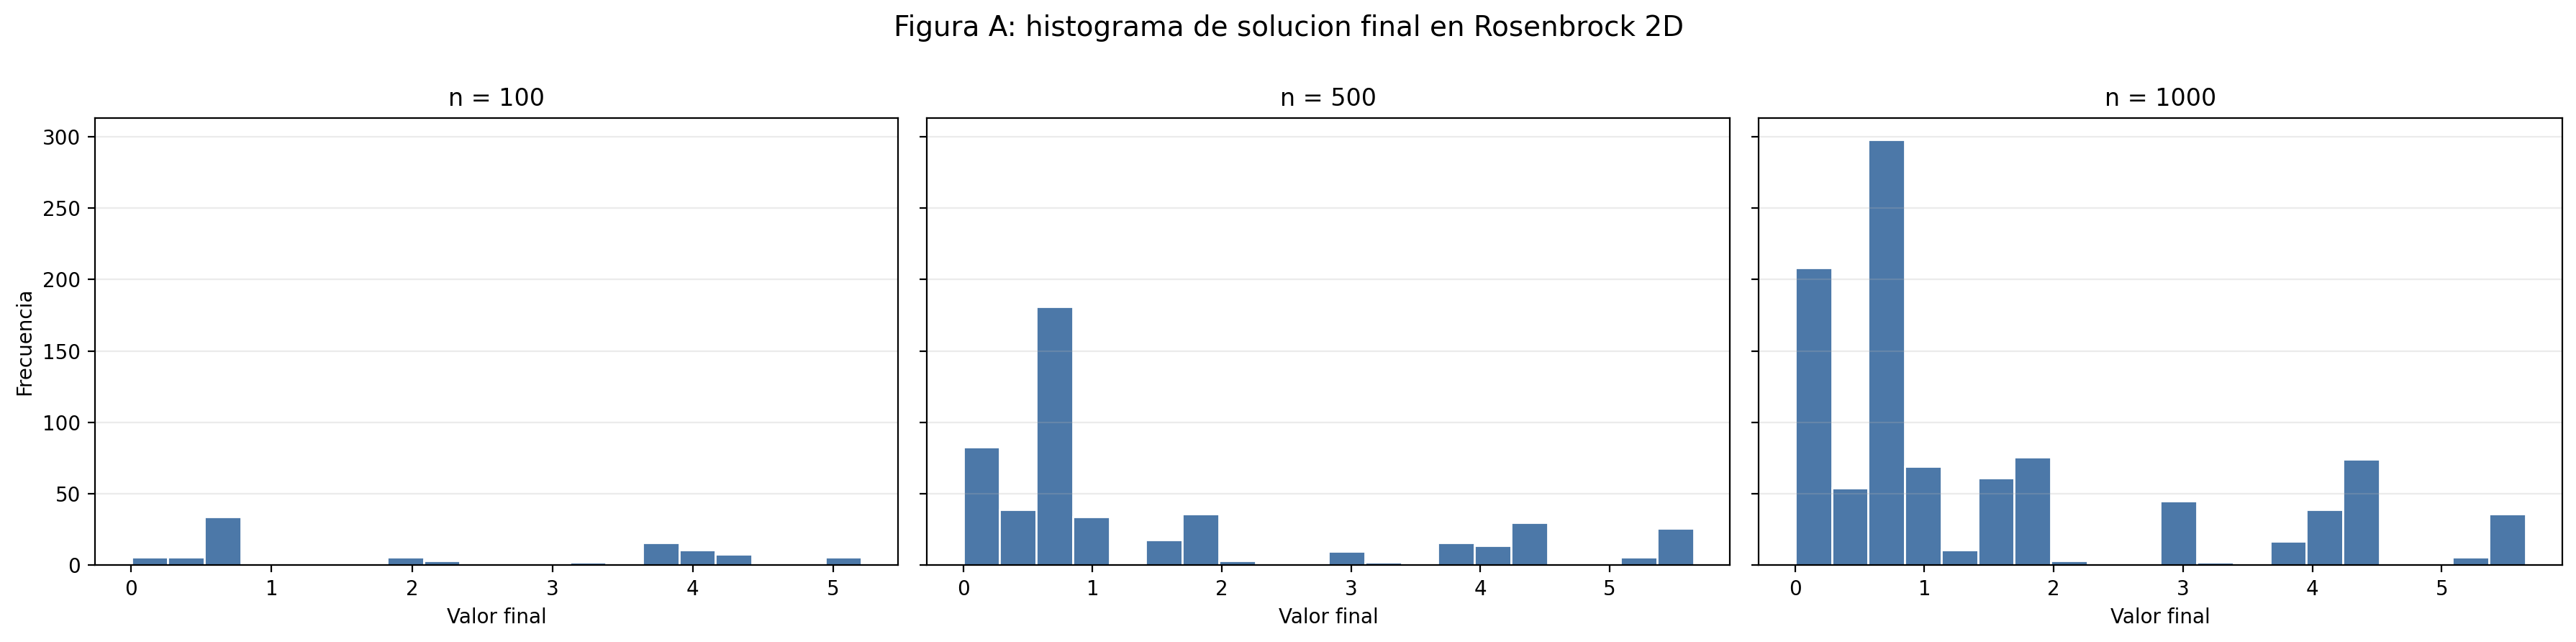
\includegraphics[keepaspectratio]{assets/numerica/gradientes/images/rosenbrock/rosenbrock_figura_a_histograma_solucion_final_2d.png}}

\subparagraph{3D}\label{d-1}

\pandocbounded{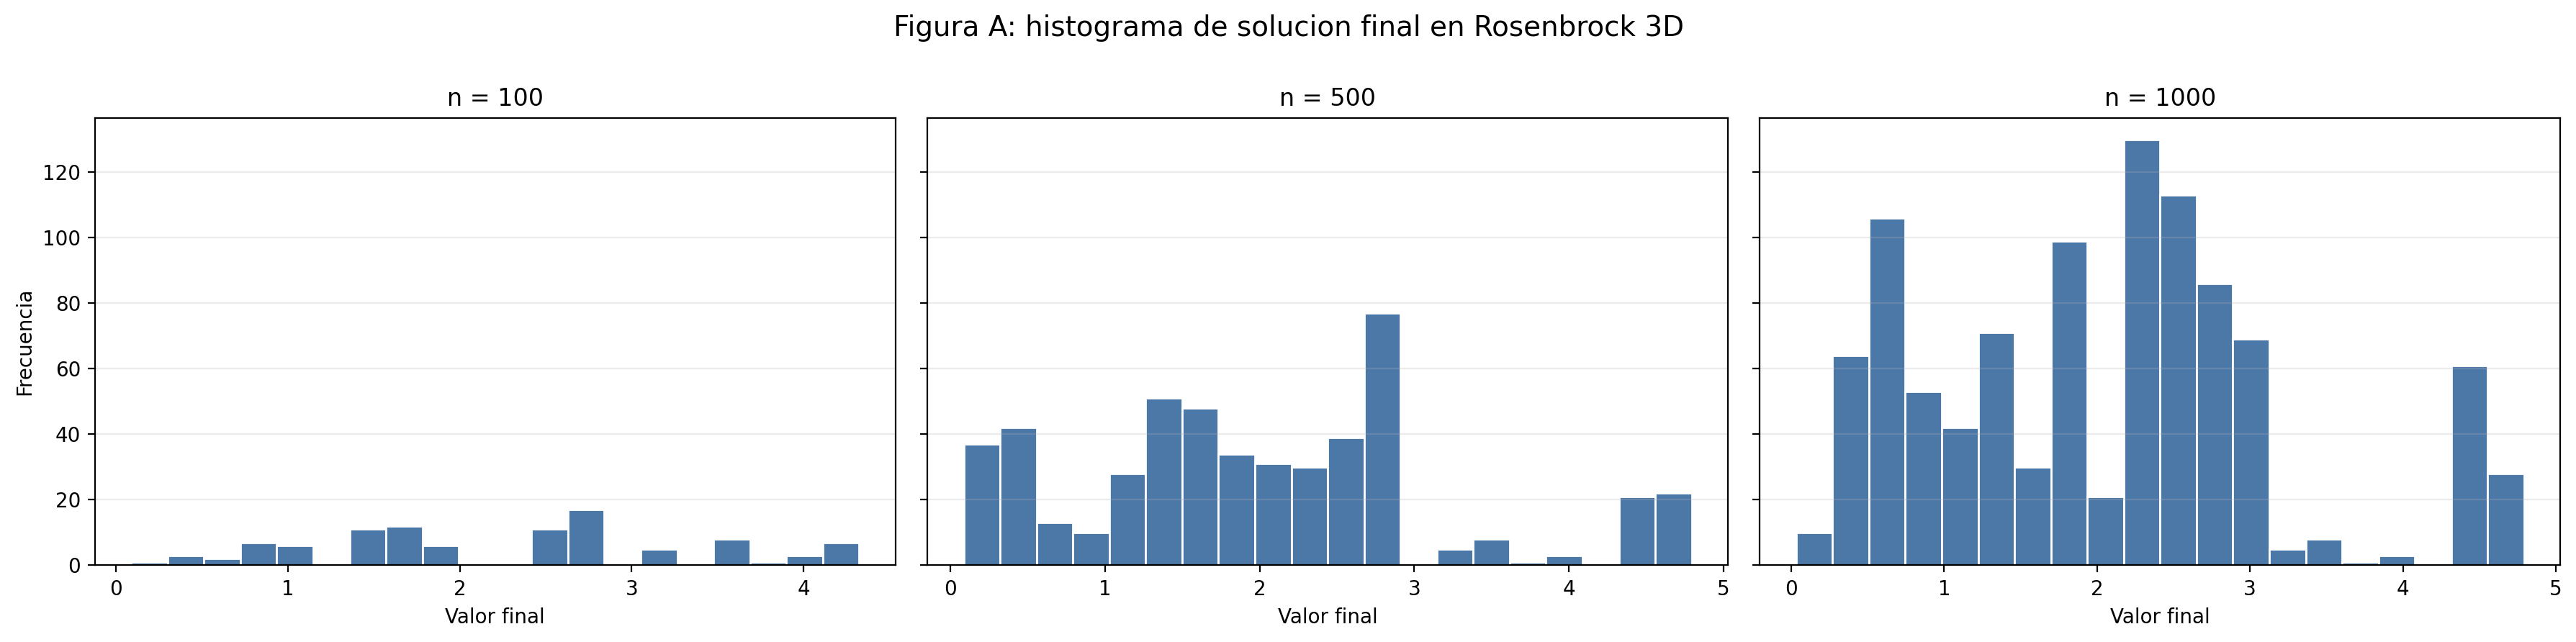
\includegraphics[keepaspectratio]{assets/numerica/gradientes/images/rosenbrock/rosenbrock_figura_a_histograma_solucion_final_3d.png}}

Se observa que en \textbf{Rosenbrock 2D}, los histogramas muestran una
fuerte concentración de frecuencias en los valores cercanos a cero
(especialmente a medida que aumentan las corridas \(n = 500\) y
\(n = 1000\)), lo que evidencia que el algoritmo logra converger
exitosamente en repetidas ocasiones hacia la región del óptimo global,
aunque persisten algunos valores dispersos debido a la dificultad de su
valle parabólico. Por otro lado, en \textbf{Rosenbrock 3D}, se denota
que la distribución se dispersa significativamente a lo largo del eje de
valores finales y aparecen múltiples grupos de frecuencias separadas;
esto evidencia que el incremento dimensional amplifica la sensibilidad
al punto inicial, provocando que el descenso por gradiente termine con
mayor frecuencia en distintas regiones o sub-óptimos locales en lugar de
consolidarse en una única zona de convergencia.

\paragraph{Rastrigin}\label{rastrigin-2}

\subparagraph{2D}\label{d-2}

\pandocbounded{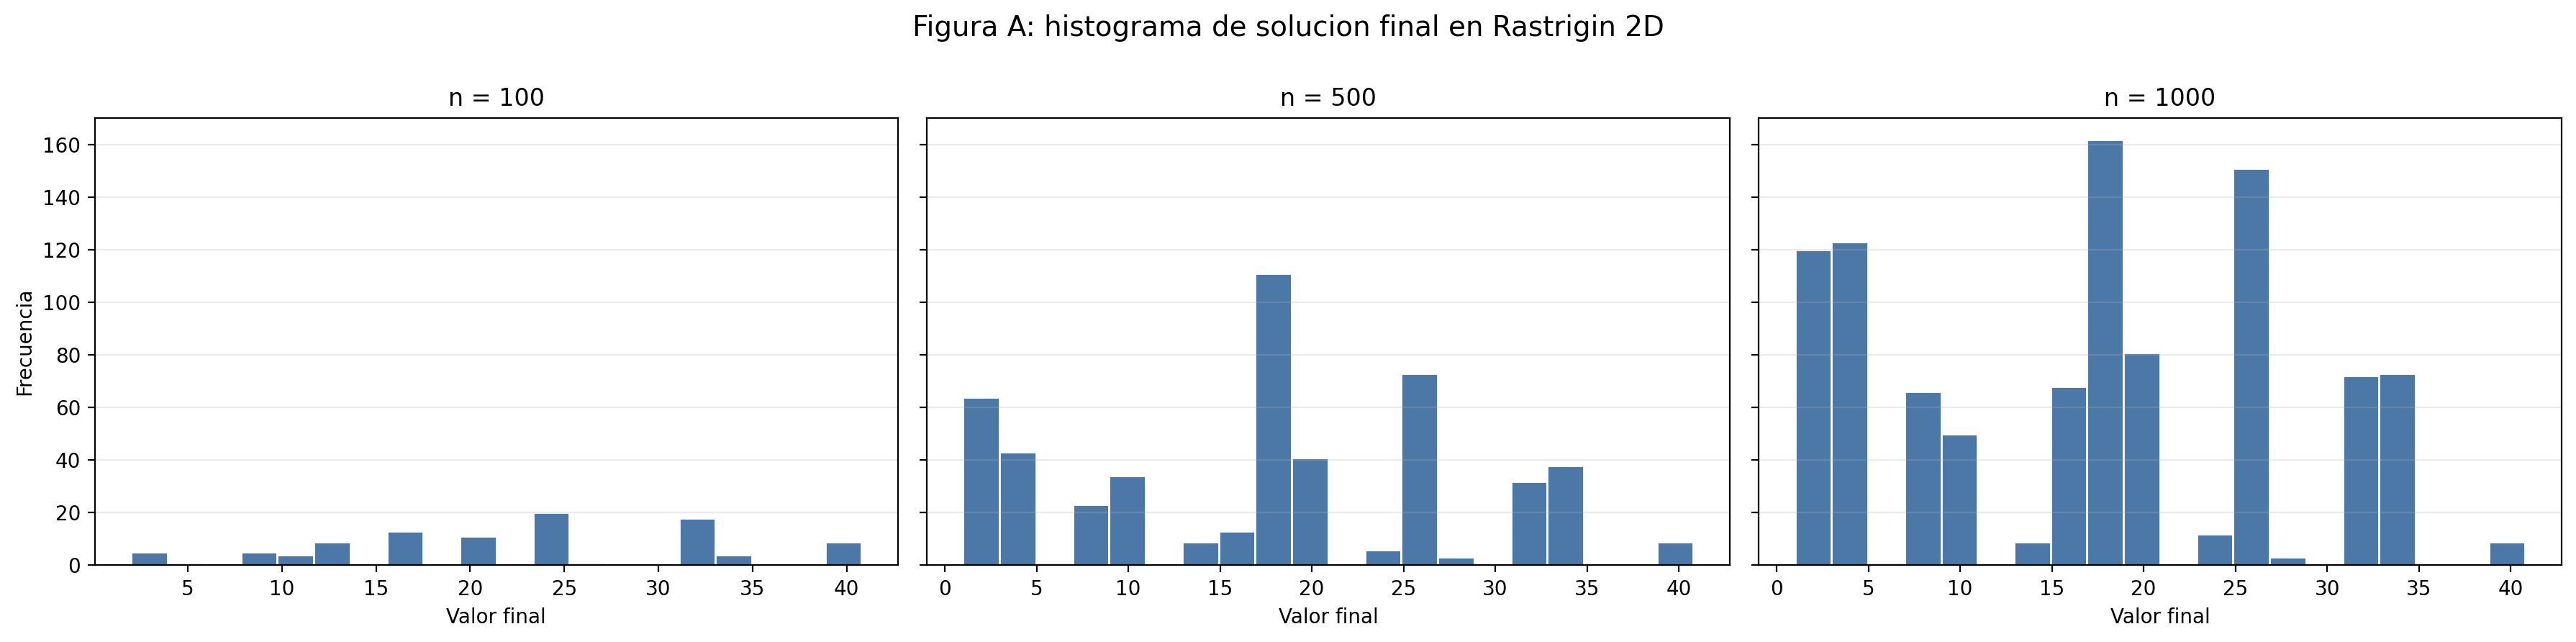
\includegraphics[keepaspectratio]{assets/numerica/gradientes/images/rastrigin/rastrigin_figura_a_histograma_solucion_final_2d.png}}

\subparagraph{3D}\label{d-3}

\pandocbounded{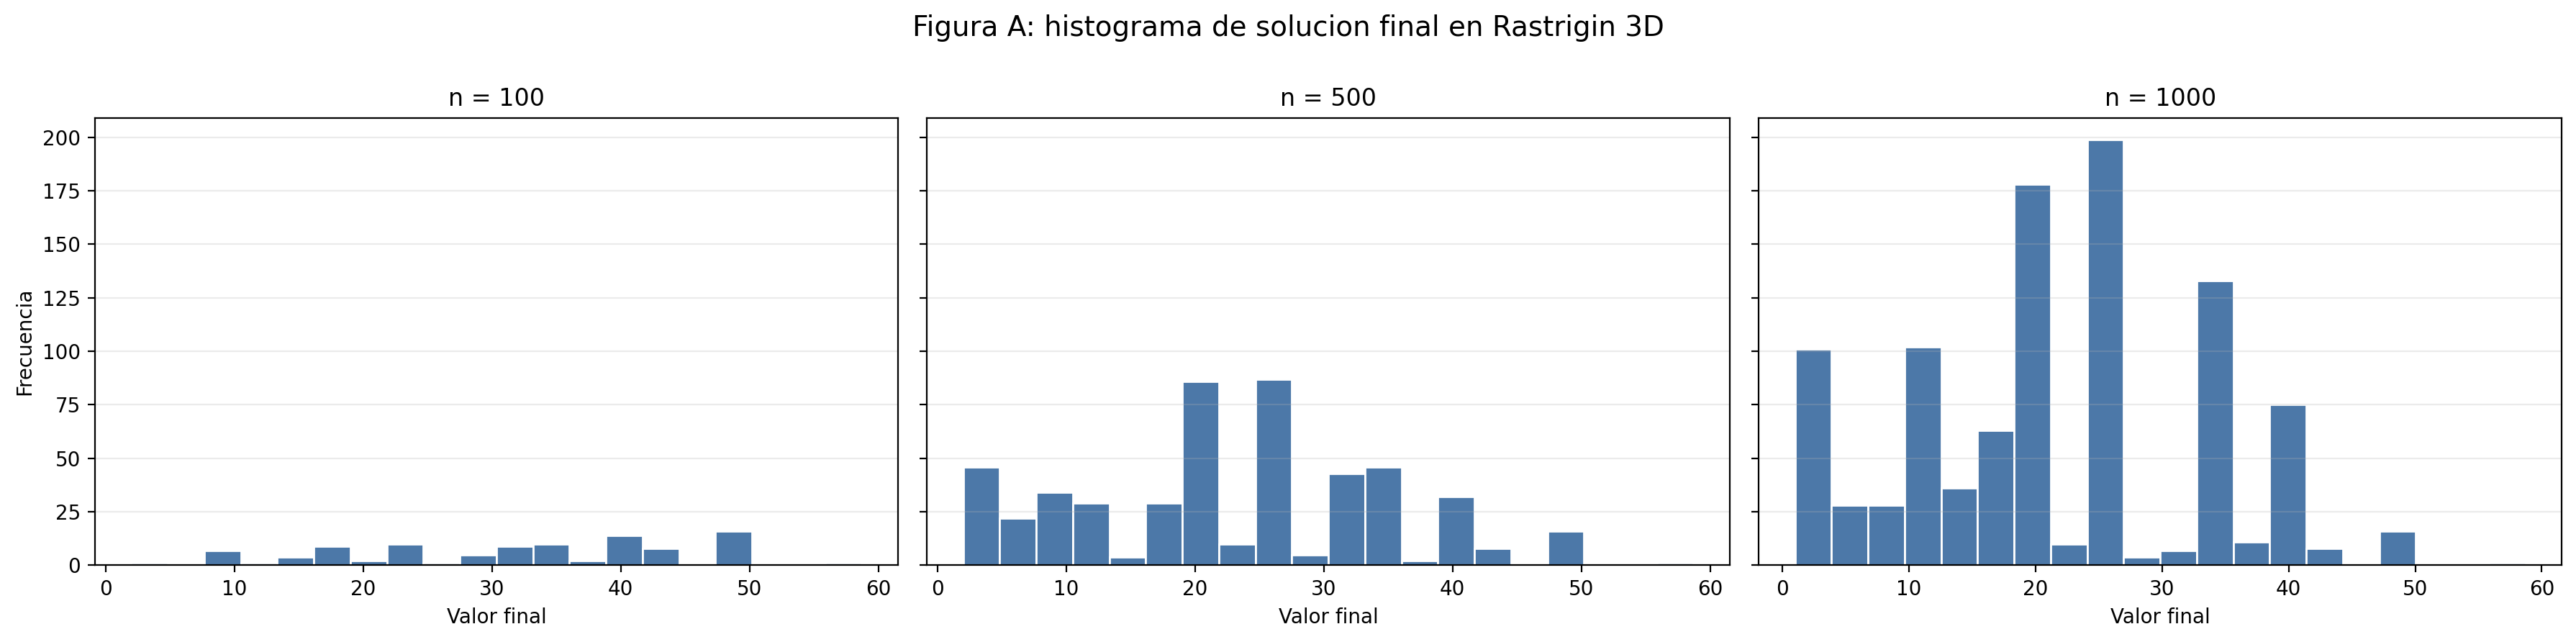
\includegraphics[keepaspectratio]{assets/numerica/gradientes/images/rastrigin/rastrigin_figura_a_histograma_solucion_final_3d.png}}

Se observa que en \textbf{Rastrigin 2D}, los histogramas muestran
múltiples grupos de frecuencia distribuidos en diversos rangos de
valores finales (con picos notables alrededor de los rangos de 0-5 y
15-20), lo que evidencia que el algoritmo es altamente sensible a la
inicialización y se estanca frecuentemente en diferentes mínimos
locales. Por su parte, en \textbf{Rastrigin 3D}, se denota que la
distribución se amplía y desplaza hacia valores finales más altos,
dispersando las frecuencias a lo largo de un espectro más amplio; esto
evidencia que el aumento de dimensionalidad incrementa exponencialmente
la cantidad de trampas multimodales, dificultando que el descenso por
gradiente converja de manera consistente hacia el óptimo global.

\paragraph{Schwefel}\label{schwefel-2}

\subparagraph{2D}\label{d-4}

\pandocbounded{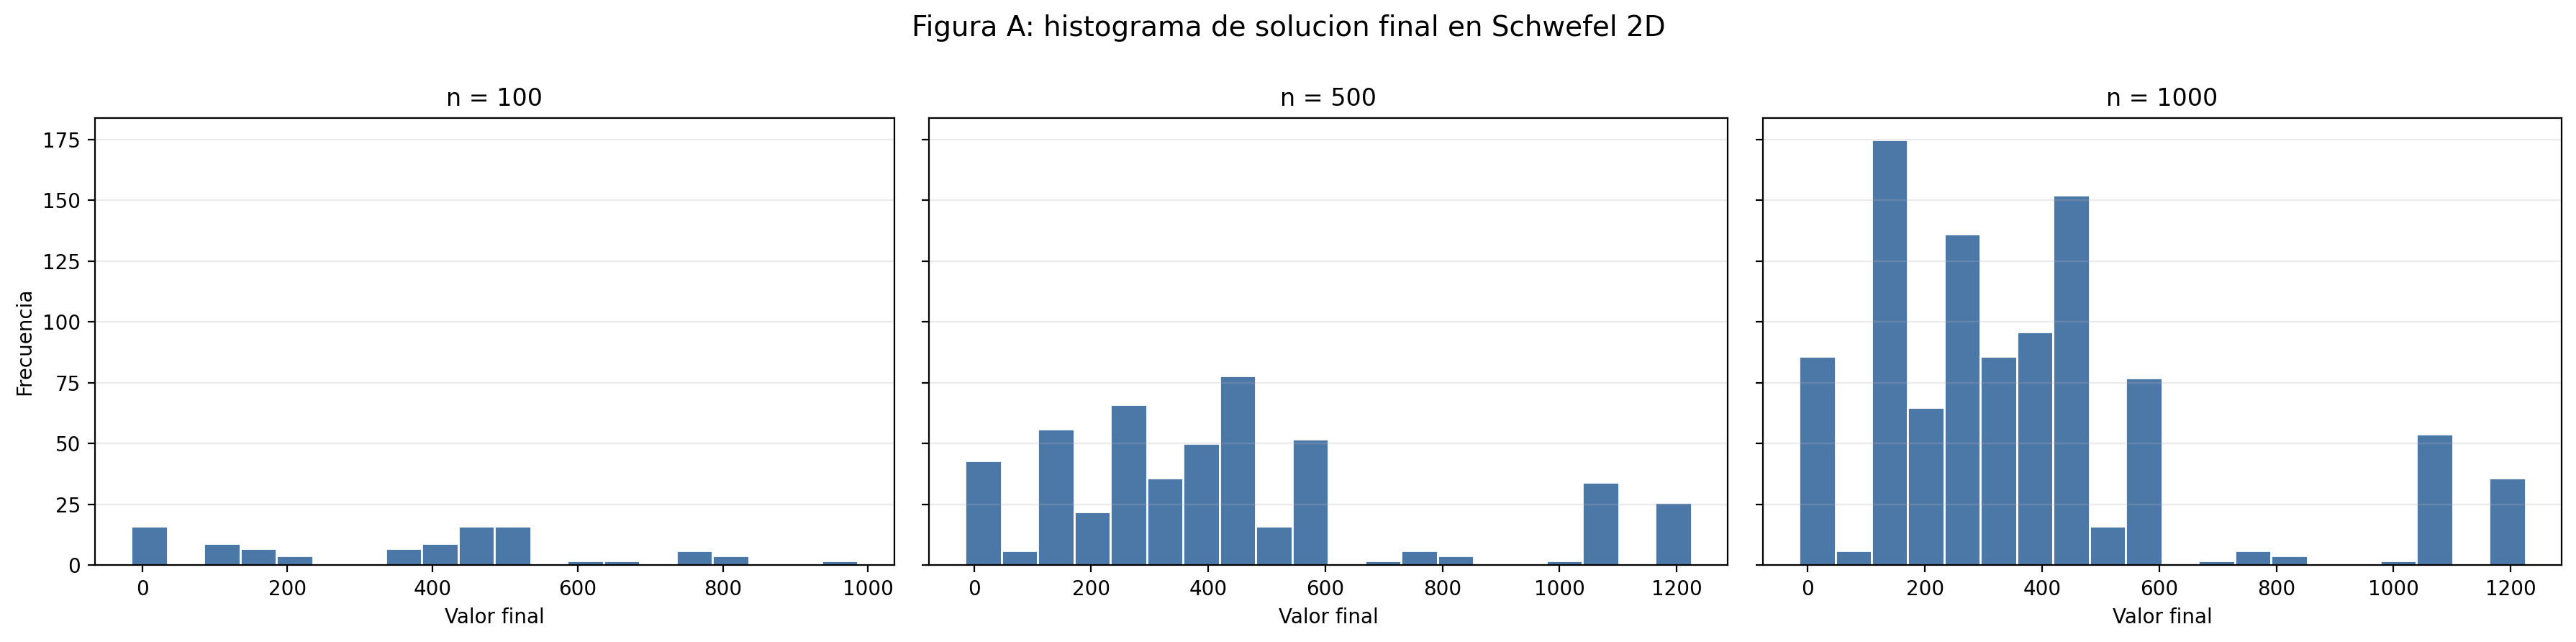
\includegraphics[keepaspectratio]{assets/numerica/gradientes/images/schwefel/schwefel_figura_a_histograma_solucion_final_2d.png}}

\subparagraph{3D}\label{d-5}

\pandocbounded{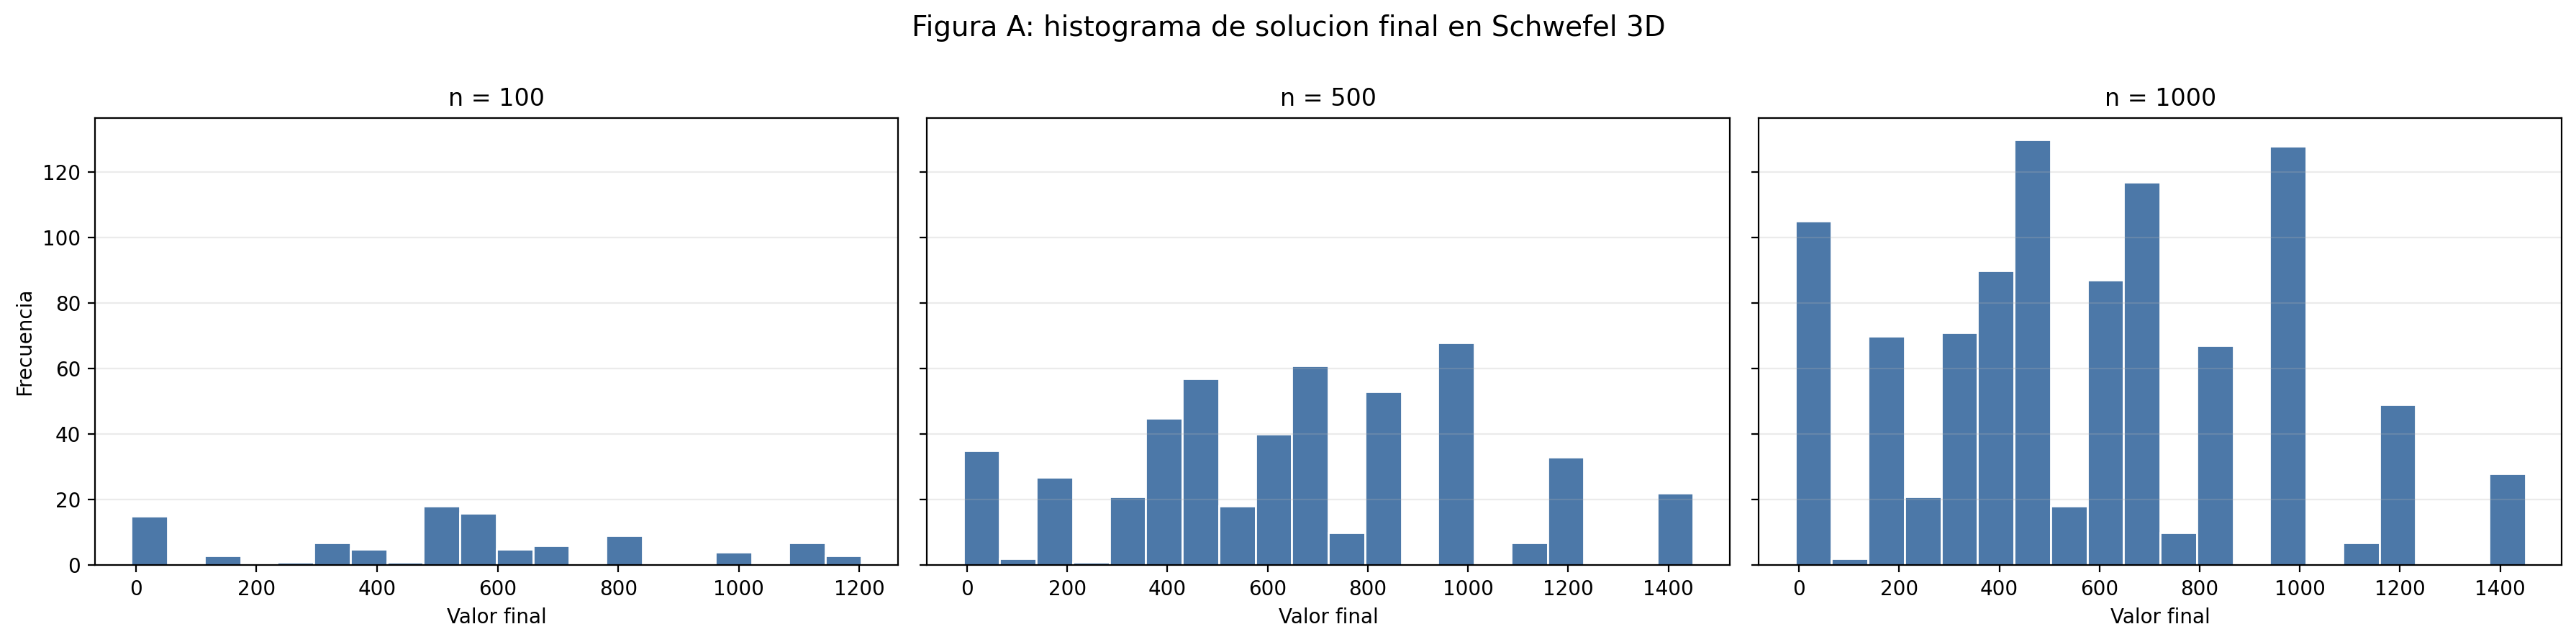
\includegraphics[keepaspectratio]{assets/numerica/gradientes/images/schwefel/schwefel_figura_a_histograma_solucion_final_3d.png}}

Se observa que en \textbf{Schwefel 2D}, los histogramas muestran una
dispersión muy amplia de las frecuencias a lo largo de un gran rango de
valores finales (con concentraciones intermedias y altas cifras que
superan los 1000), lo que evidencia que el algoritmo es sumamente
inestable y depende críticamente del punto de inicialización. Por otro
lado, en \textbf{Schwefel 3D}, se denota que la distribución se desplaza
aún más hacia la derecha y amplía su dispersión alcanzando valores
finales cercanos a 1400; esto evidencia que la severa complejidad de su
paisaje sinusoidal y el incremento dimensional provocan que el descenso
por gradiente quede atrapado de forma masiva en mínimos locales pobres
en lugar de hallar el óptimo global.

\paragraph{Griewank}\label{griewank-2}

\subparagraph{2D}\label{d-6}

\pandocbounded{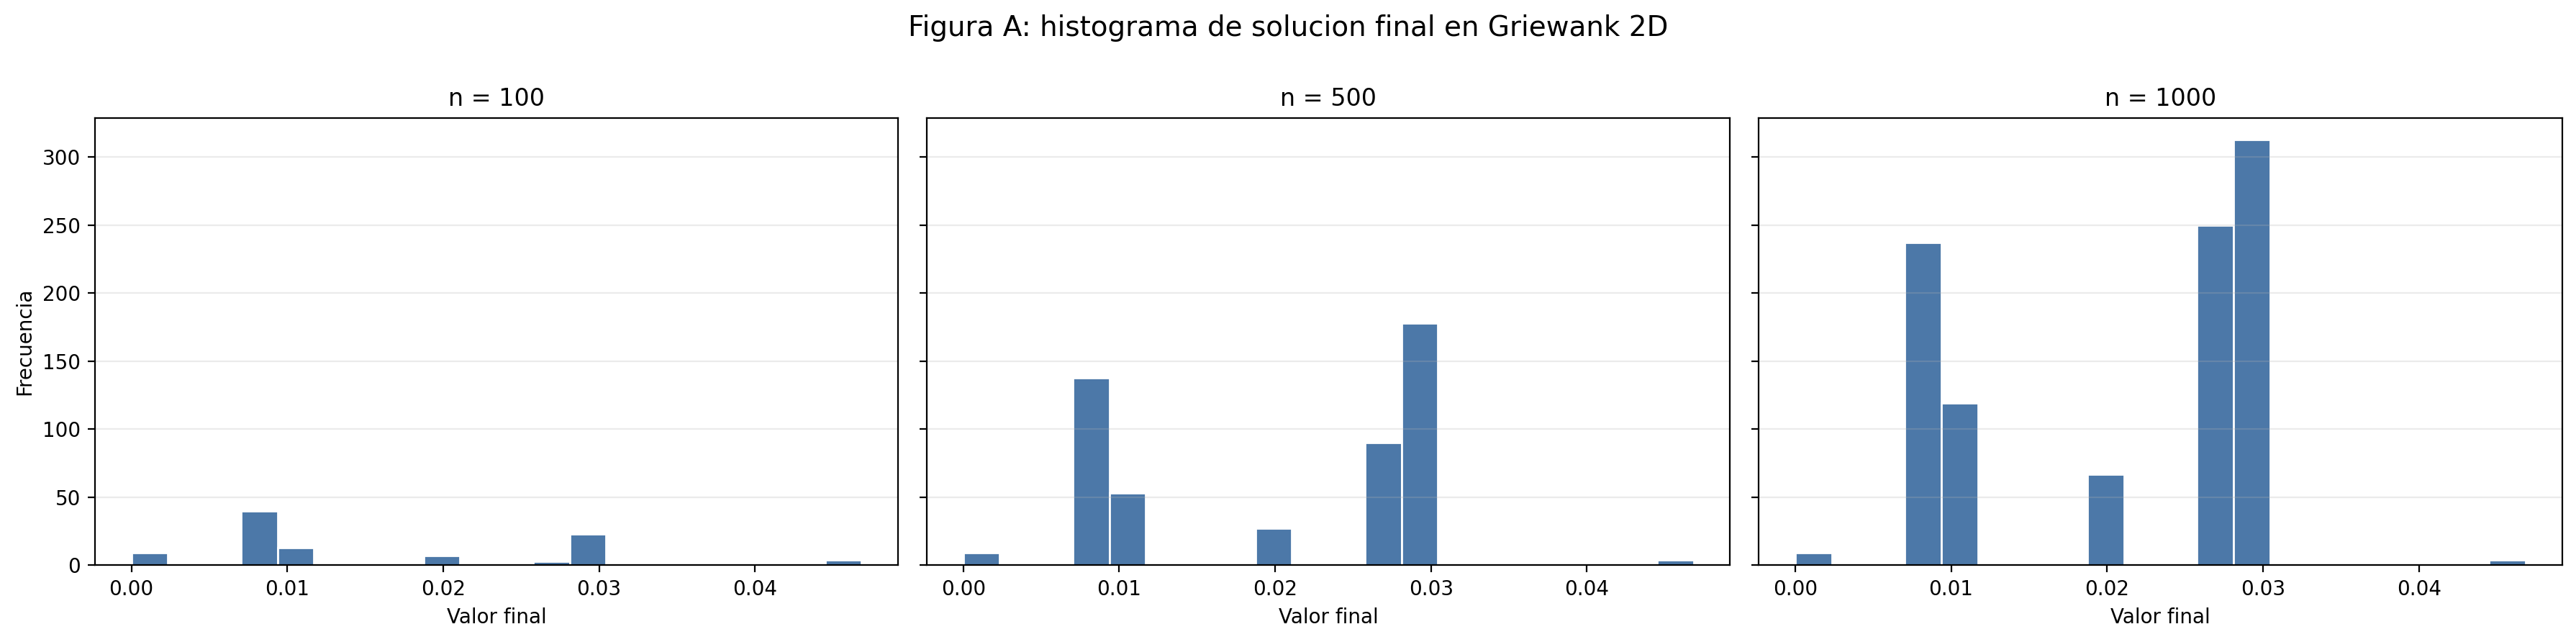
\includegraphics[keepaspectratio]{assets/numerica/gradientes/images/griewank/griewank_figura_a_histograma_solucion_final_2d.png}}

\subparagraph{3D}\label{d-7}

\pandocbounded{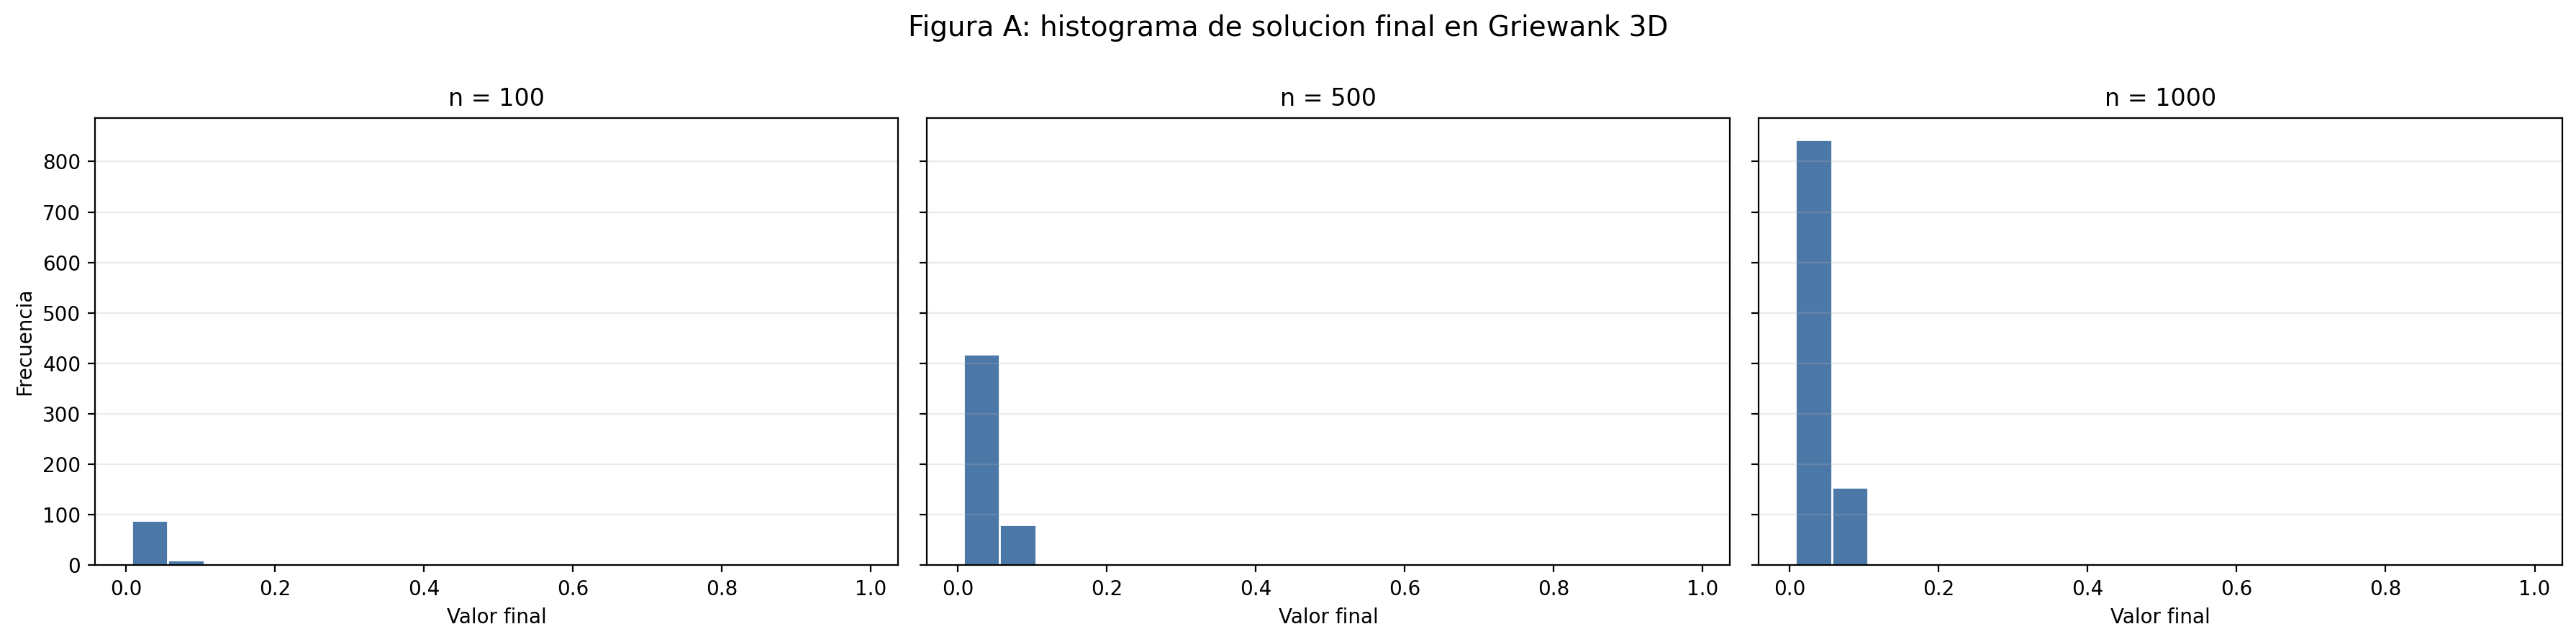
\includegraphics[keepaspectratio]{assets/numerica/gradientes/images/griewank/griewank_figura_a_histograma_solucion_final_3d.png}}

Se observa que en \textbf{Griewank 2D}, los histogramas muestran una
concentración de frecuencias muy estrecha y compacta en valores
extremadamente cercanos a cero (con un rango limitado que apenas alcanza
los 0.05), lo que evidencia que el algoritmo posee una excelente
consistencia y estabilidad para converger repetidamente cerca del óptimo
global. Por otro lado, en \textbf{Griewank 3D}, se denota que las
frecuencias se concentran fuertemente en el primer tramo inferior
cercano a cero (con picos muy altos en las corridas de \(n = 500\) y
\(n = 1000\)), aunque con una ligera dispersión que se extiende hacia
valores cercanos a 1.0; esto evidencia que, a pesar de un leve
incremento en la variabilidad debido a la dimensión, la estructura
global de la función permite que el descenso por gradiente mantenga una
alta efectividad y robustez en la búsqueda de la solución.

\paragraph{Goldstein-Price}\label{goldstein-price-2}

\subparagraph{2D}\label{d-8}

\pandocbounded{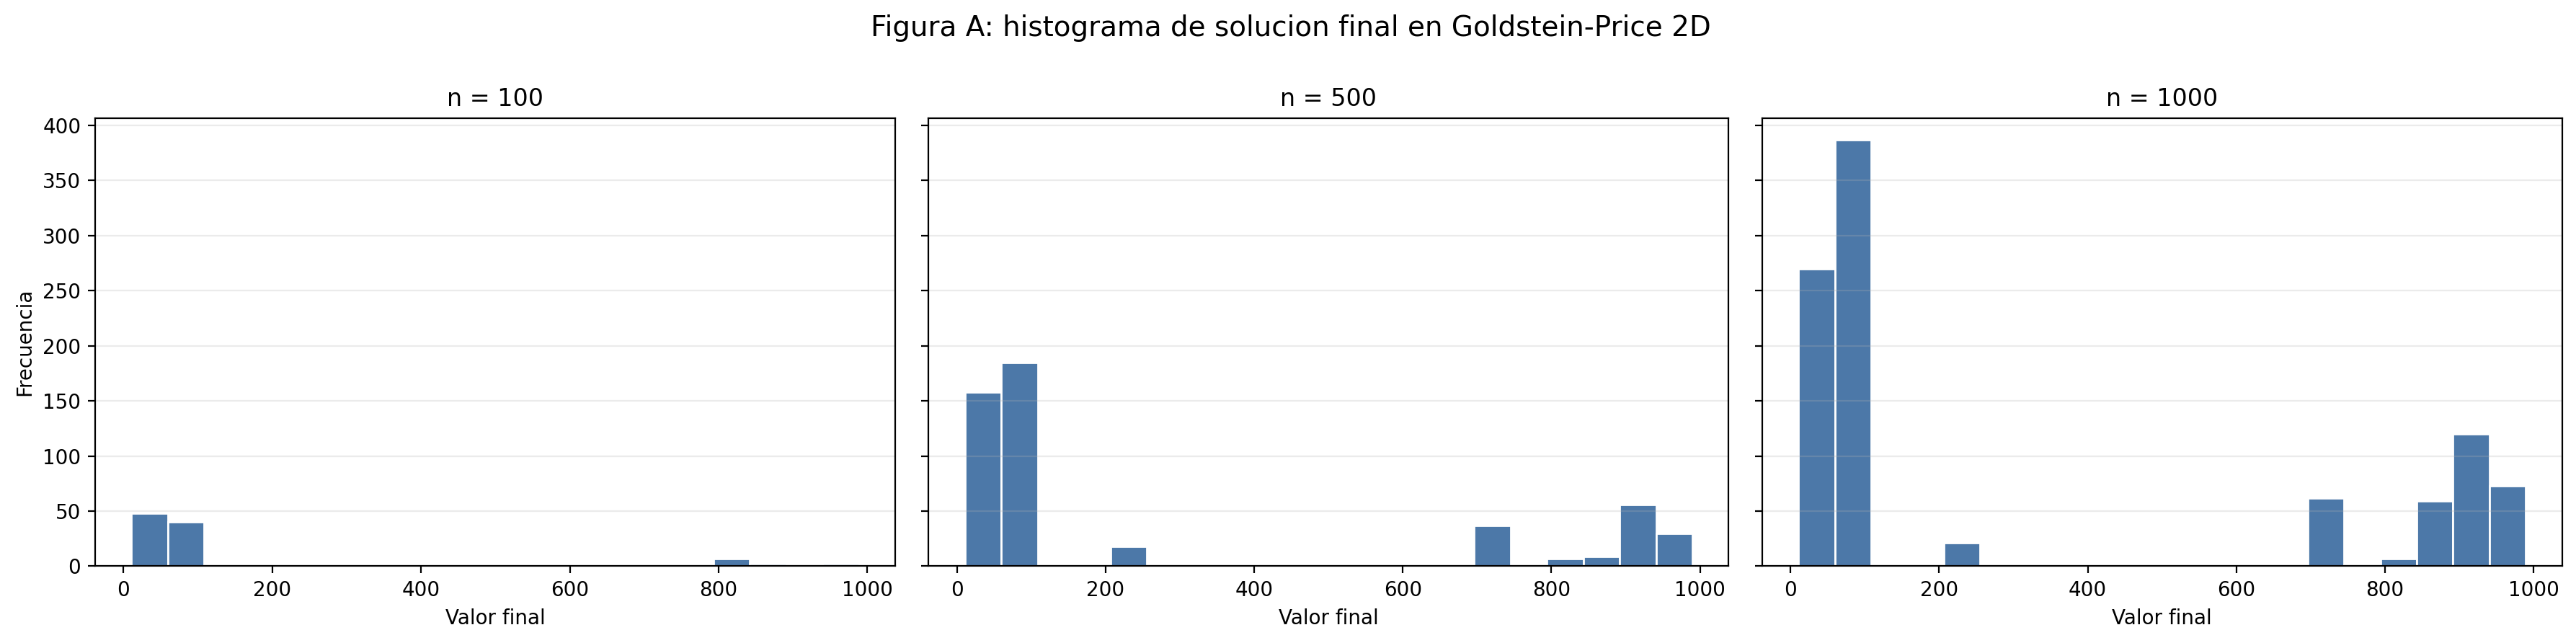
\includegraphics[keepaspectratio]{assets/numerica/gradientes/images/goldstein_price/goldstein_price_figura_a_histograma_solucion_final_2d.png}}

Se observa que en \textbf{Goldstein-Price 2D}, los histogramas muestran
una clara polarización de las frecuencias en dos extremos muy separados
(con concentraciones en los valores bajos iniciales y grandes picos que
rozan o alcanzan los 1000 en las corridas de \(n = 500\) y
\(n = 1000\)); esto evidencia una alta inestabilidad y dependencia
crítica del punto de partida, lo que demuestra que el descenso por
gradiente solo acierta y converge con éxito si cae exactamente dentro de
la cuenca de atracción correcta, terminando en mínimos locales
deficientes o divergiendo cuando esto no ocurre.

\paragraph{Six-Hump Camel}\label{six-hump-camel-2}

\subparagraph{2D}\label{d-9}

\pandocbounded{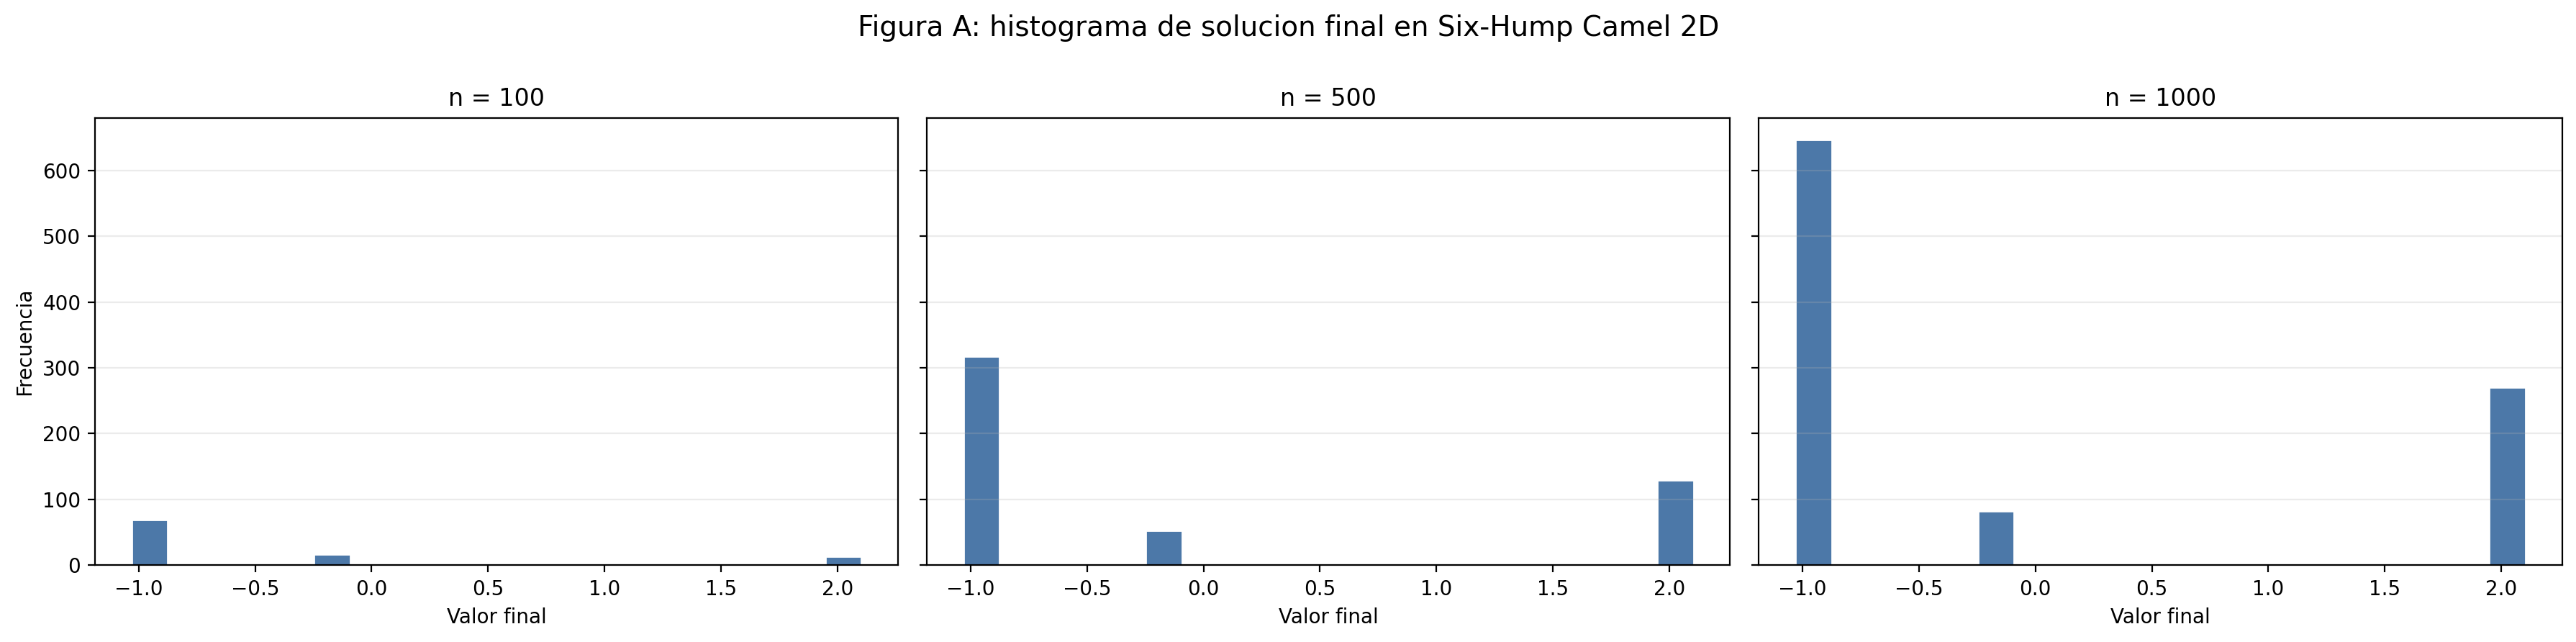
\includegraphics[keepaspectratio]{assets/numerica/gradientes/images/six_hump_camel/six_hump_camel_figura_a_histograma_solucion_final_2d.png}}

Se observa que en \textbf{Six-Hump Camel 2D}, los histogramas muestran
una fuerte concentración de las frecuencias en el valor de -1.0 (el
óptimo global) a lo largo de las distintas corridas (\(n = 100\),
\(n = 500\) y \(n = 1000\)), complementada por un grupo secundario menor
ubicado alrededor de 2.0; esto evidencia que el algoritmo es robusto y
converge de manera mayoritaria hacia la mejor solución, a pesar de que
la presencia de mínimos locales secundarios en su topología desvía
ocasionalmente algunas ejecuciones hacia el otro valor final.

\subsubsection{Histogramas de
evaluaciones}\label{histogramas-de-evaluaciones}

Además de la calidad de la solución, es fundamental medir cuántas
evaluaciones de la función objetivo fueron necesarias para alcanzar el
resultado final. Para ello se emplean histogramas del número de
evaluaciones, que permiten estudiar la eficiencia del método en cada
caso.

Estos histogramas muestran si la convergencia ocurre de manera uniforme
o si existen corridas mucho más costosas que otras. Una distribución
concentrada en valores bajos suele indicar una convergencia más
predecible y económica. En cambio, una distribución dispersa o con cola
larga sugiere que algunas ejecuciones requieren muchos más pasos para
estabilizarse, lo cual puede estar asociado a zonas complicadas del
paisaje de optimización.

La interpretación conjunta entre histogramas de valor final e
histogramas de evaluaciones es especialmente importante: un método puede
converger rápido pero hacia soluciones pobres, o puede requerir más
evaluaciones para acercarse mejor al mínimo global. Por eso, ambos
indicadores deben analizarse en conjunto y no por separado.

\paragraph{Rosenbrock}\label{rosenbrock-3}

\subparagraph{2D}\label{d-10}

\pandocbounded{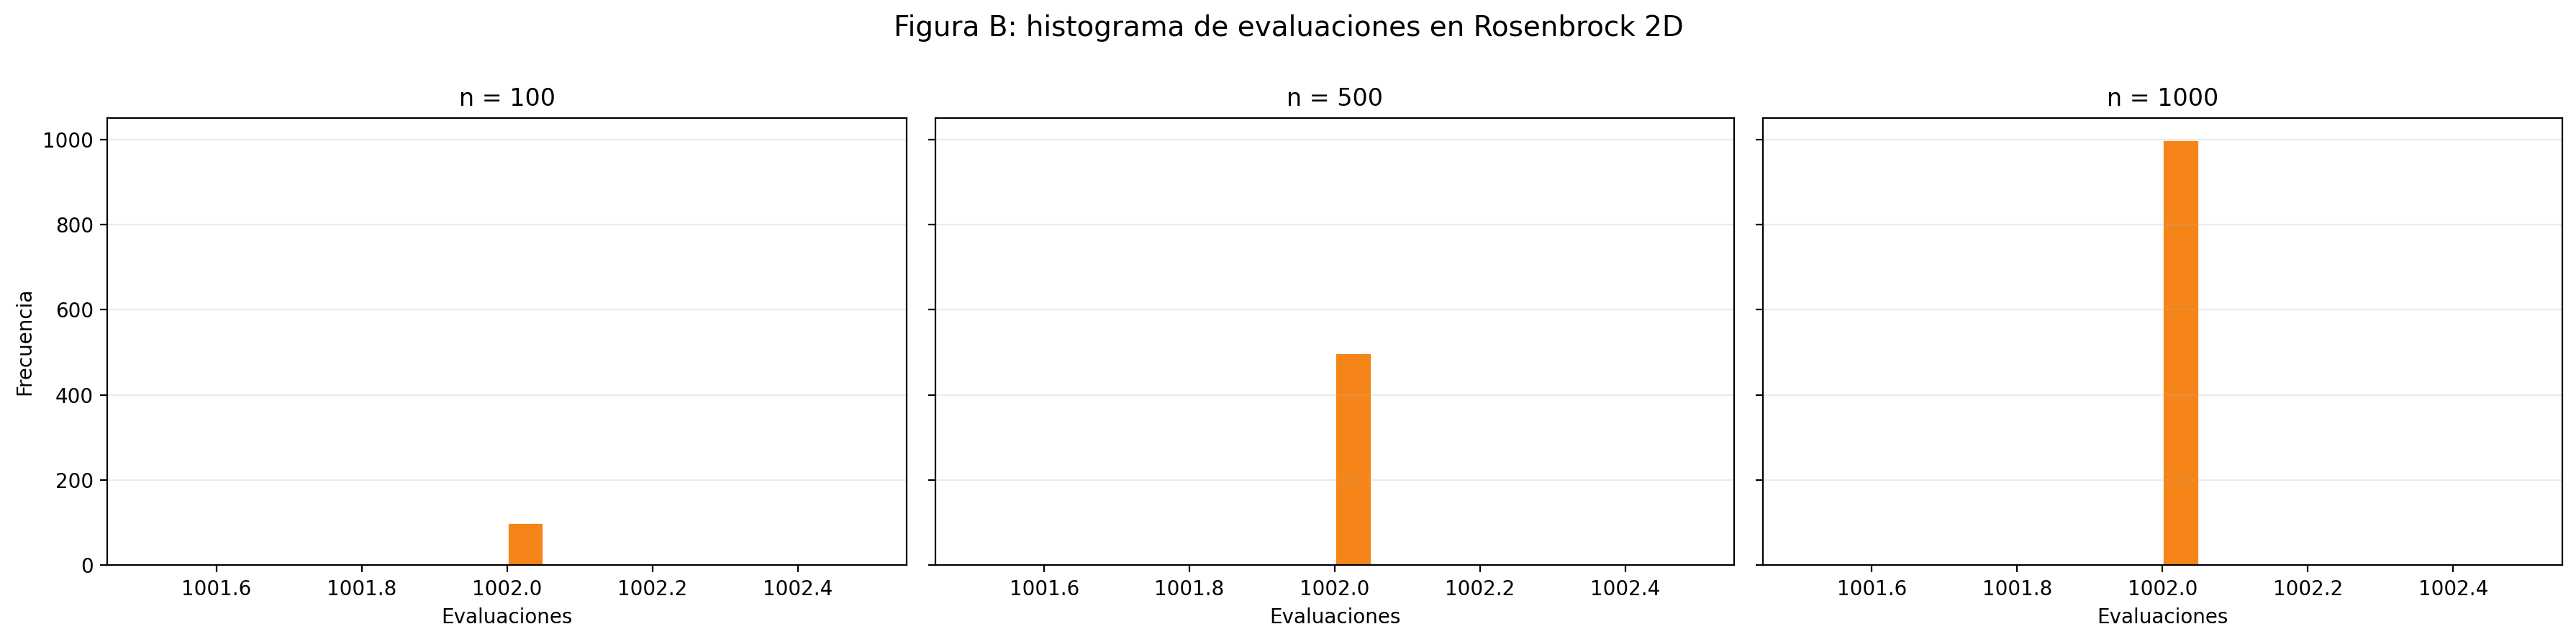
\includegraphics[keepaspectratio]{assets/numerica/gradientes/images/rosenbrock/rosenbrock_figura_b_histograma_evaluaciones_2d.png}}

\subparagraph{3D}\label{d-11}

\pandocbounded{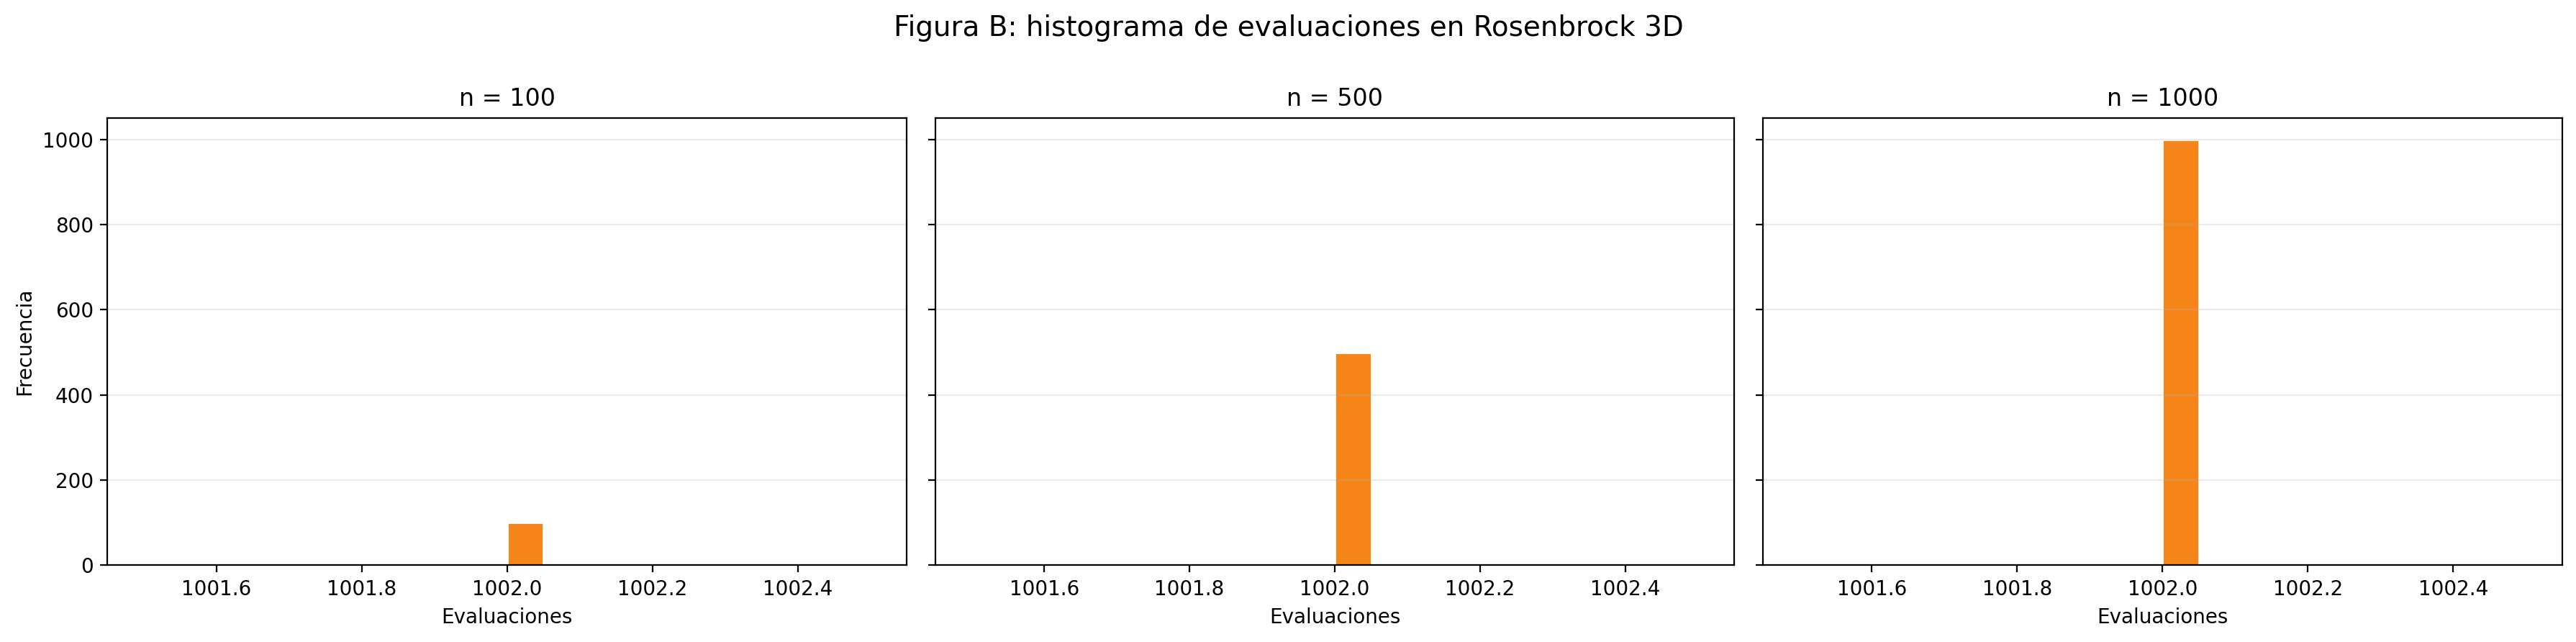
\includegraphics[keepaspectratio]{assets/numerica/gradientes/images/rosenbrock/rosenbrock_figura_b_histograma_evaluaciones_3d.png}}

Se observa que en \textbf{Rosenbrock (tanto en 2D como en 3D)}, los
histogramas muestran una frecuencia absoluta concentrada de manera
idéntica en un único valor fijo de 1002 evaluaciones; esto evidencia un
comportamiento de convergencia totalmente uniforme y predecible,
indicando que el algoritmo consume siempre exactamente el mismo esfuerzo
computacional para agotar o cumplir su criterio de parada sin importar
el tamaño de las corridas.

\paragraph{Rastrigin}\label{rastrigin-3}

\subparagraph{2D}\label{d-12}

\pandocbounded{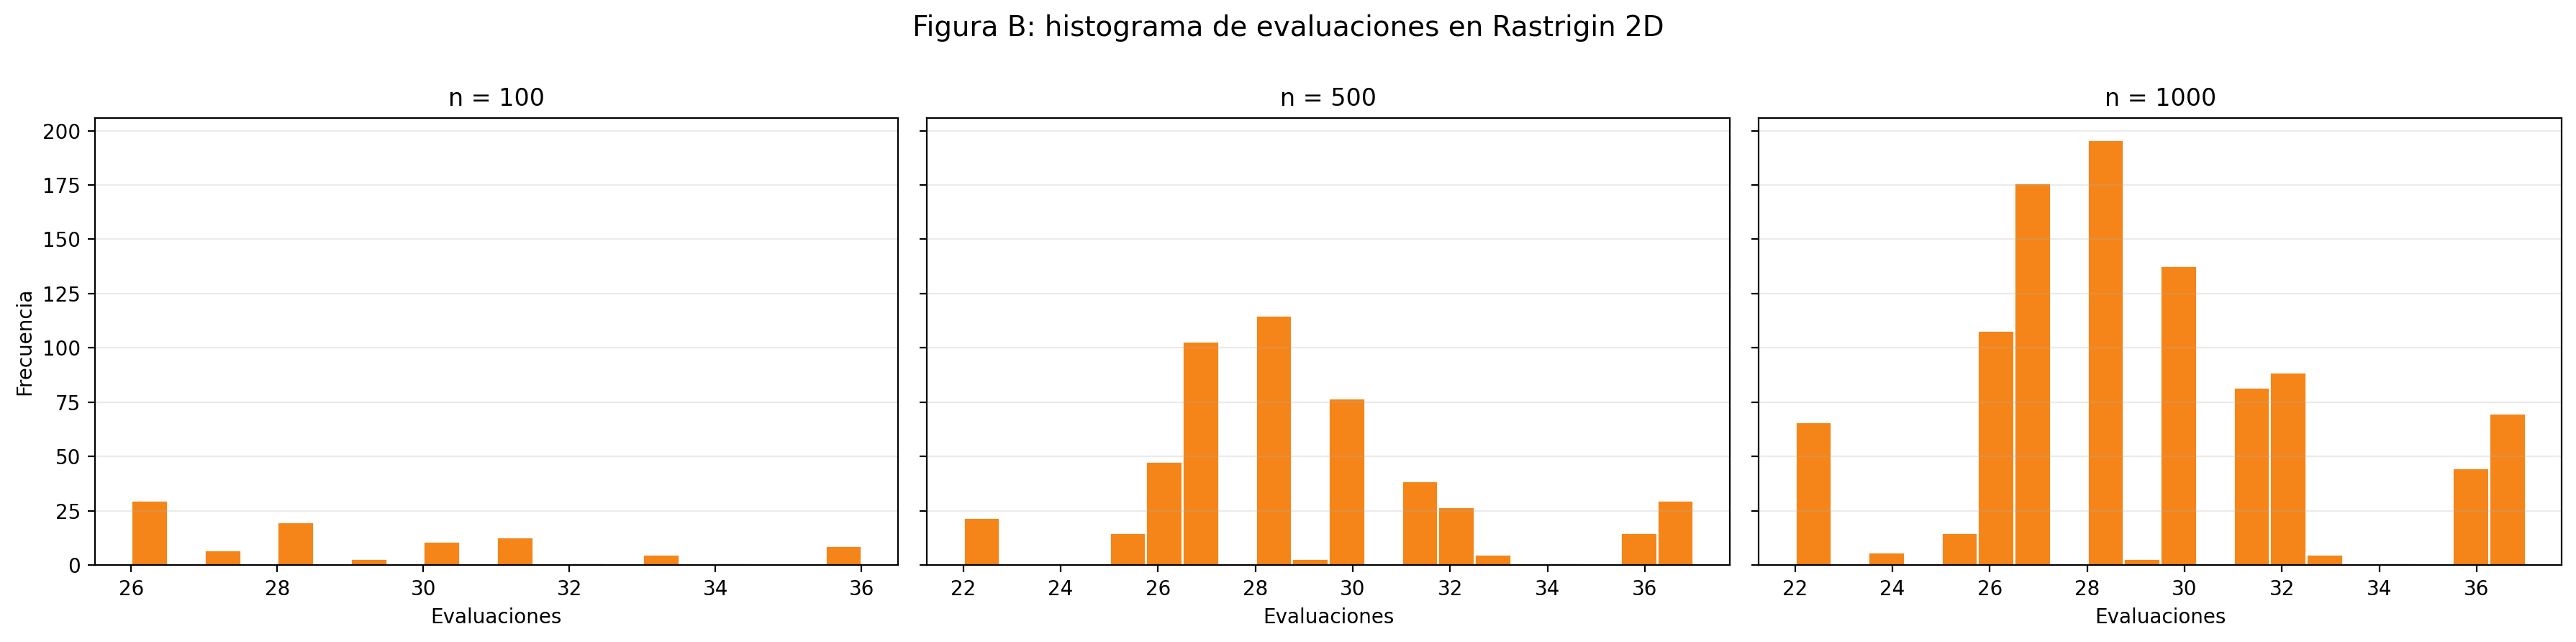
\includegraphics[keepaspectratio]{assets/numerica/gradientes/images/rastrigin/rastrigin_figura_b_histograma_evaluaciones_2d.png}}

\subparagraph{3D}\label{d-13}

\pandocbounded{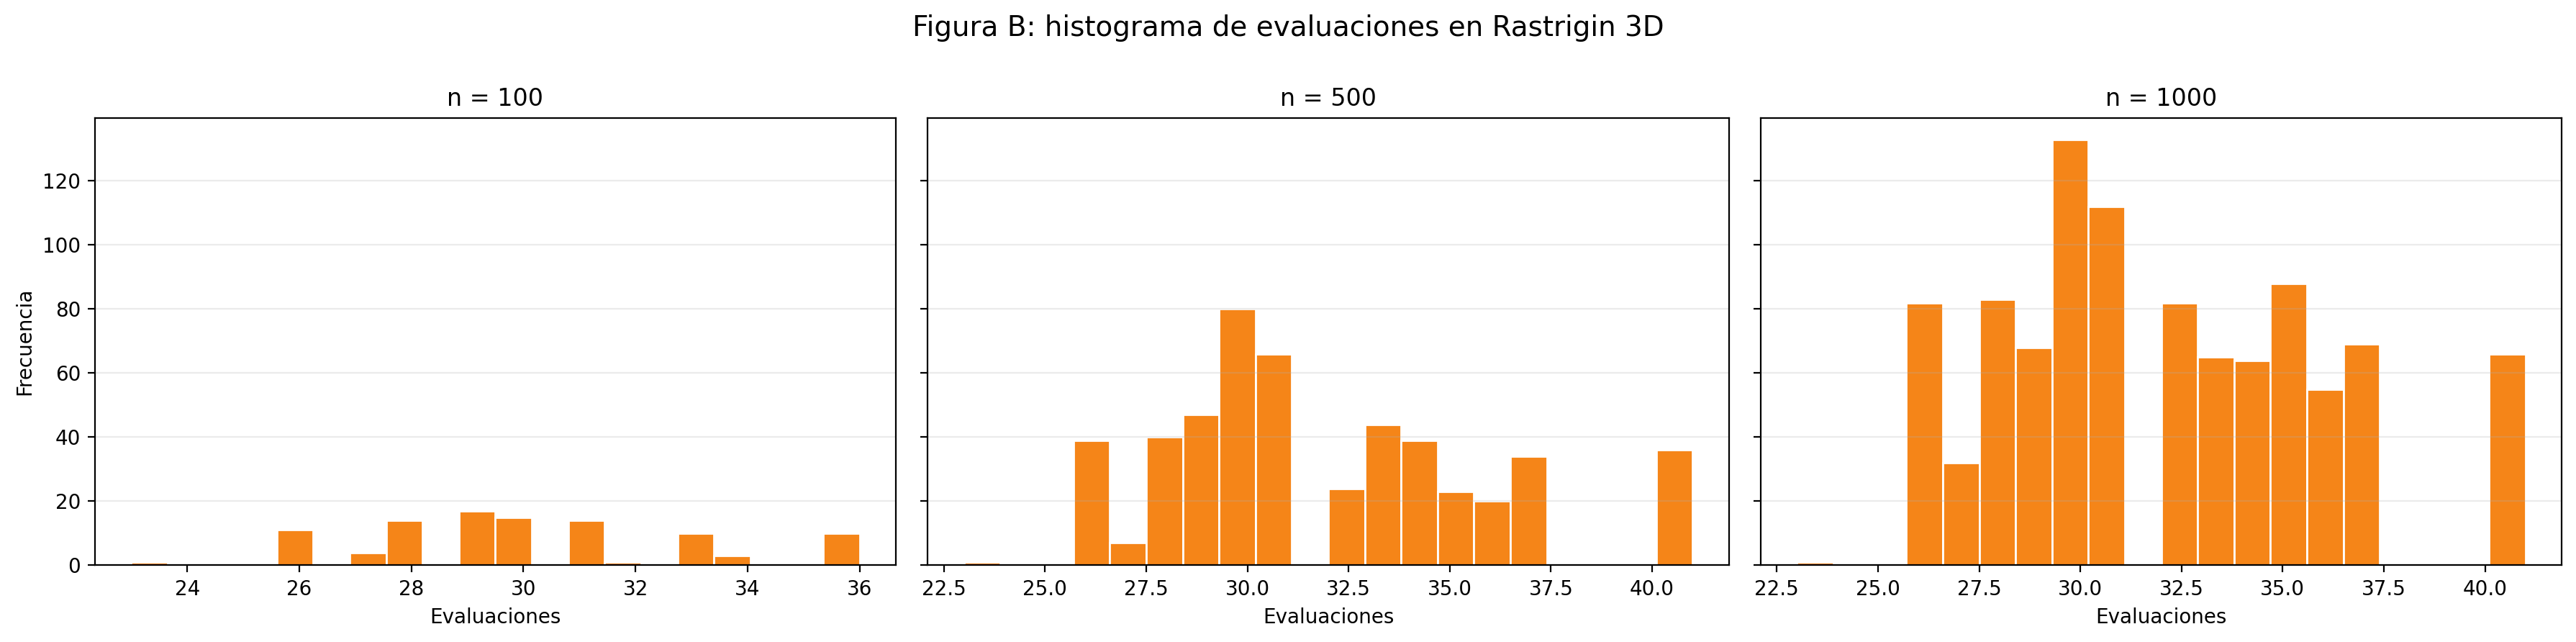
\includegraphics[keepaspectratio]{assets/numerica/gradientes/images/rastrigin/rastrigin_figura_b_histograma_evaluaciones_3d.png}}

Se observa que en \textbf{Rastrigin 2D y 3D}, los histogramas muestran
una distribución compacta y centrada de las frecuencias en un rango bajo
de evaluaciones (principalmente entre 26 y 32 pasos), lo que evidencia
que el algoritmo converge de manera muy rápida y predecible; sin
embargo, en 3D se denota una ligera extensión hacia la derecha con
frecuencias más dispersas, lo que evidencia que el aumento de
dimensionalidad incrementa ligeramente el esfuerzo computacional y la
variabilidad en algunas ejecuciones debido a los mínimos locales.

\paragraph{Schwefel}\label{schwefel-3}

\subparagraph{2D}\label{d-14}

\pandocbounded{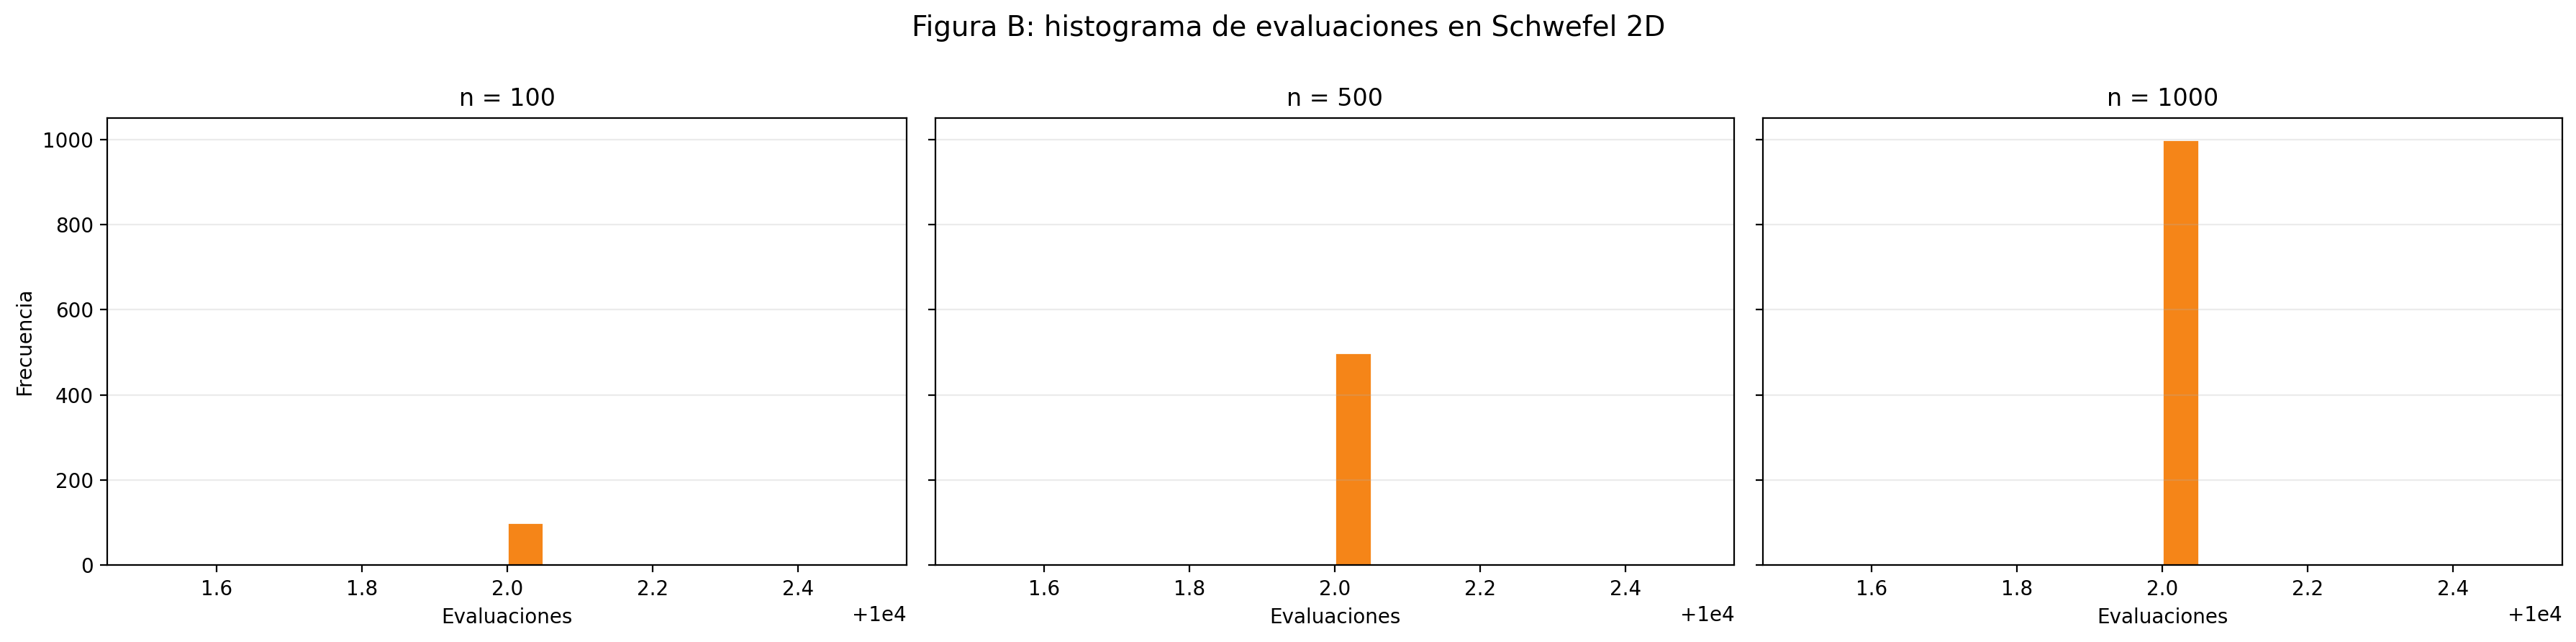
\includegraphics[keepaspectratio]{assets/numerica/gradientes/images/schwefel/schwefel_figura_b_histograma_evaluaciones_2d.png}}

\subparagraph{3D}\label{d-15}

\pandocbounded{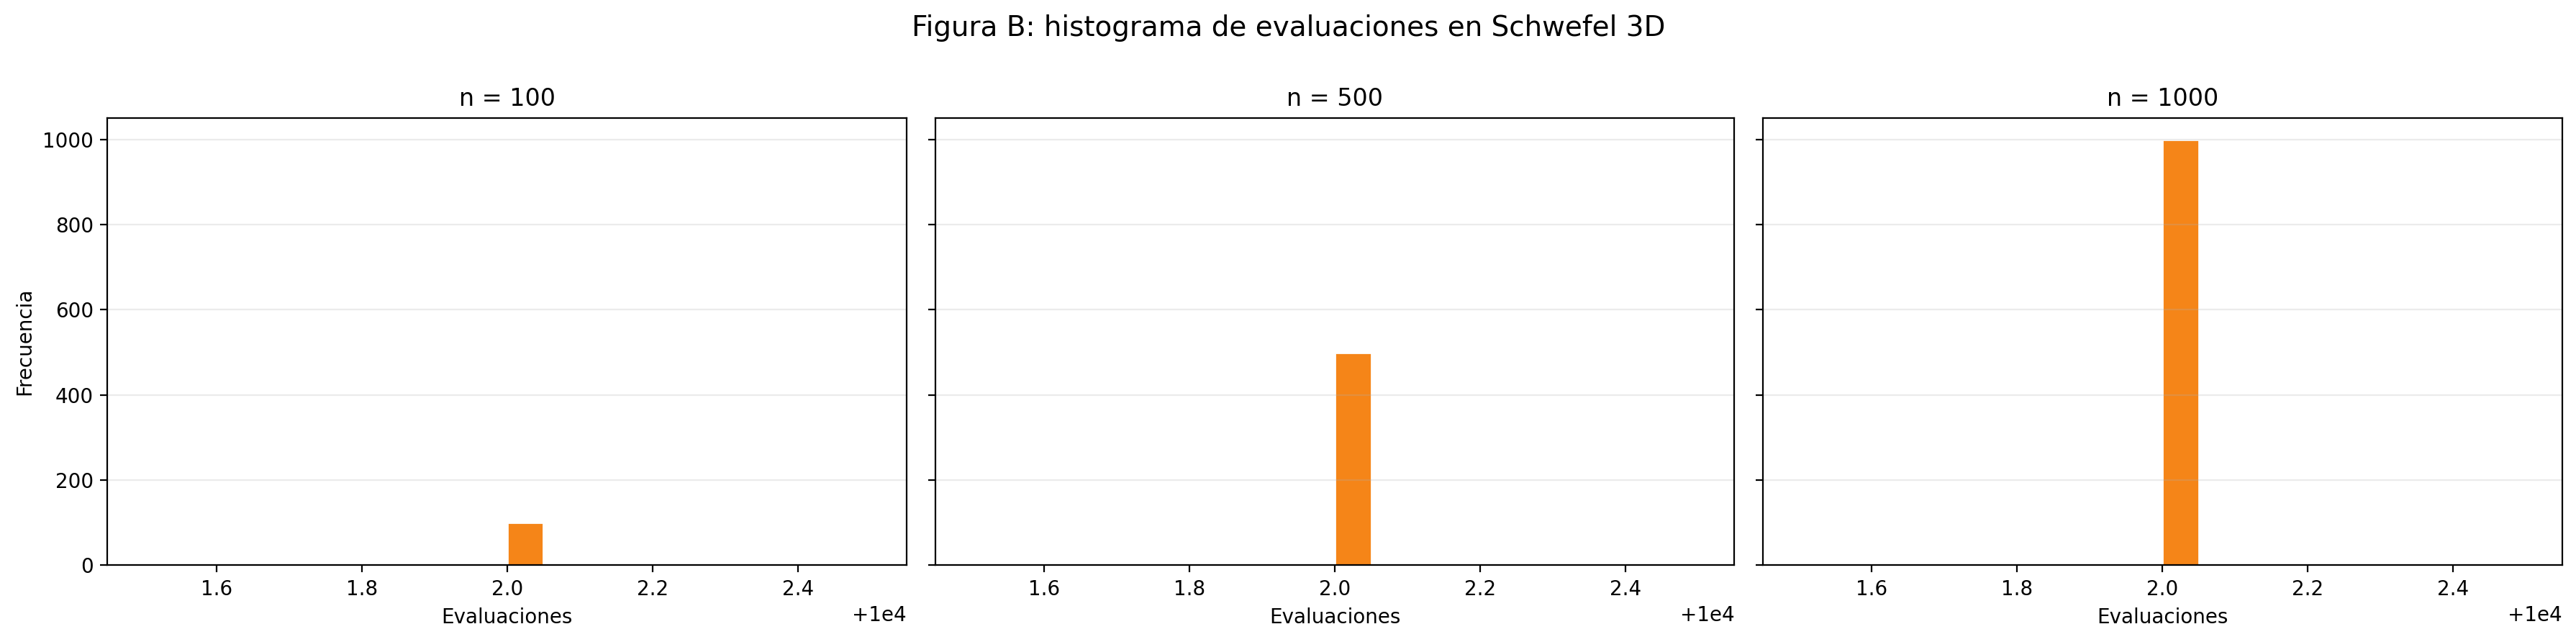
\includegraphics[keepaspectratio]{assets/numerica/gradientes/images/schwefel/schwefel_figura_b_histograma_evaluaciones_3d.png}}

Se observa que en \textbf{Schwefel (tanto en 2D como en 3D)}, los
histogramas muestran una frecuencia absoluta concentrada de manera
idéntica en un único valor fijo de aproximadamente 20000 evaluaciones
(el tope máximo configurado); esto evidencia un comportamiento de
convergencia totalmente uniforme donde el algoritmo agota por completo
sus iteraciones en todas las corridas, reflejando que no logra un
criterio de parada temprano debido a la complejidad de su búsqueda.

\paragraph{Griewank}\label{griewank-3}

\subparagraph{2D}\label{d-16}

\pandocbounded{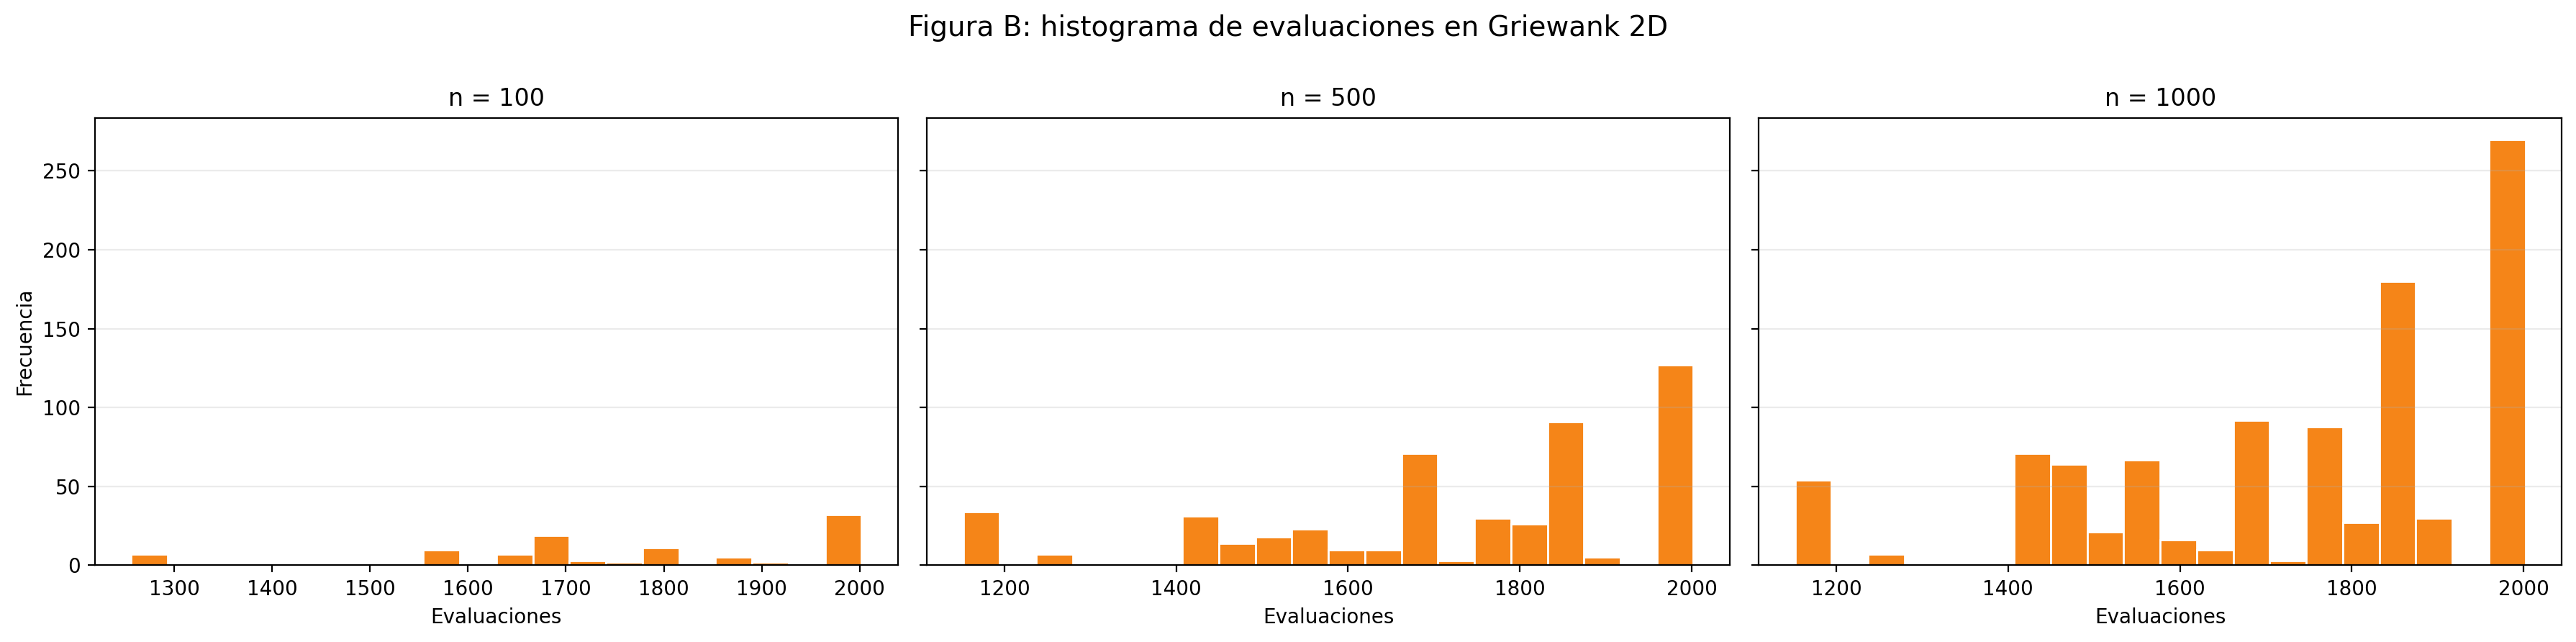
\includegraphics[keepaspectratio]{assets/numerica/gradientes/images/griewank/griewank_figura_b_histograma_evaluaciones_2d.png}}

\subparagraph{3D}\label{d-17}

\pandocbounded{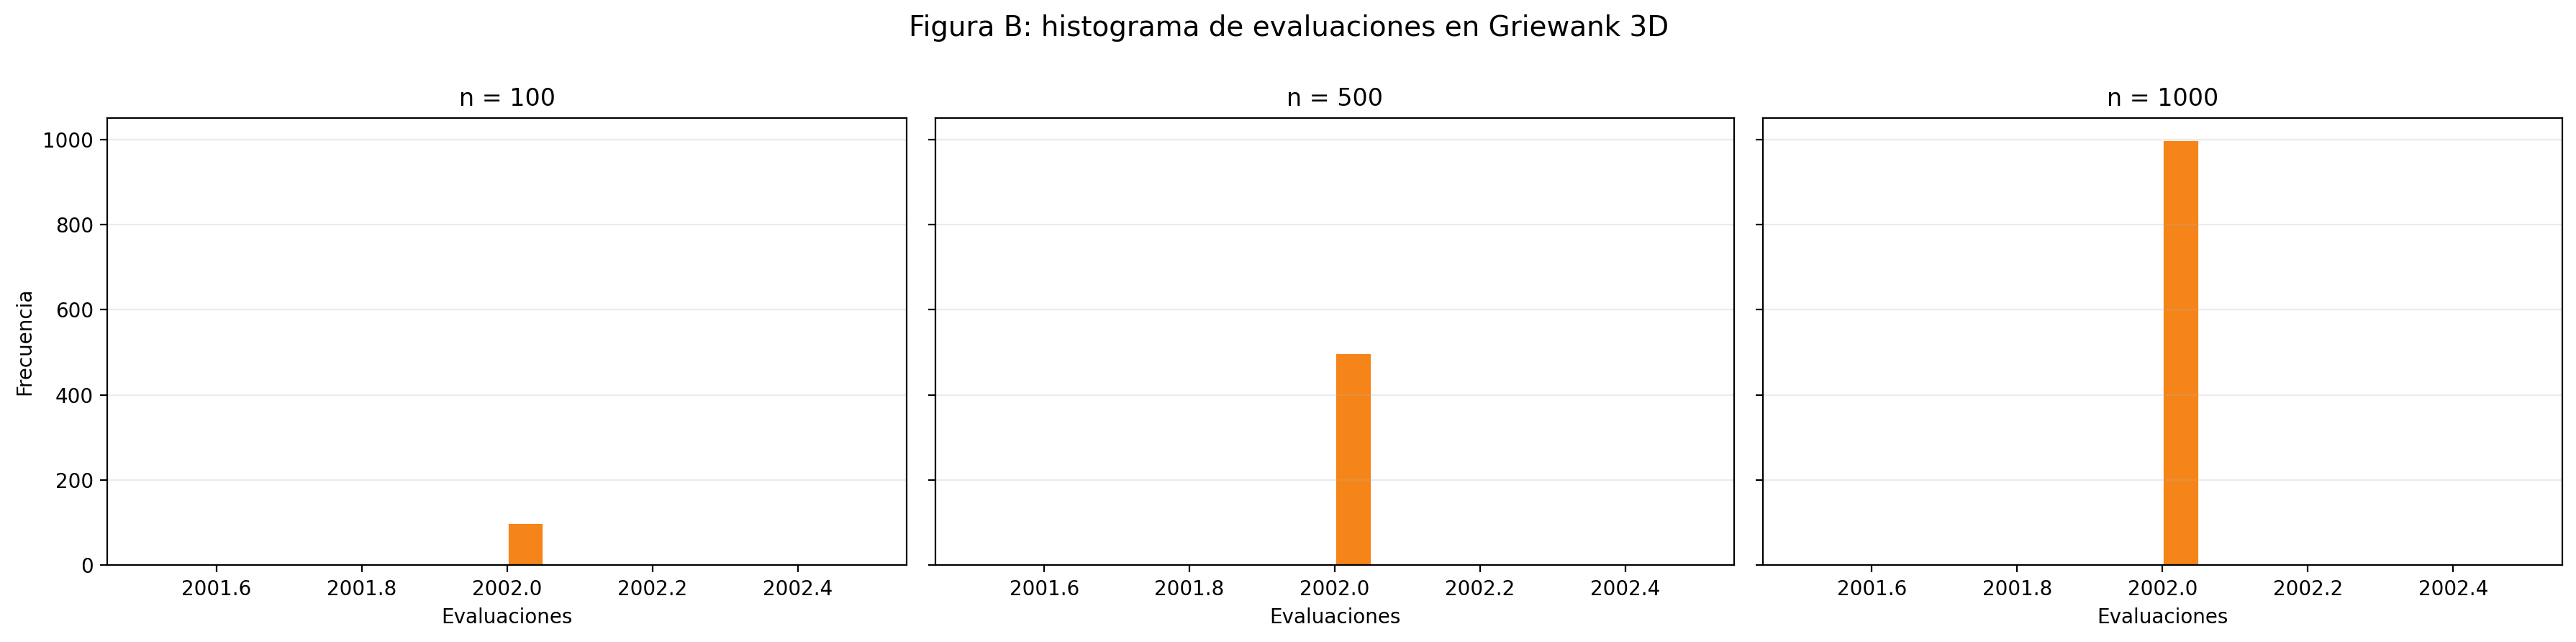
\includegraphics[keepaspectratio]{assets/numerica/gradientes/images/griewank/griewank_figura_b_histograma_evaluaciones_3d.png}}

Se observa que en \textbf{Griewank 2D}, los histogramas muestran una
distribución dispersa de las frecuencias a lo largo de un rango amplio
de evaluaciones (con un grupo notable acumulándose cerca del límite
superior de 2000 pasos), lo que evidencia que el algoritmo experimenta
una variabilidad considerable en su esfuerzo computacional según la
inicialización. Por otro lado, en \textbf{Griewank 3D}, se denota que la
frecuencia se concentra de manera absoluta en un único valor fijo de
aproximadamente 2002 evaluaciones en todas las corridas; esto evidencia
que al incrementar la dimensión, el algoritmo consume siempre el tope
máximo de pasos establecidos para cumplir su convergencia, volviéndose
completamente uniforme en su costo computacional.

\paragraph{Goldstein-Price}\label{goldstein-price-3}

\subparagraph{2D}\label{d-18}

\pandocbounded{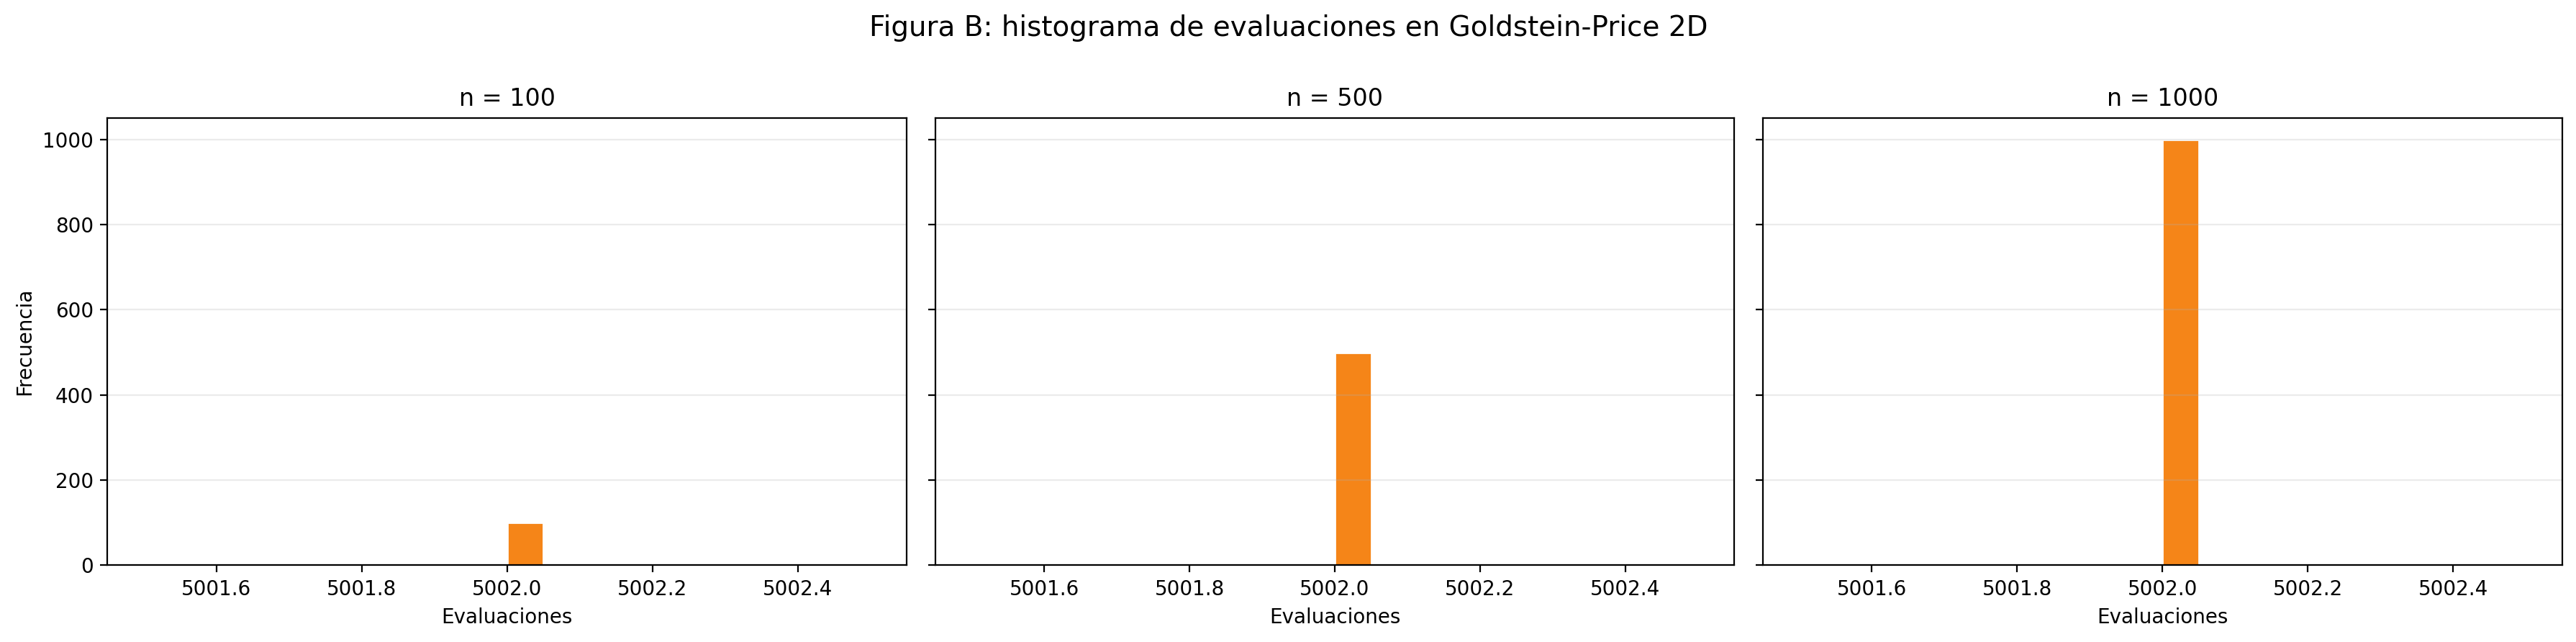
\includegraphics[keepaspectratio]{assets/numerica/gradientes/images/goldstein_price/goldstein_price_figura_b_histograma_evaluaciones_2d.png}}

Se observa que en \textbf{Goldstein-Price 2D}, los histogramas muestran
una frecuencia absoluta concentrada en un único valor fijo de 5002
evaluaciones, lo que evidencia que el algoritmo consume siempre el tope
máximo de iteraciones de manera totalmente uniforme.

\paragraph{Six-Hump Camel}\label{six-hump-camel-3}

\subparagraph{2D}\label{d-19}

\pandocbounded{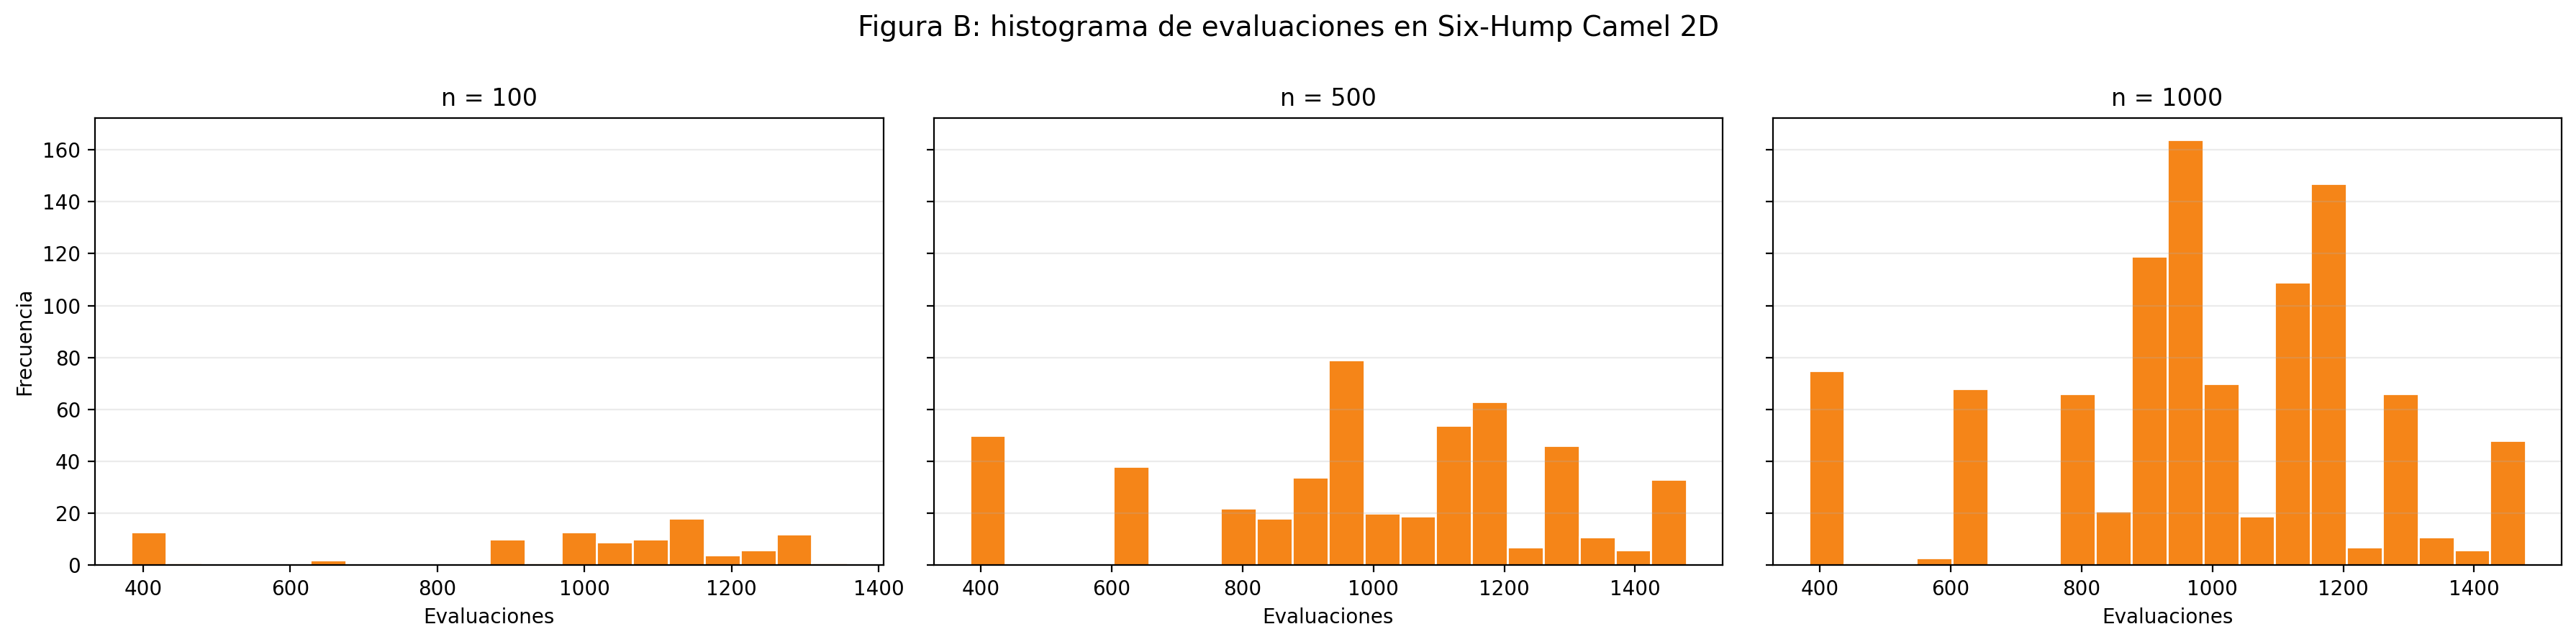
\includegraphics[keepaspectratio]{assets/numerica/gradientes/images/six_hump_camel/six_hump_camel_figura_b_histograma_evaluaciones_2d.png}}

Se observa que en \textbf{Six-Hump Camel 2D}, los histogramas muestran
una distribución dispersa y variada de las frecuencias a lo largo de un
rango amplio de evaluaciones (concentrándose principalmente entre los
800 y 1300 pasos), lo que evidencia que el algoritmo experimenta un
esfuerzo computacional heterogéneo y dependiente de la ruta de búsqueda
inicial para alcanzar la convergencia.

\subsubsection{Conclusión Parcial}\label{conclusiuxf3n-parcial}

En síntesis, el descenso por gradiente demostró ser un método eficiente
y de bajo costo en términos de evaluaciones cuando se enfrenta a
paisajes regulares (como Rosenbrock o zonas específicas de Griewank).
Sin embargo, evidenció limitaciones severas en funciones altamente
multimodales (Rastrigin y Schwefel) y superficies con valles complejos o
dependencia crítica de la inicialización (Goldstein-Price), donde el
algoritmo tiende a estancarse en mínimos locales deficientes o a
consumir el tope máximo de iteraciones sin garantizar el óptimo global.

Estas limitaciones, derivadas de su naturaleza determinista y
estrictamente local, justifican la transición hacia métodos heurísticos
de búsqueda poblacional y estocástica, los cuales favorecen un mejor
balance entre exploración y explotación del espacio de búsqueda y
resultan especialmente útiles en problemas multimodales o con paisajes
de optimización complejos (Talbi 2009).

\subsection{Optimización con Métodos
Heurísticos}\label{optimizaciuxf3n-con-muxe9todos-heuruxedsticos}

Una vez analizado el descenso por gradiente, el siguiente paso consiste
en estudiar métodos de optimización heurística que no dependan de
información derivativa de la función objetivo. En esta parte se
emplearon tres estrategias de búsqueda poblacional: \textbf{algoritmo
evolutivo}, \textbf{optimización por enjambre de partículas (PSO)} y
\textbf{evolución diferencial}. Estos métodos resultan especialmente
útiles en funciones multimodales o con paisajes complejos, donde una
estrategia puramente local puede quedar atrapada en mínimos no globales.

El objetivo de esta subsección es comparar la calidad de las soluciones
obtenidas por estos métodos, así como su costo computacional medido en
número de evaluaciones de la función objetivo. De esta manera, la
discusión no se centra solo en quién alcanza el mejor valor final, sino
también en qué tan robusto y eficiente resulta cada enfoque frente a
funciones de distinta dificultad y dimensionalidad.

\subsubsection{Metodología}\label{metodologuxeda-1}

Para el experimento heurístico se evaluaron las funciones
\texttt{Rosenbrock}, \texttt{Rastrigin}, \texttt{Schwefel} y
\texttt{Griewank} en \texttt{2D} y \texttt{3D}. Adicionalmente,
\texttt{Goldstein-Price} y \texttt{Six-Hump\ Camel} se trabajaron solo
en \texttt{2D}, ya que en el proyecto fueron implementadas en su
formulación clásica bidimensional. En todos los casos se realizaron
varias corridas con semillas distintas, registrando el mejor valor
encontrado, la mejor solución, el número de iteraciones y el número de
evaluaciones de la función objetivo.

Los resultados consolidados de esta parte fueron generados desde el
bloque \texttt{heuristicos/}, utilizando una implementación unificada
para los tres métodos y un criterio consistente de conteo de
evaluaciones. Esto permite realizar comparaciones directas entre
algoritmos bajo condiciones experimentales equivalentes.

\subsubsection{Parámetros de los
algoritmos}\label{paruxe1metros-de-los-algoritmos}

La configuración general utilizada para los experimentos heurísticos se
resume a continuación, separando los parámetros de cada método para
facilitar su lectura e interpretación.

\paragraph{Algoritmo evolutivo}\label{algoritmo-evolutivo}

{\def\LTcaptype{none} % do not increment counter
\begin{longtable}[]{@{}lr@{}}
\toprule\noalign{}
Parámetro & Valor \\
\midrule\noalign{}
\endhead
\bottomrule\noalign{}
\endlastfoot
Tamaño de población & 40 \\
Fracción de elitismo & 0.2 \\
Fracción de mutación & 0.1 \\
Máximo de iteraciones & 100 \\
\end{longtable}
}

\paragraph{PSO}\label{pso}

{\def\LTcaptype{none} % do not increment counter
\begin{longtable}[]{@{}lr@{}}
\toprule\noalign{}
Parámetro & Valor \\
\midrule\noalign{}
\endhead
\bottomrule\noalign{}
\endlastfoot
Número de partículas & 40 \\
Peso de inercia & 0.7 \\
Peso cognitivo & 1.5 \\
Peso social & 1.5 \\
Máximo de iteraciones & 100 \\
\end{longtable}
}

\paragraph{Evolución diferencial}\label{evoluciuxf3n-diferencial}

{\def\LTcaptype{none} % do not increment counter
\begin{longtable}[]{@{}lr@{}}
\toprule\noalign{}
Parámetro & Valor \\
\midrule\noalign{}
\endhead
\bottomrule\noalign{}
\endlastfoot
Tamaño de población & 40 \\
Factor de mutación & 0.8 \\
Tasa de cruce & 0.7 \\
Máximo de iteraciones & 100 \\
\end{longtable}
}

\subsubsection{Tablas de resumen
comparativo}\label{tablas-de-resumen-comparativo}

La tabla principal de esta subsección debe consolidar, para cada
función, dimensión y método, el mejor valor promedio, el mejor valor
mínimo alcanzado y el promedio de evaluaciones realizadas. Esta tabla
permite comparar de manera global tanto la calidad de las soluciones
como el costo computacional.

La siguiente tabla fue construida a partir de
\texttt{trabajo\_carlos/1.\ optimizacion\_numerica/heuristicos/datos/figuras/tabla\_resumen\_heuristicos.csv}.

{\def\LTcaptype{none} % do not increment counter
\begin{longtable}[]{@{}
  >{\raggedright\arraybackslash}p{(\linewidth - 10\tabcolsep) * \real{0.1667}}
  >{\raggedright\arraybackslash}p{(\linewidth - 10\tabcolsep) * \real{0.1667}}
  >{\raggedright\arraybackslash}p{(\linewidth - 10\tabcolsep) * \real{0.1667}}
  >{\raggedright\arraybackslash}p{(\linewidth - 10\tabcolsep) * \real{0.1667}}
  >{\raggedright\arraybackslash}p{(\linewidth - 10\tabcolsep) * \real{0.1667}}
  >{\raggedright\arraybackslash}p{(\linewidth - 10\tabcolsep) * \real{0.1667}}@{}}
\toprule\noalign{}
\begin{minipage}[b]{\linewidth}\raggedright
Función
\end{minipage} & \begin{minipage}[b]{\linewidth}\raggedright
Dimensión
\end{minipage} & \begin{minipage}[b]{\linewidth}\raggedright
Mejor método
\end{minipage} & \begin{minipage}[b]{\linewidth}\raggedright
Mejor valor mínimo
\end{minipage} & \begin{minipage}[b]{\linewidth}\raggedright
Mejor valor promedio
\end{minipage} & \begin{minipage}[b]{\linewidth}\raggedright
Promedio de evaluaciones
\end{minipage} \\
\midrule\noalign{}
\endhead
\bottomrule\noalign{}
\endlastfoot
Rosenbrock & 2 & Evolución diferencial & 0.000000 & 0.000000 & 4840.0 \\
Rosenbrock & 3 & Evolución diferencial & 0.000002 & 0.000242 & 4840.0 \\
Rastrigin & 2 & Evolución diferencial & 0.000000 & 0.000000 & 4840.0 \\
Rastrigin & 3 & Evolución diferencial & 0.000002 & 0.038206 & 4840.0 \\
Schwefel & 2 & Evolución diferencial & 0.000025 & 0.000025 & 7050.0 \\
Schwefel & 3 & Evolución diferencial & 0.000038 & 0.000038 & 7050.0 \\
Griewank & 2 & PSO & 0.000000 & 0.002583 & 7050.0 \\
Griewank & 3 & PSO & 0.000000 & 0.009003 & 7050.0 \\
Goldstein-Price & 2 & Evolución diferencial & 3.000000 & 3.000000 &
4840.0 \\
Six-Hump Camel & 2 & PSO & -1.031628 & -1.031628 & 4840.0 \\
\end{longtable}
}

En general, la tabla resume un patrón bastante claro:
\texttt{Evolución\ diferencial} es el método más sólido en la mayoría de
las funciones analizadas. En \texttt{Rosenbrock}, \texttt{Rastrigin},
\texttt{Schwefel} y \texttt{Goldstein-Price}, este método alcanza los
mejores valores promedio y, al mismo tiempo, mantiene un costo
computacional estable, lo que sugiere una buena combinación entre
precisión y robustez frente a distintos paisajes de optimización.

Por su parte, \texttt{PSO} sobresale en \texttt{Griewank} y
\texttt{Six-Hump\ Camel}. En estos casos logra los mejores valores
promedio, lo que indica que su dinámica de exploración y ajuste
colectivo se adapta especialmente bien a superficies con múltiples
mínimos, pero con una estructura más favorable. Esto muestra que no
existe un único método universalmente superior, aunque sí se observa una
ventaja general de \texttt{Evolución\ diferencial} en los problemas más
exigentes.

También se nota que la dimensión influye de manera importante en la
dificultad. Al pasar de \texttt{2D} a \texttt{3D}, funciones como
\texttt{Rosenbrock}, \texttt{Rastrigin}, \texttt{Schwefel} y
\texttt{Griewank} presentan un deterioro en el valor promedio, lo que
refleja que el aumento de dimensionalidad hace más compleja la búsqueda
del óptimo global. Aun así, los métodos mejor posicionados conservan un
desempeño competitivo, lo que refuerza la utilidad de estos enfoques
heurísticos para problemas no convexos y multimodales.

En síntesis, los resultados sugieren que \texttt{Evolución\ diferencial}
es la alternativa más consistente como método general, mientras que
\texttt{PSO} puede ser preferible en funciones específicas donde la
estructura del paisaje favorece su estrategia de búsqueda.

\subsubsection{Comparación gráfica de
desempeño}\label{comparaciuxf3n-gruxe1fica-de-desempeuxf1o}

Para evitar una presentación excesivamente fragmentada, en la parte
heurística conviene resumir los resultados con unas pocas figuras
comparativas de alto valor interpretativo. En lugar de repetir una
gráfica por cada función y por cada método, es preferible usar figuras
consolidadas que permitan identificar rápidamente tendencias generales.

\subsubsection{Comparación gráfica de la mediana del valor
final}\label{comparaciuxf3n-gruxe1fica-de-la-mediana-del-valor-final}

\paragraph{Función Rosenbrock}\label{funciuxf3n-rosenbrock}

\pandocbounded{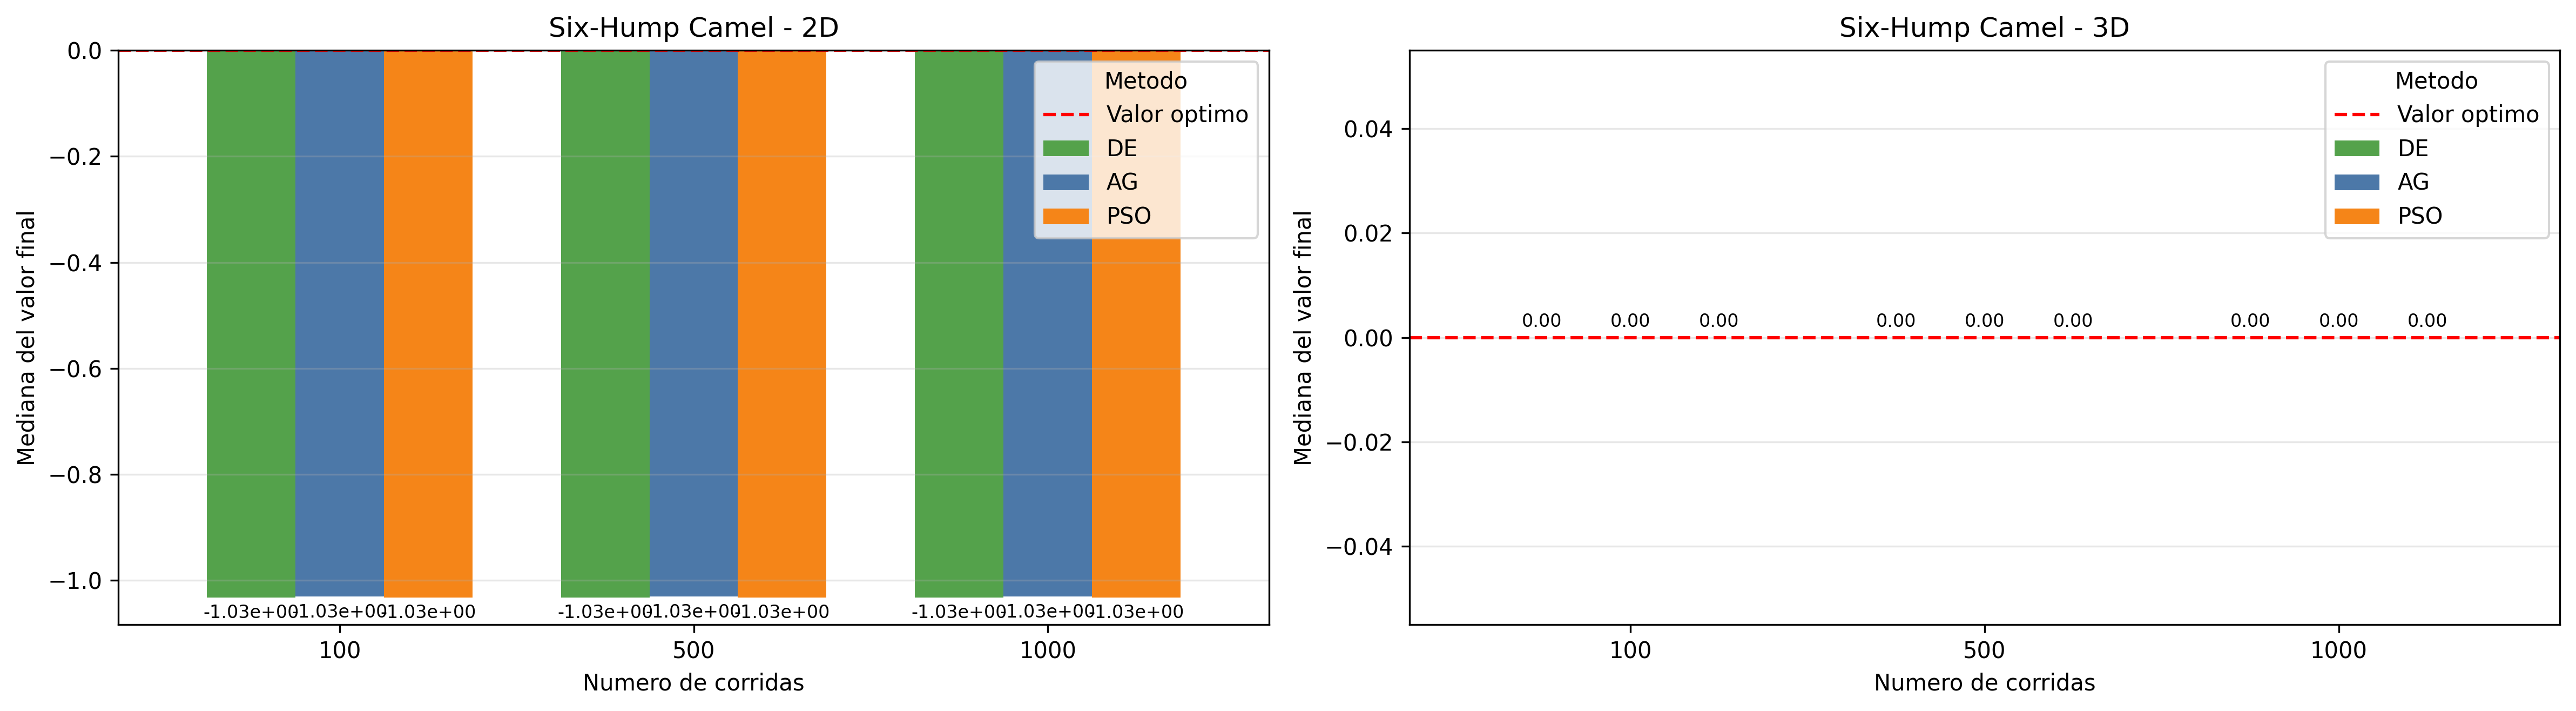
\includegraphics[keepaspectratio]{assets/numerica/heuristicos/images/rosenbrock/rosenbrock_2d_3d_corridas.png}}

En \texttt{Rosenbrock}, \texttt{Evolución\ diferencial} logra los
mejores resultados en \texttt{2D} y \texttt{3D}, con valores muy
cercanos al óptimo. Al aumentar la dimensión, \texttt{PSO} y el
\texttt{Algoritmo\ evolutivo} pierden algo de precisión.

\paragraph{Función Rastrigin}\label{funciuxf3n-rastrigin}

\pandocbounded{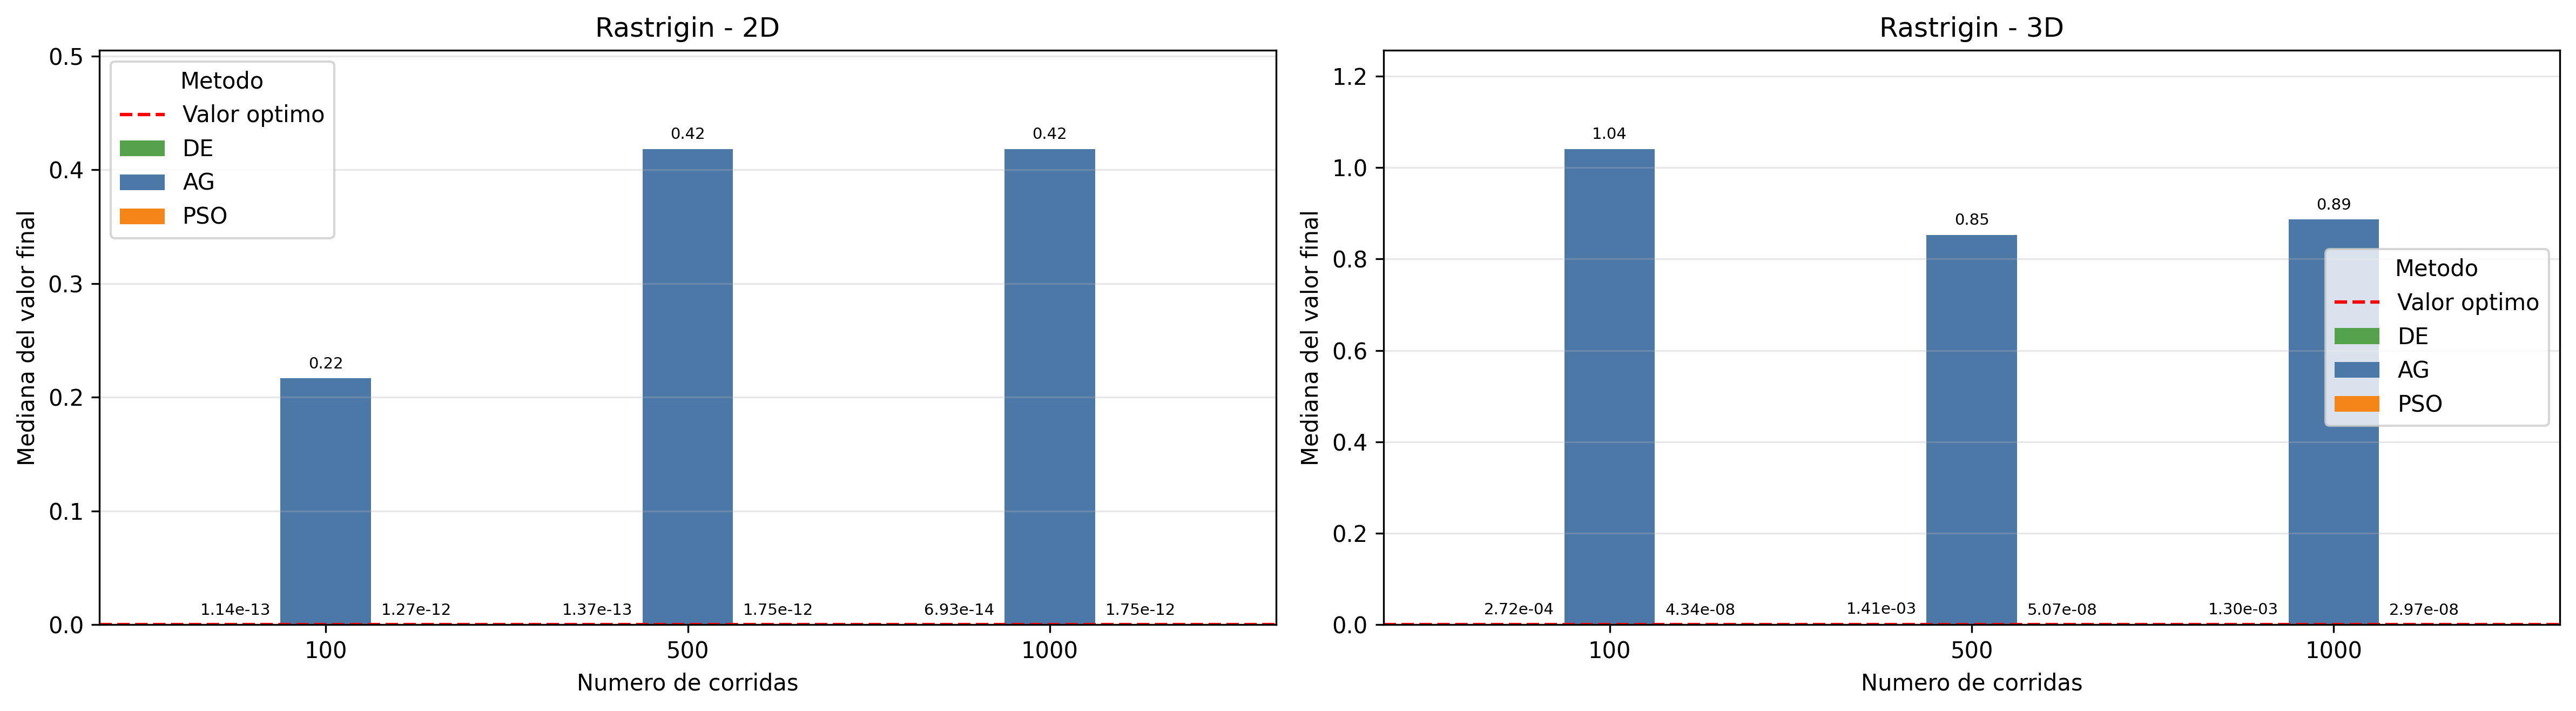
\includegraphics[keepaspectratio]{assets/numerica/heuristicos/images/rastrigin/rastrigin_2d_3d_corridas.png}}

En \texttt{Rastrigin}, \texttt{Evolución\ diferencial} y \texttt{PSO}
mantienen valores casi nulos en ambas dimensiones. El
\texttt{Algoritmo\ evolutivo} muestra mayores dificultades, sobre todo
en \texttt{3D}.

\paragraph{Función Schwefel}\label{funciuxf3n-schwefel}

\pandocbounded{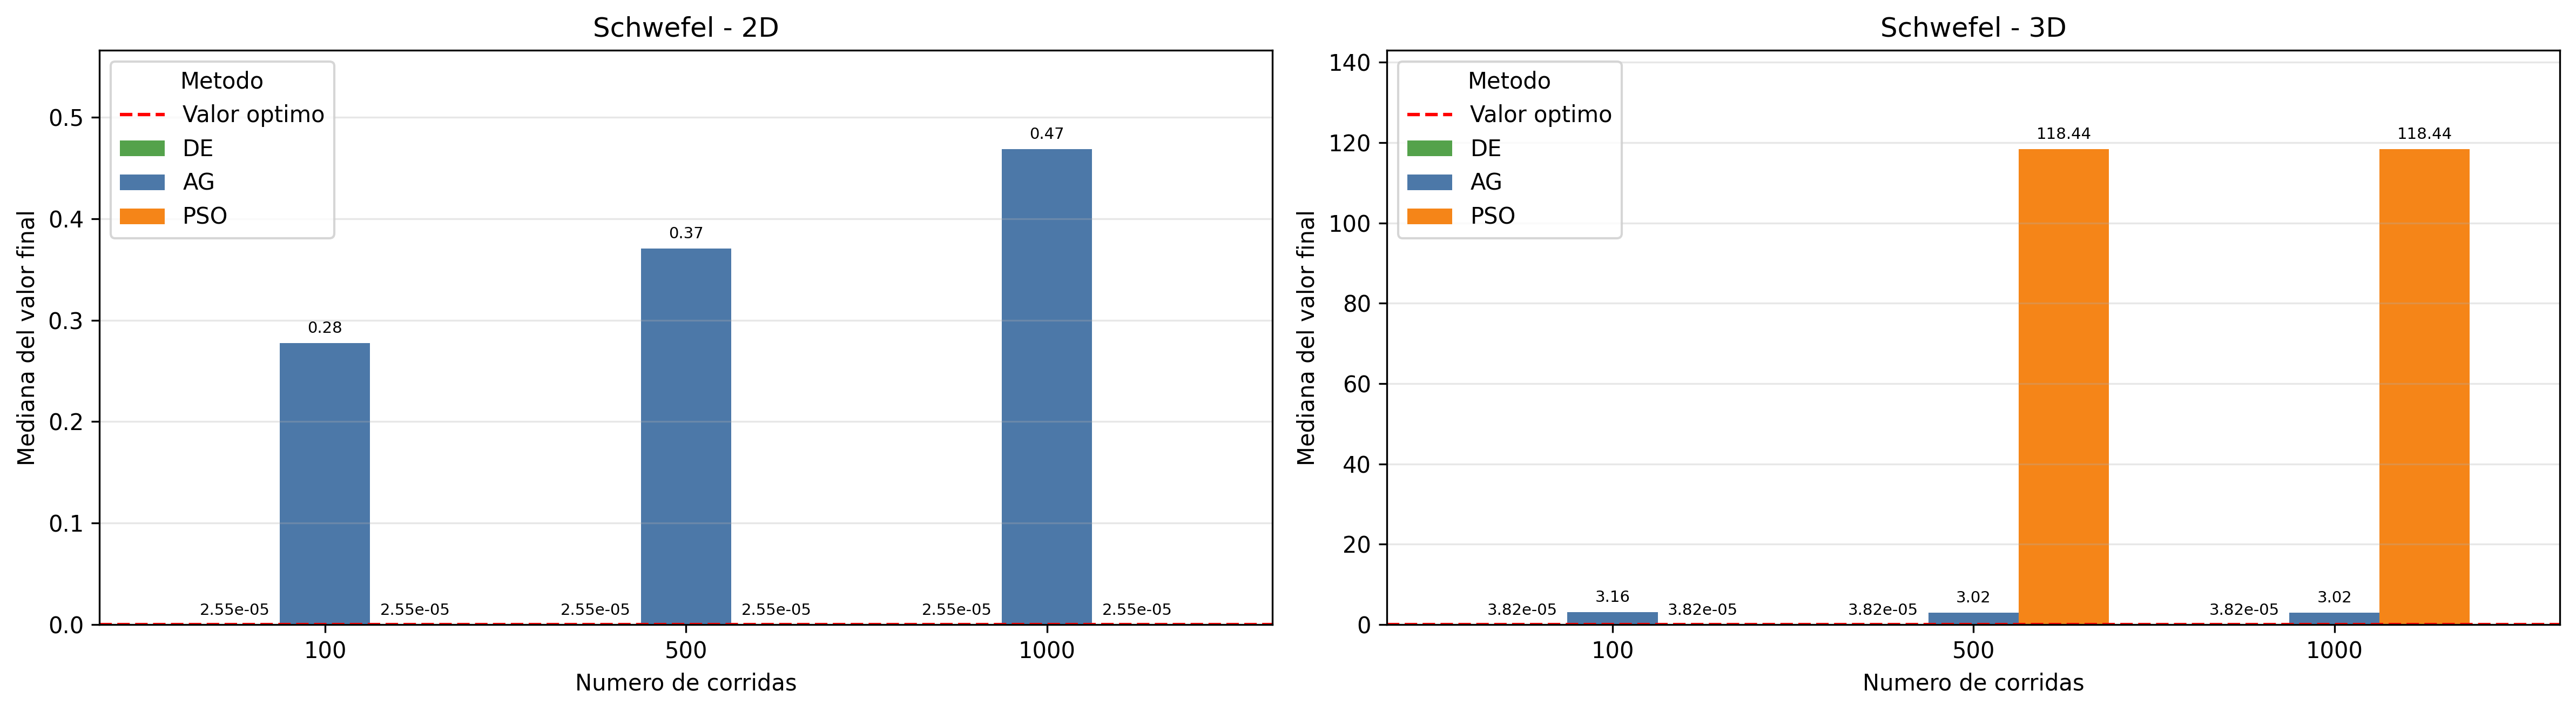
\includegraphics[keepaspectratio]{assets/numerica/heuristicos/images/schwefel/schwefel_2d_3d_corridas.png}}

En \texttt{Schwefel}, \texttt{Evolución\ diferencial} es el método más
estable y preciso en \texttt{2D} y \texttt{3D}. En cambio, \texttt{PSO}
empeora con fuerza en \texttt{3D}, mostrando la mayor sensibilidad a la
dimensión.

\paragraph{Función Griewank}\label{funciuxf3n-griewank}

\pandocbounded{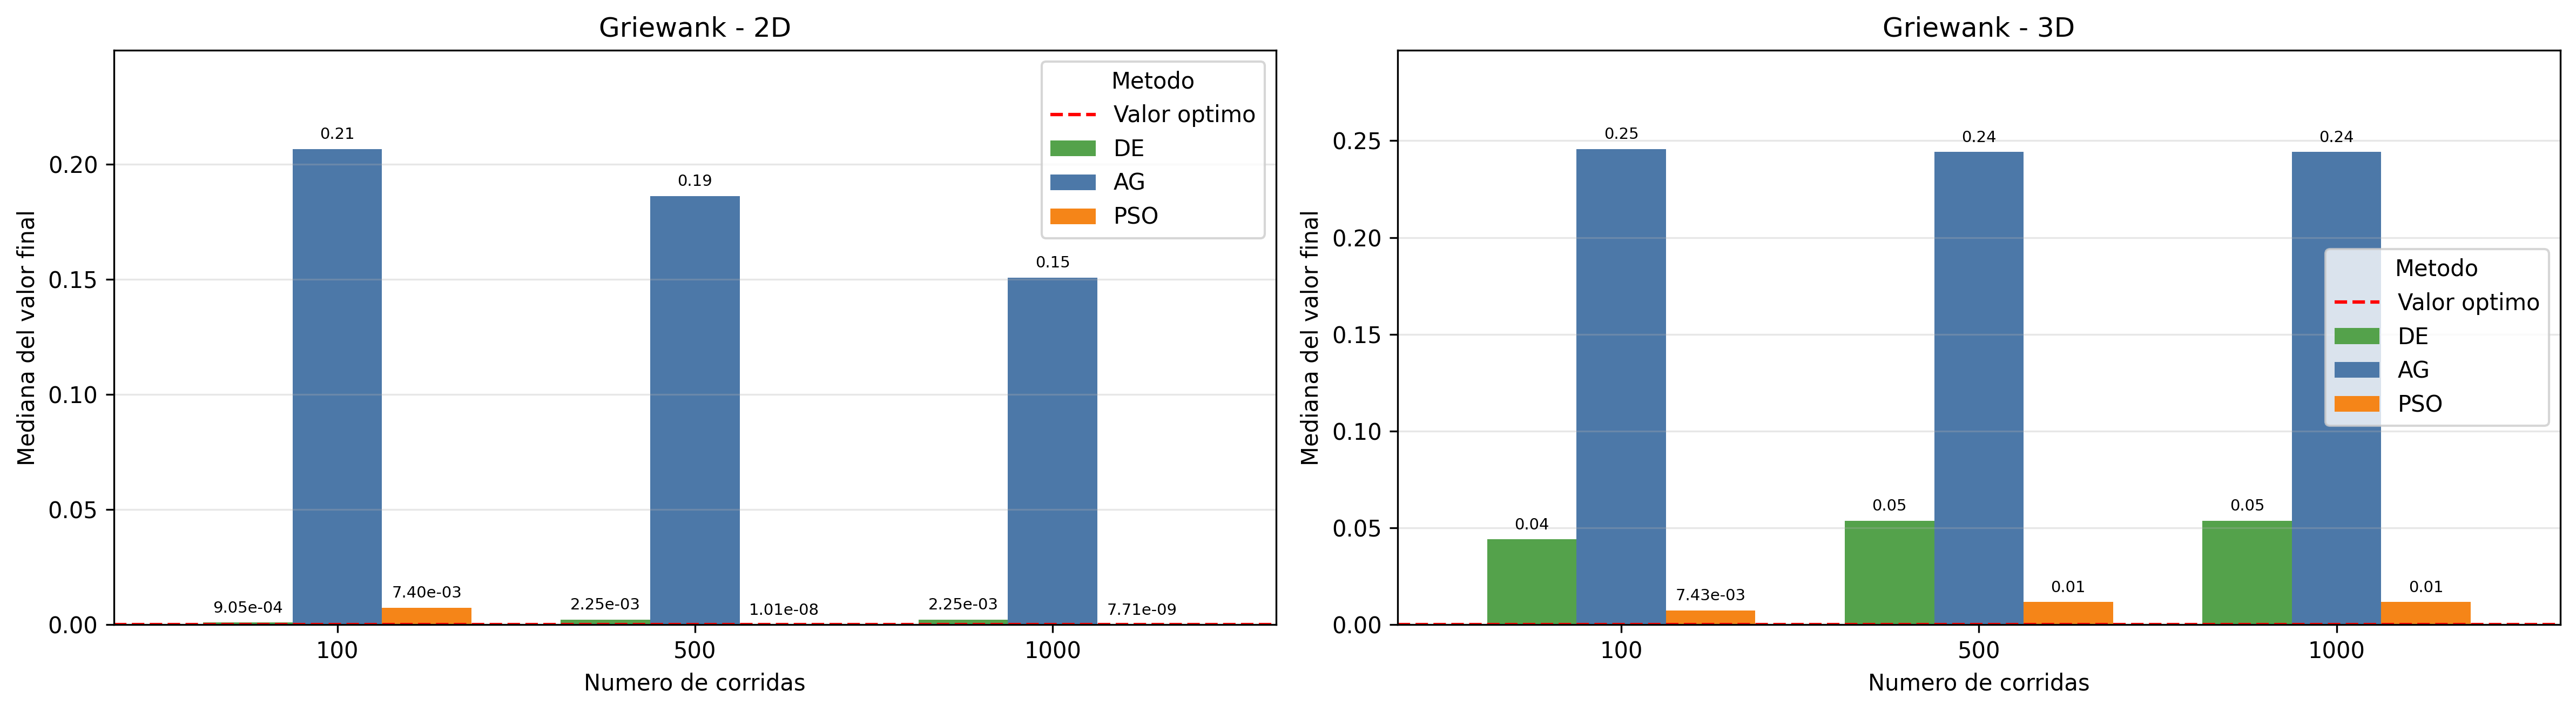
\includegraphics[keepaspectratio]{assets/numerica/heuristicos/images/griewank/griewank_2d_3d_corridas.png}}

En \texttt{Griewank}, \texttt{PSO} presenta el mejor desempeño general,
con valores más cercanos al óptimo en \texttt{2D} y \texttt{3D}.
\texttt{Evolución\ diferencial} también responde bien, mientras que el
\texttt{Algoritmo\ evolutivo} queda más rezagado.

\paragraph{Función Goldstein-Price}\label{funciuxf3n-goldstein-price}

\pandocbounded{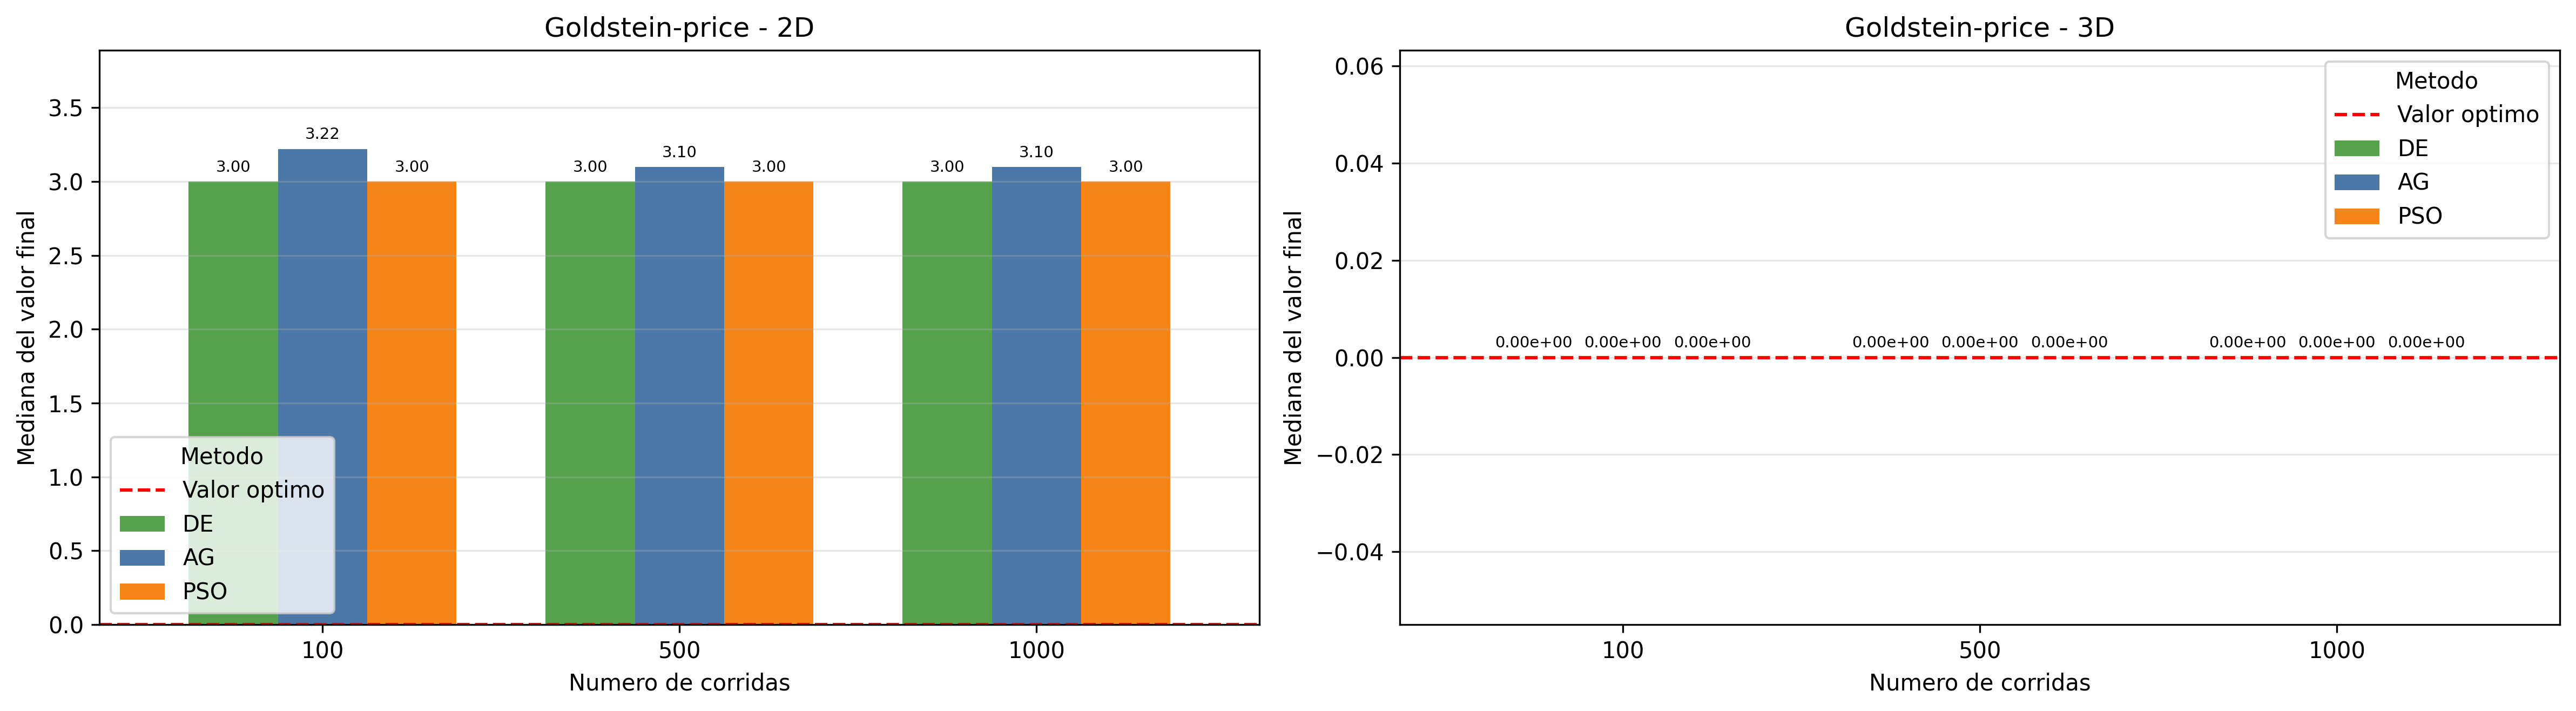
\includegraphics[keepaspectratio]{assets/numerica/heuristicos/images/goldstein-price/goldstein-price_2d_3d_corridas.png}}

En \texttt{Goldstein-Price}, los tres métodos tienen resultados
parecidos, aunque \texttt{Evolución\ diferencial} y \texttt{PSO} se
mantienen más cerca del valor óptimo. El \texttt{Algoritmo\ evolutivo}
presenta una precisión ligeramente menor.

\paragraph{Función Six-Hump Camel}\label{funciuxf3n-six-hump-camel-1}

\pandocbounded{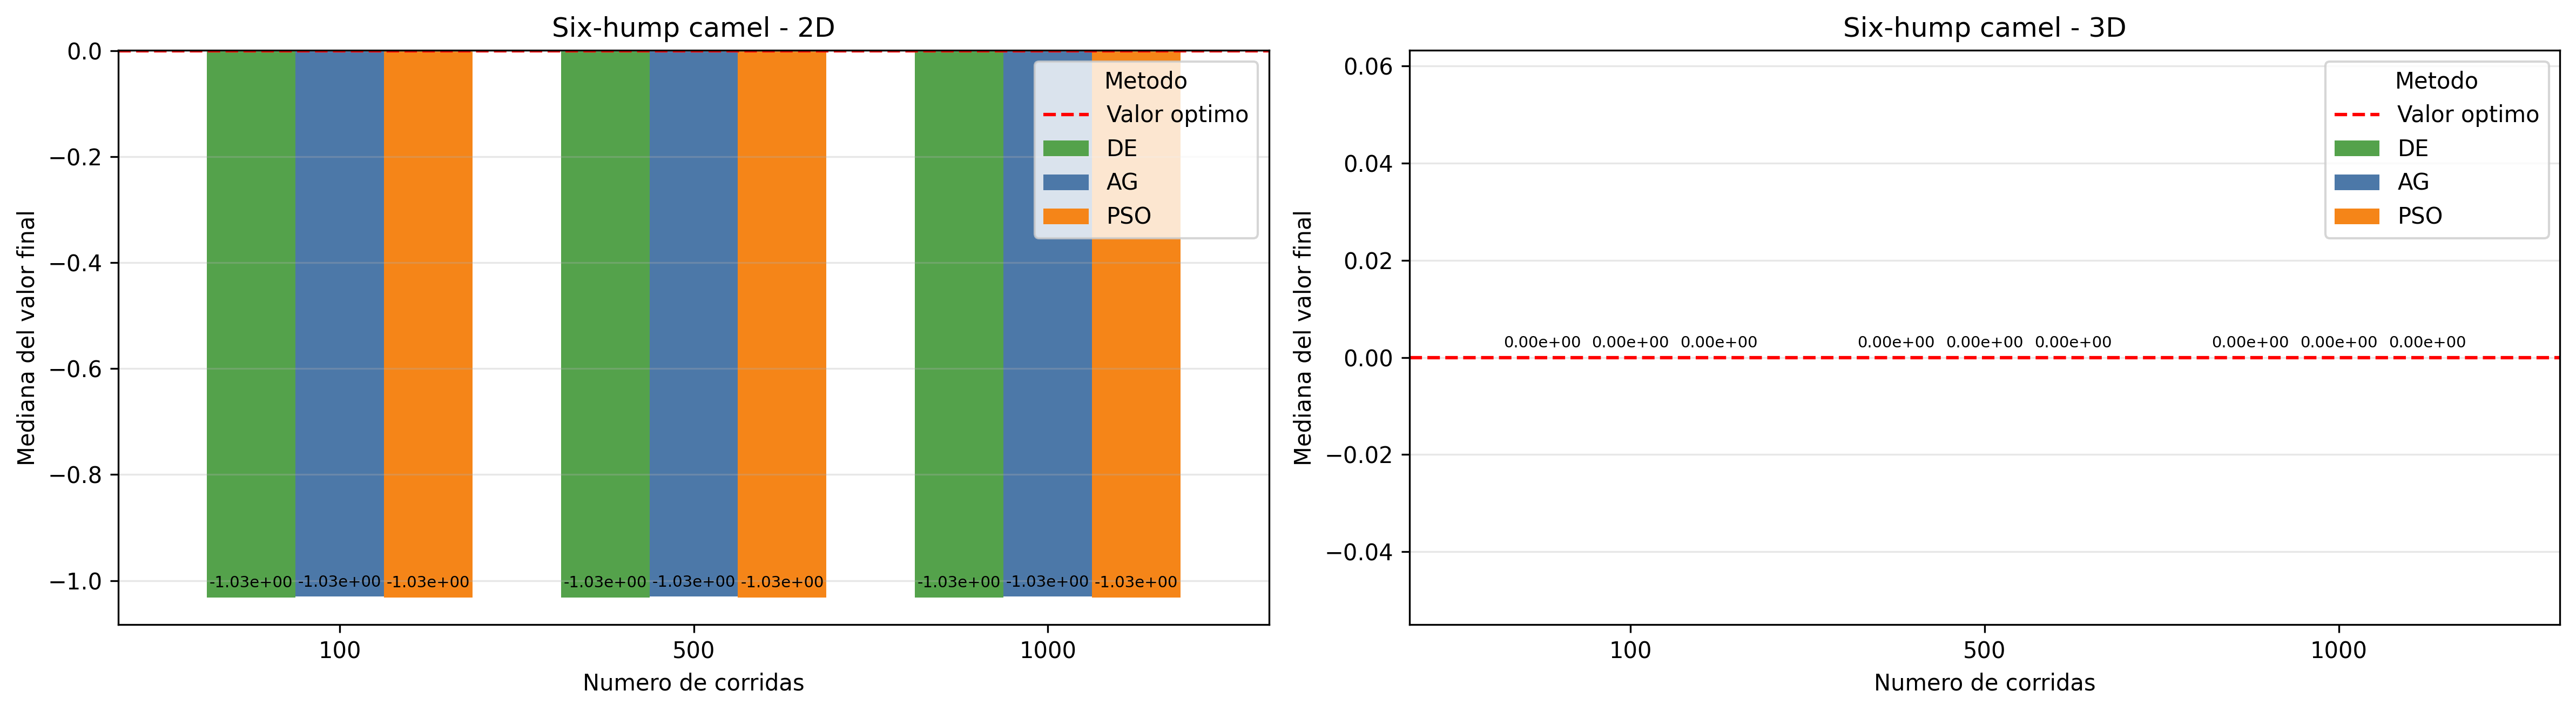
\includegraphics[keepaspectratio]{assets/numerica/heuristicos/images/six-hump camel/six-hump camel_2d_3d_corridas.png}}

En \texttt{Six-Hump\ Camel}, los tres métodos alcanzan resultados casi
idénticos y muy cercanos al óptimo. Esto sugiere que la función puede
resolverse con alta estabilidad sin grandes diferencias entre enfoques.

\subsubsection{Convergencia por
función}\label{convergencia-por-funciuxf3n}

\paragraph{Función Rosenbrock}\label{funciuxf3n-rosenbrock-1}

\pandocbounded{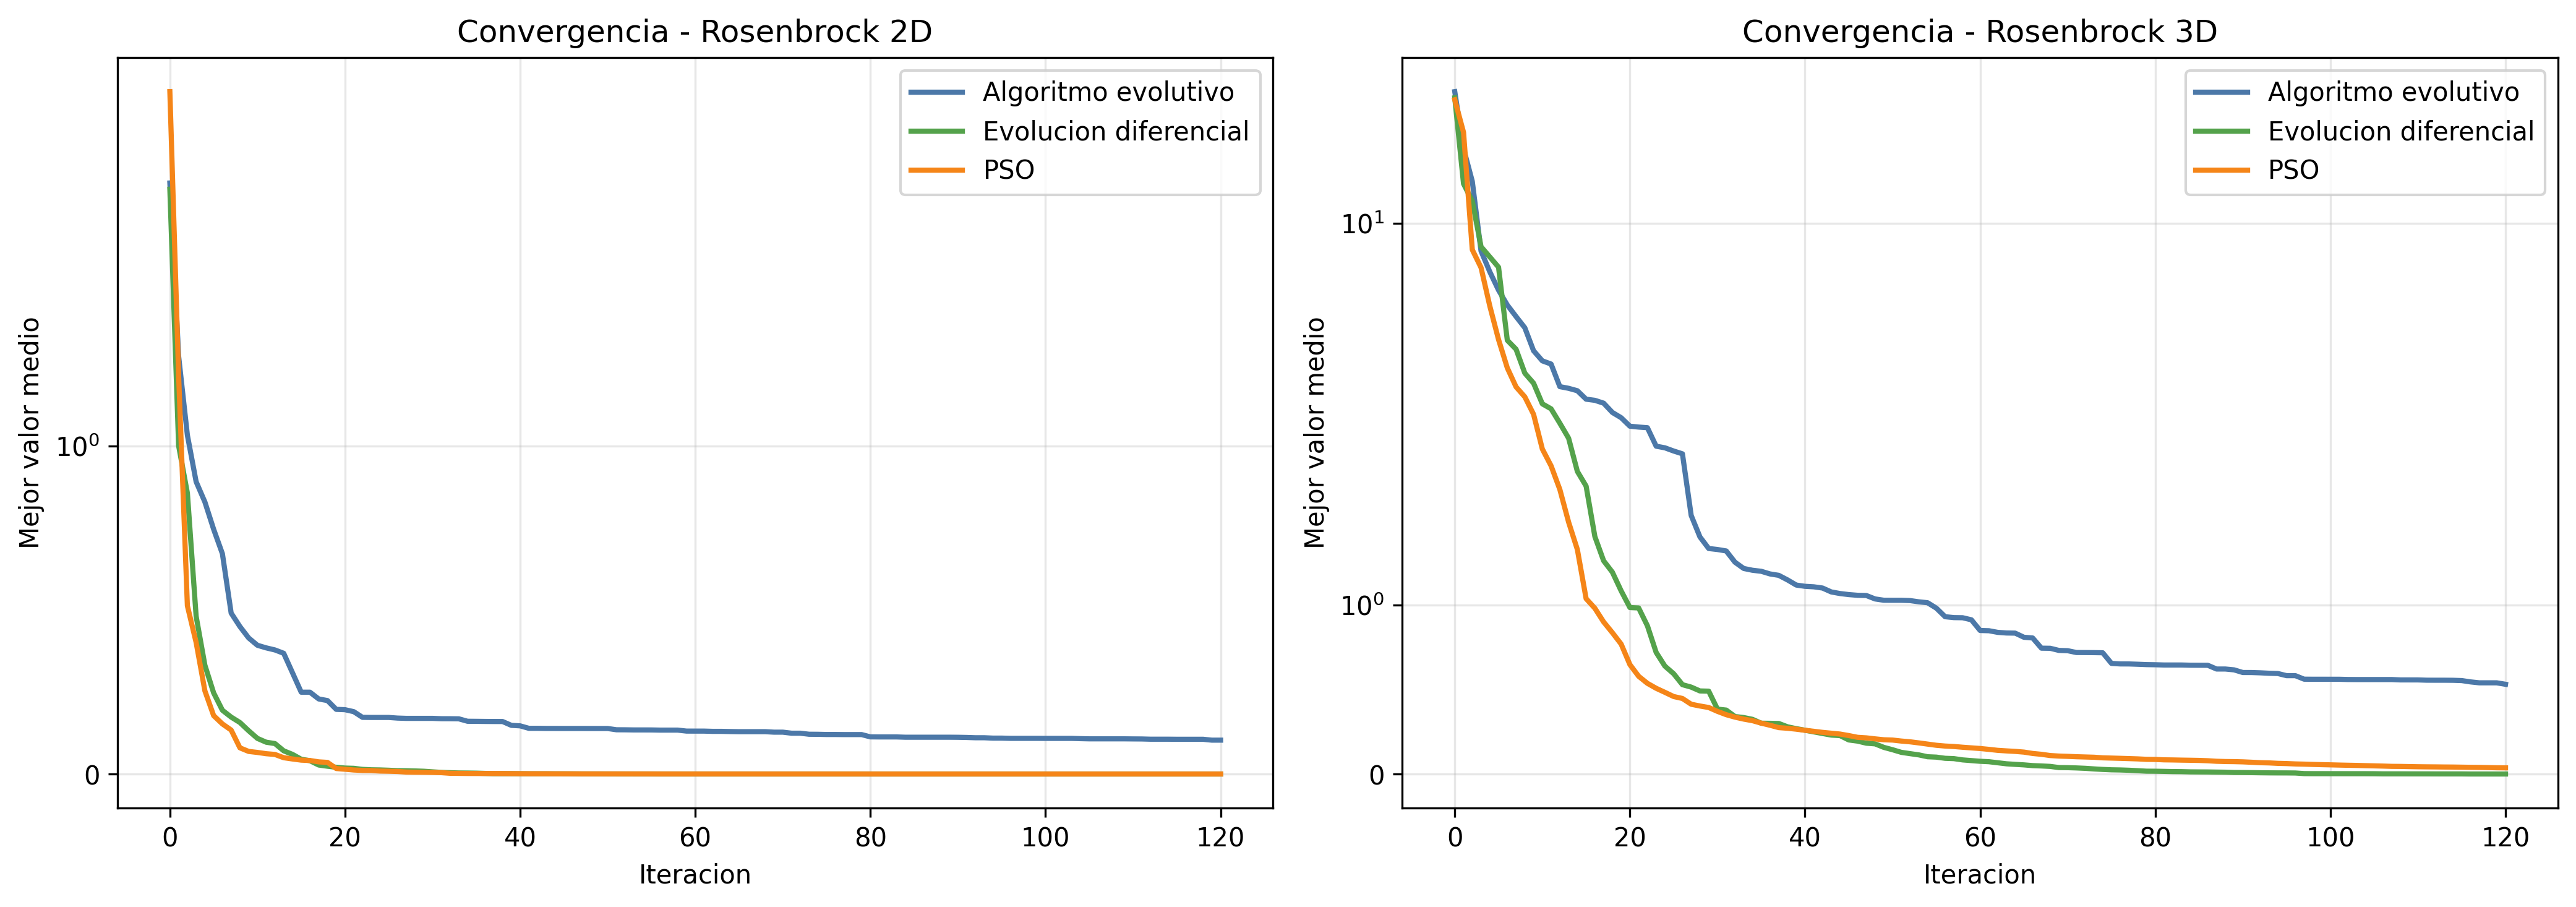
\includegraphics[keepaspectratio]{assets/numerica/heuristicos/images/rosenbrock/convergencia_rosenbrock_2d_3d.png}}

\paragraph{Función Schwefel}\label{funciuxf3n-schwefel-1}

\pandocbounded{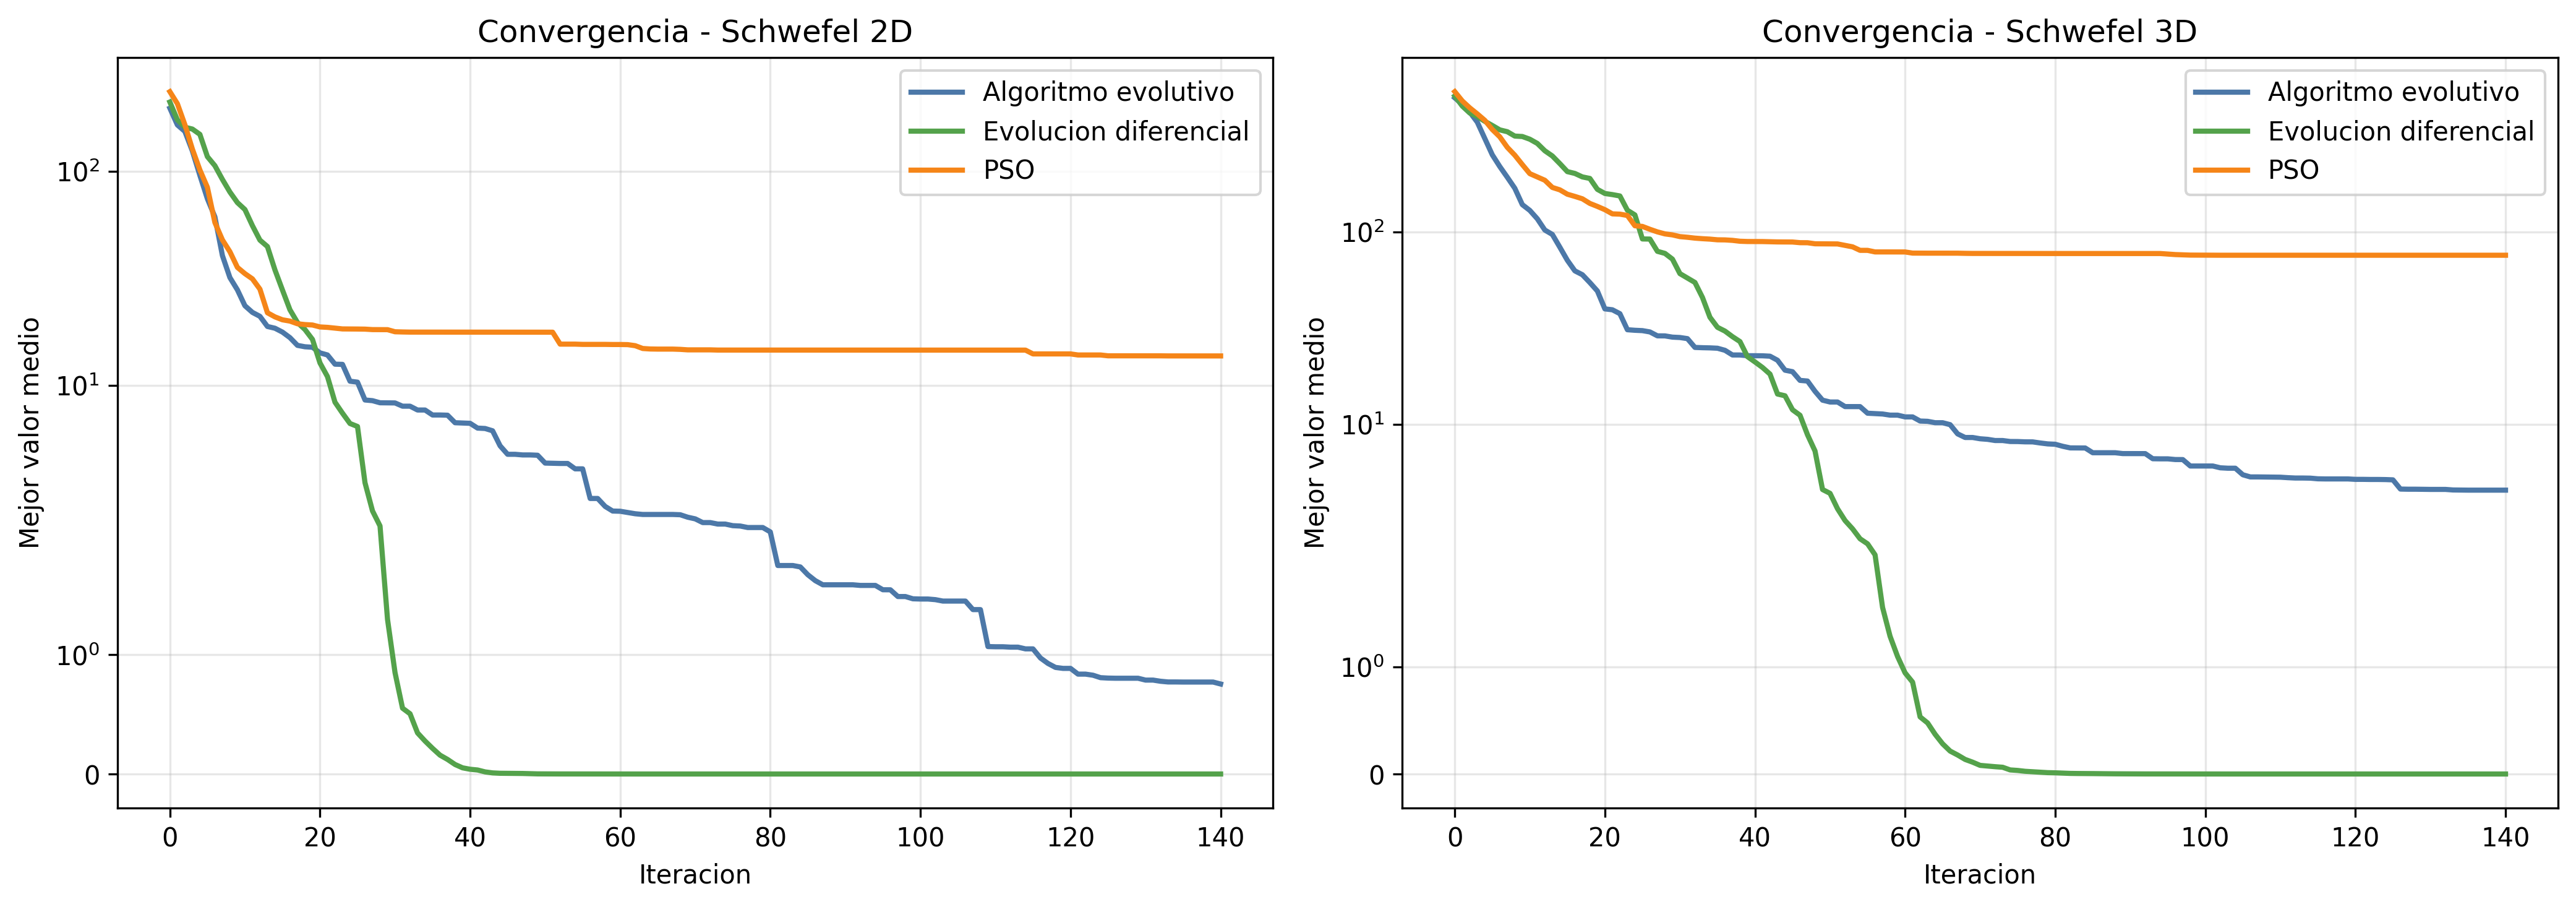
\includegraphics[keepaspectratio]{assets/numerica/heuristicos/images/schwefel/convergencia_schwefel_2d_3d.png}}

\paragraph{Función Rastrigin}\label{funciuxf3n-rastrigin-1}

\pandocbounded{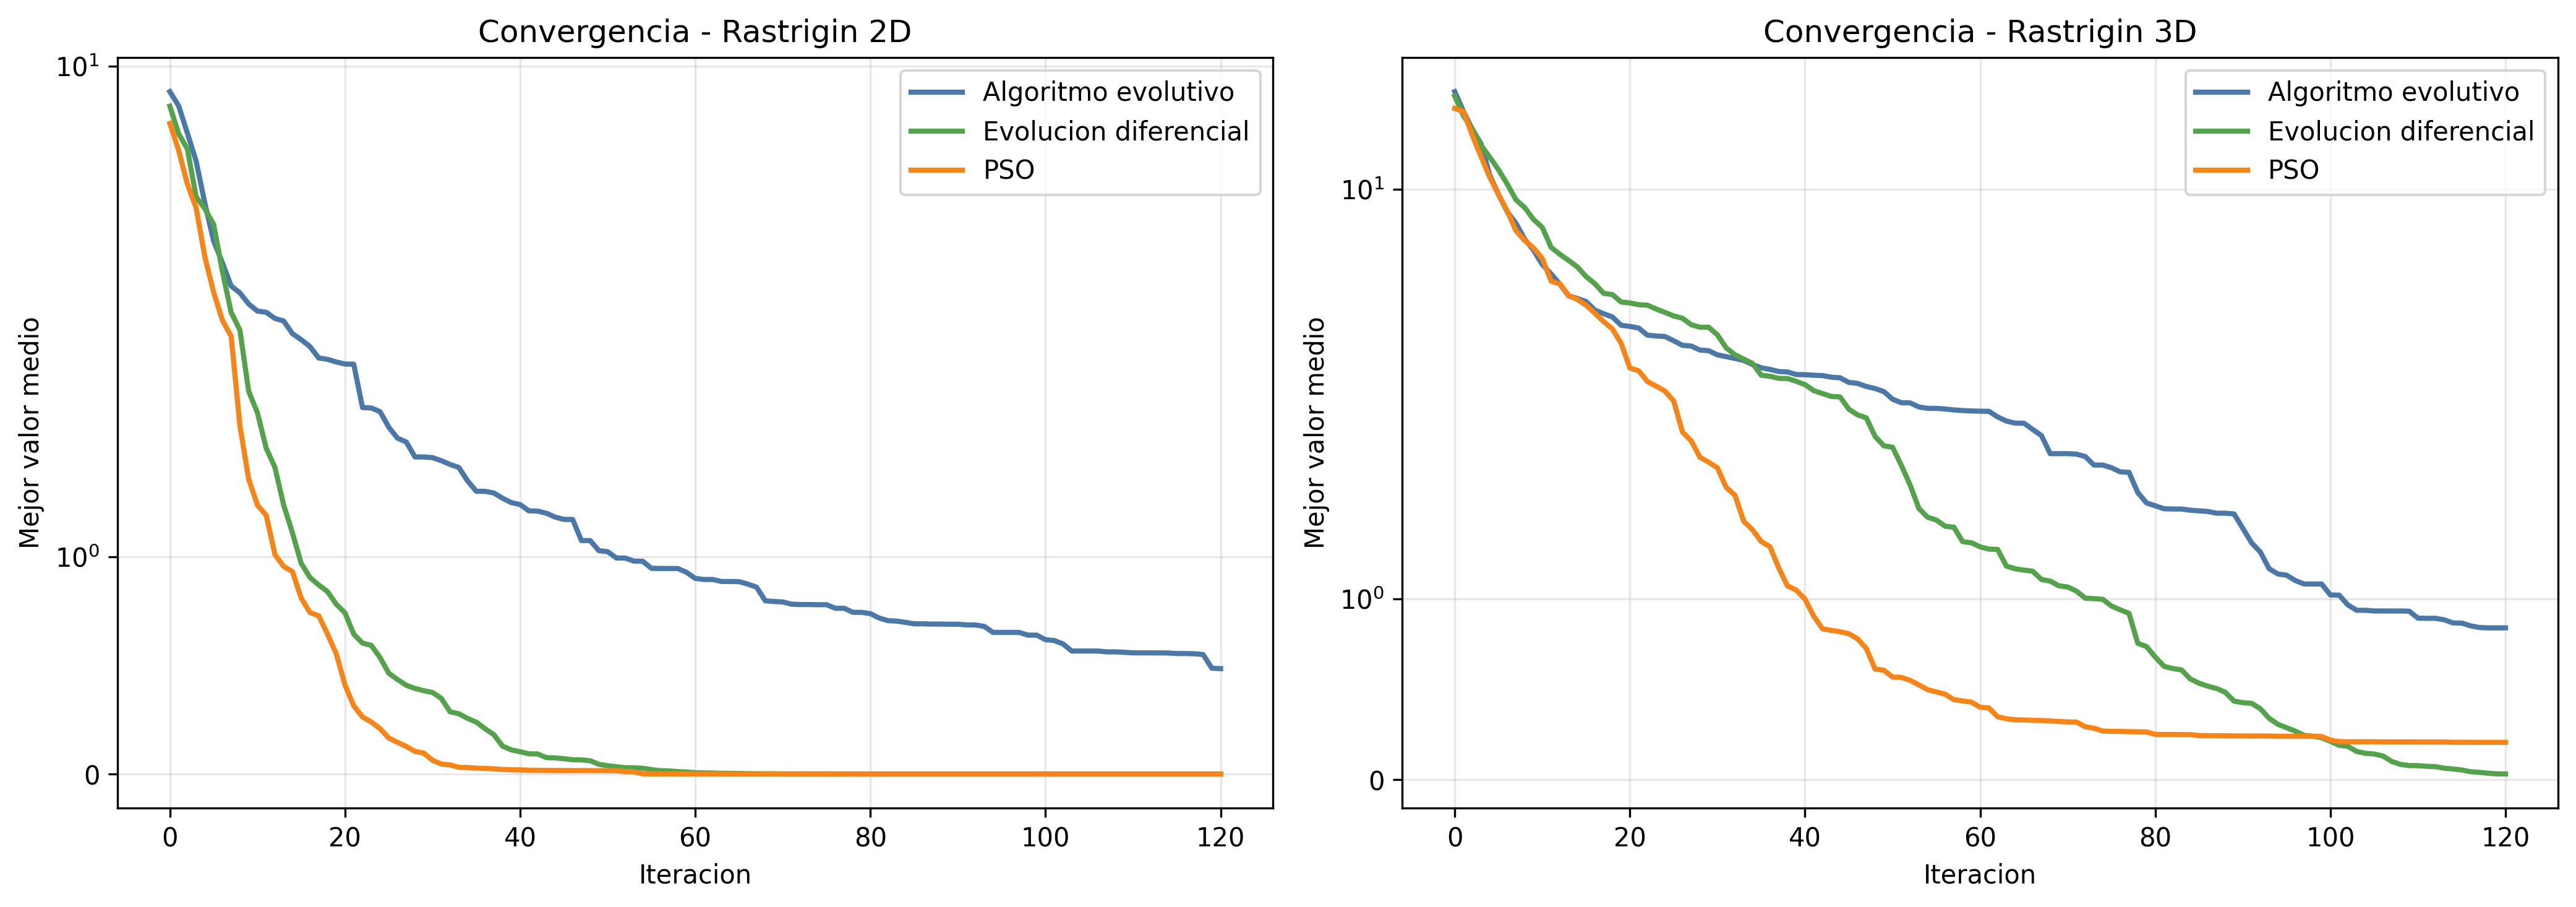
\includegraphics[keepaspectratio]{assets/numerica/heuristicos/images/rastrigin/convergencia_rastrigin_2d_3d.png}}

\paragraph{Función Griewank}\label{funciuxf3n-griewank-1}

\pandocbounded{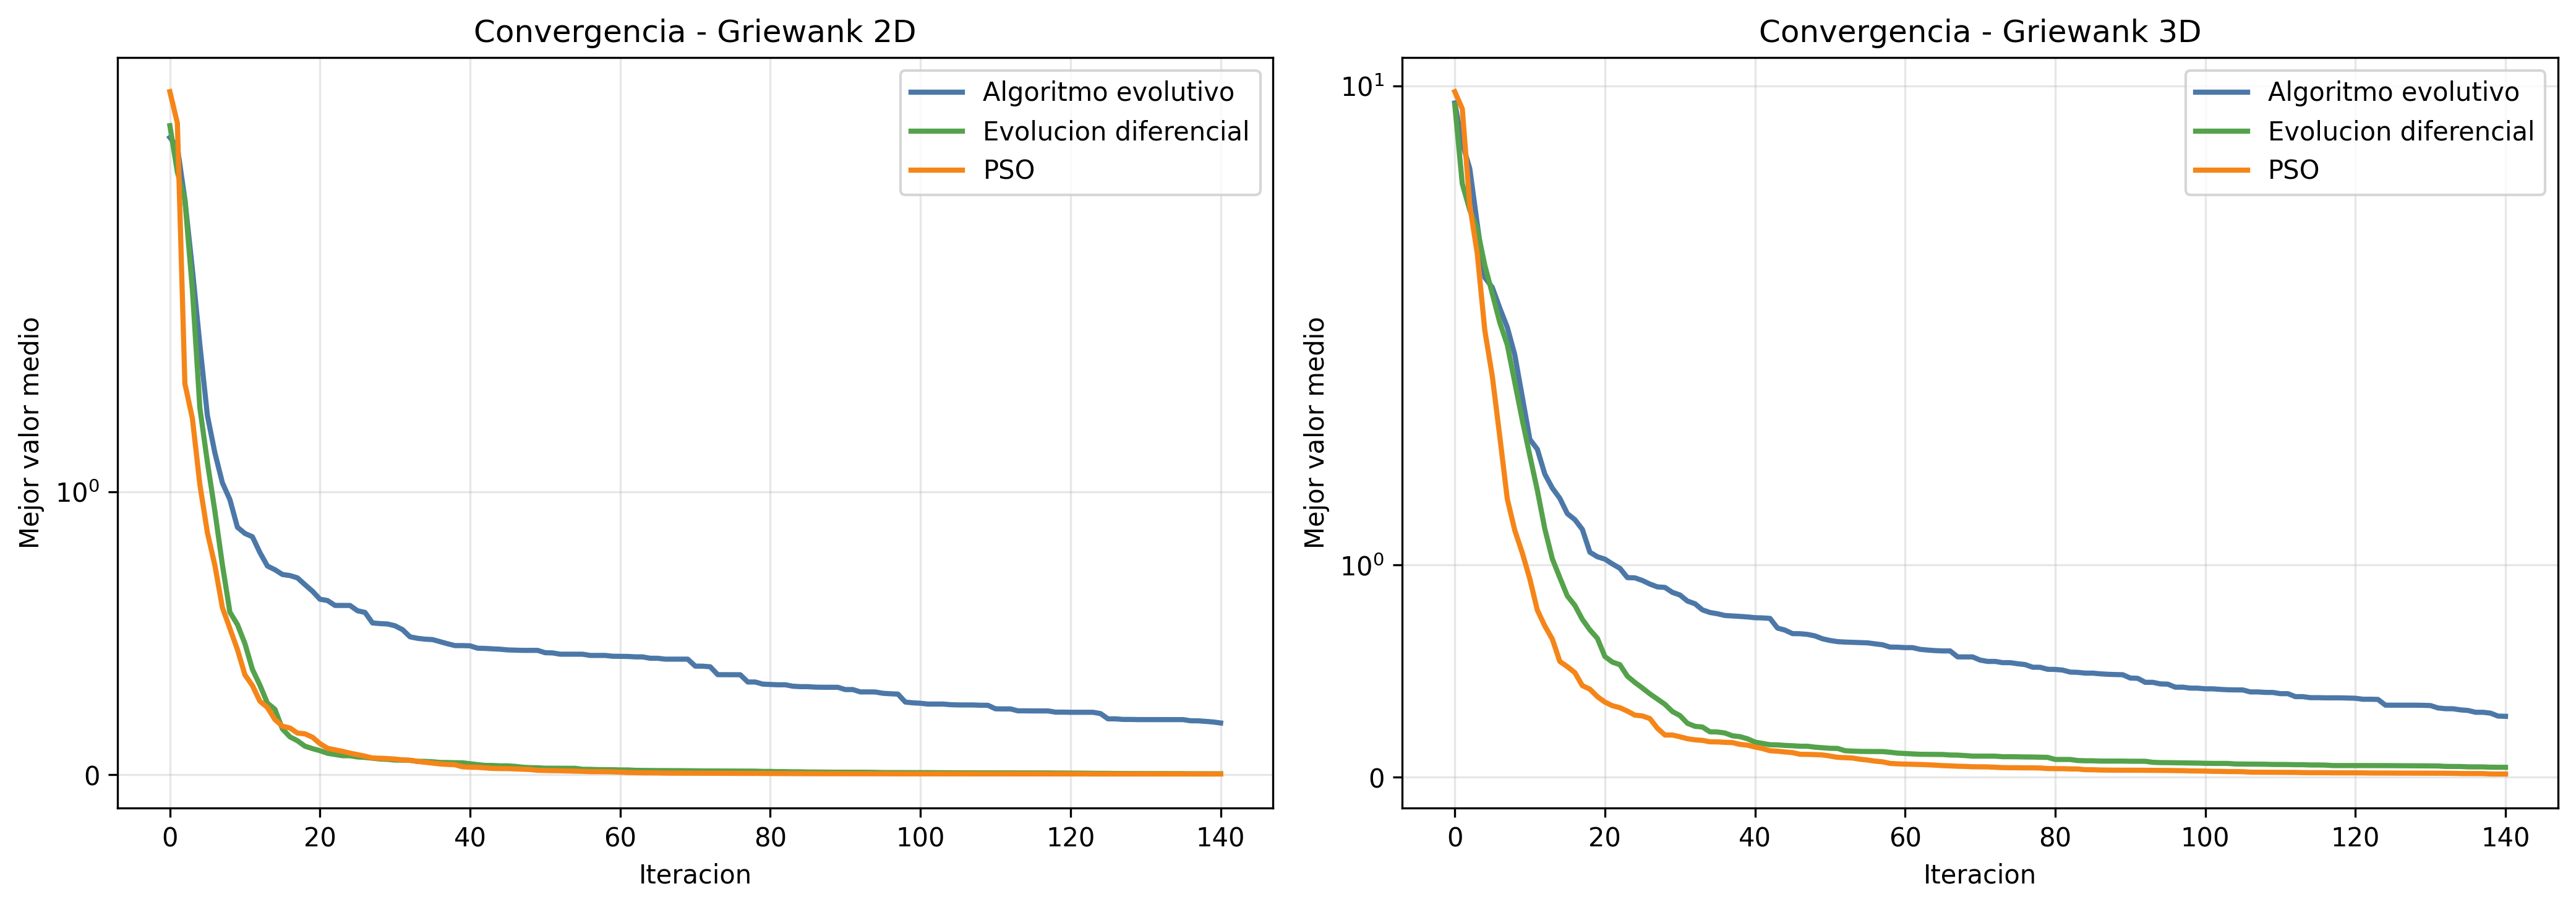
\includegraphics[keepaspectratio]{assets/numerica/heuristicos/images/griewank/convergencia_griewank_2d_3d.png}}

\paragraph{Función Goldstein-Price}\label{funciuxf3n-goldstein-price-1}

\pandocbounded{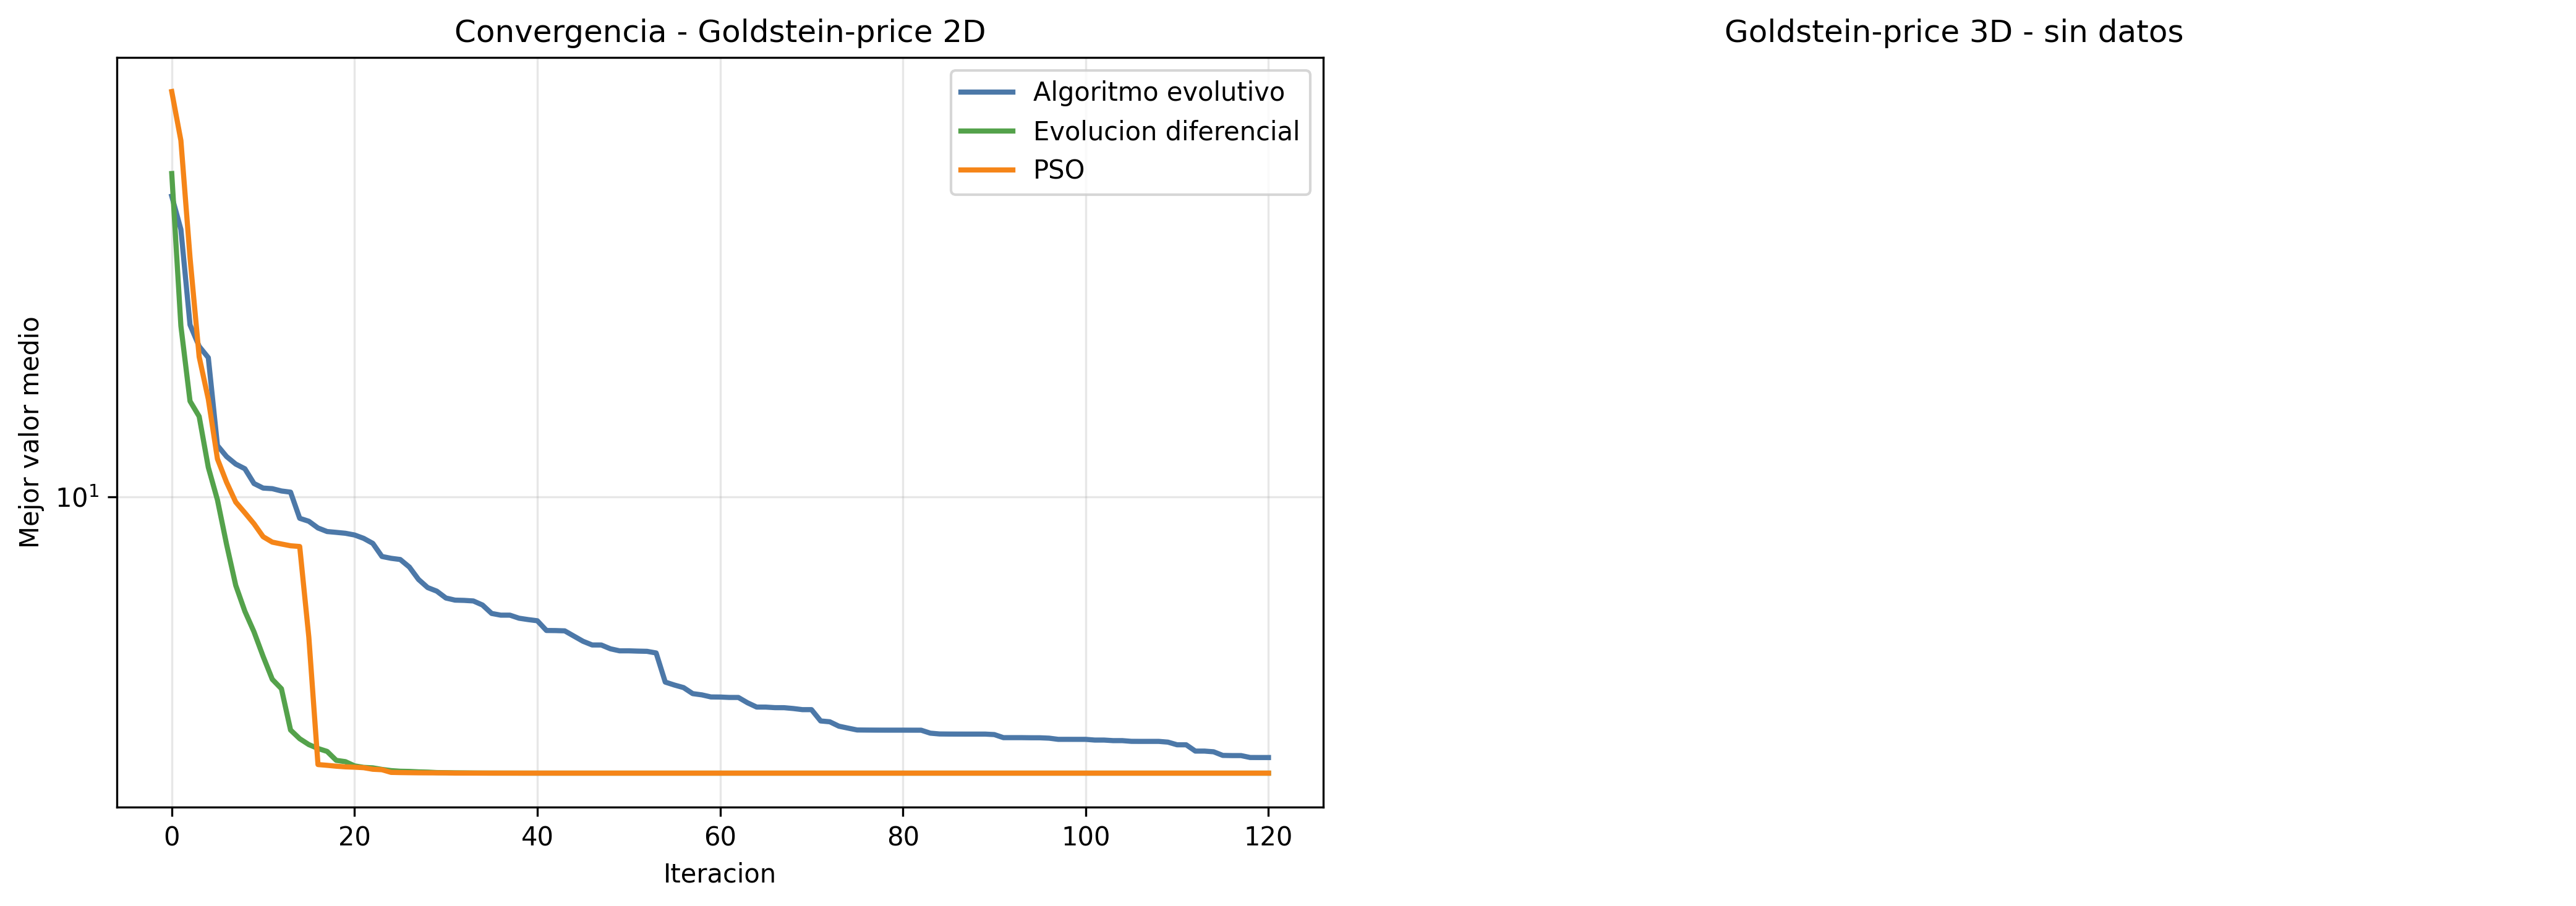
\includegraphics[keepaspectratio]{assets/numerica/heuristicos/images/goldstein-price/convergencia_goldstein-price_2d_3d.png}}

\paragraph{Función Six-Hump Camel}\label{funciuxf3n-six-hump-camel-2}

\pandocbounded{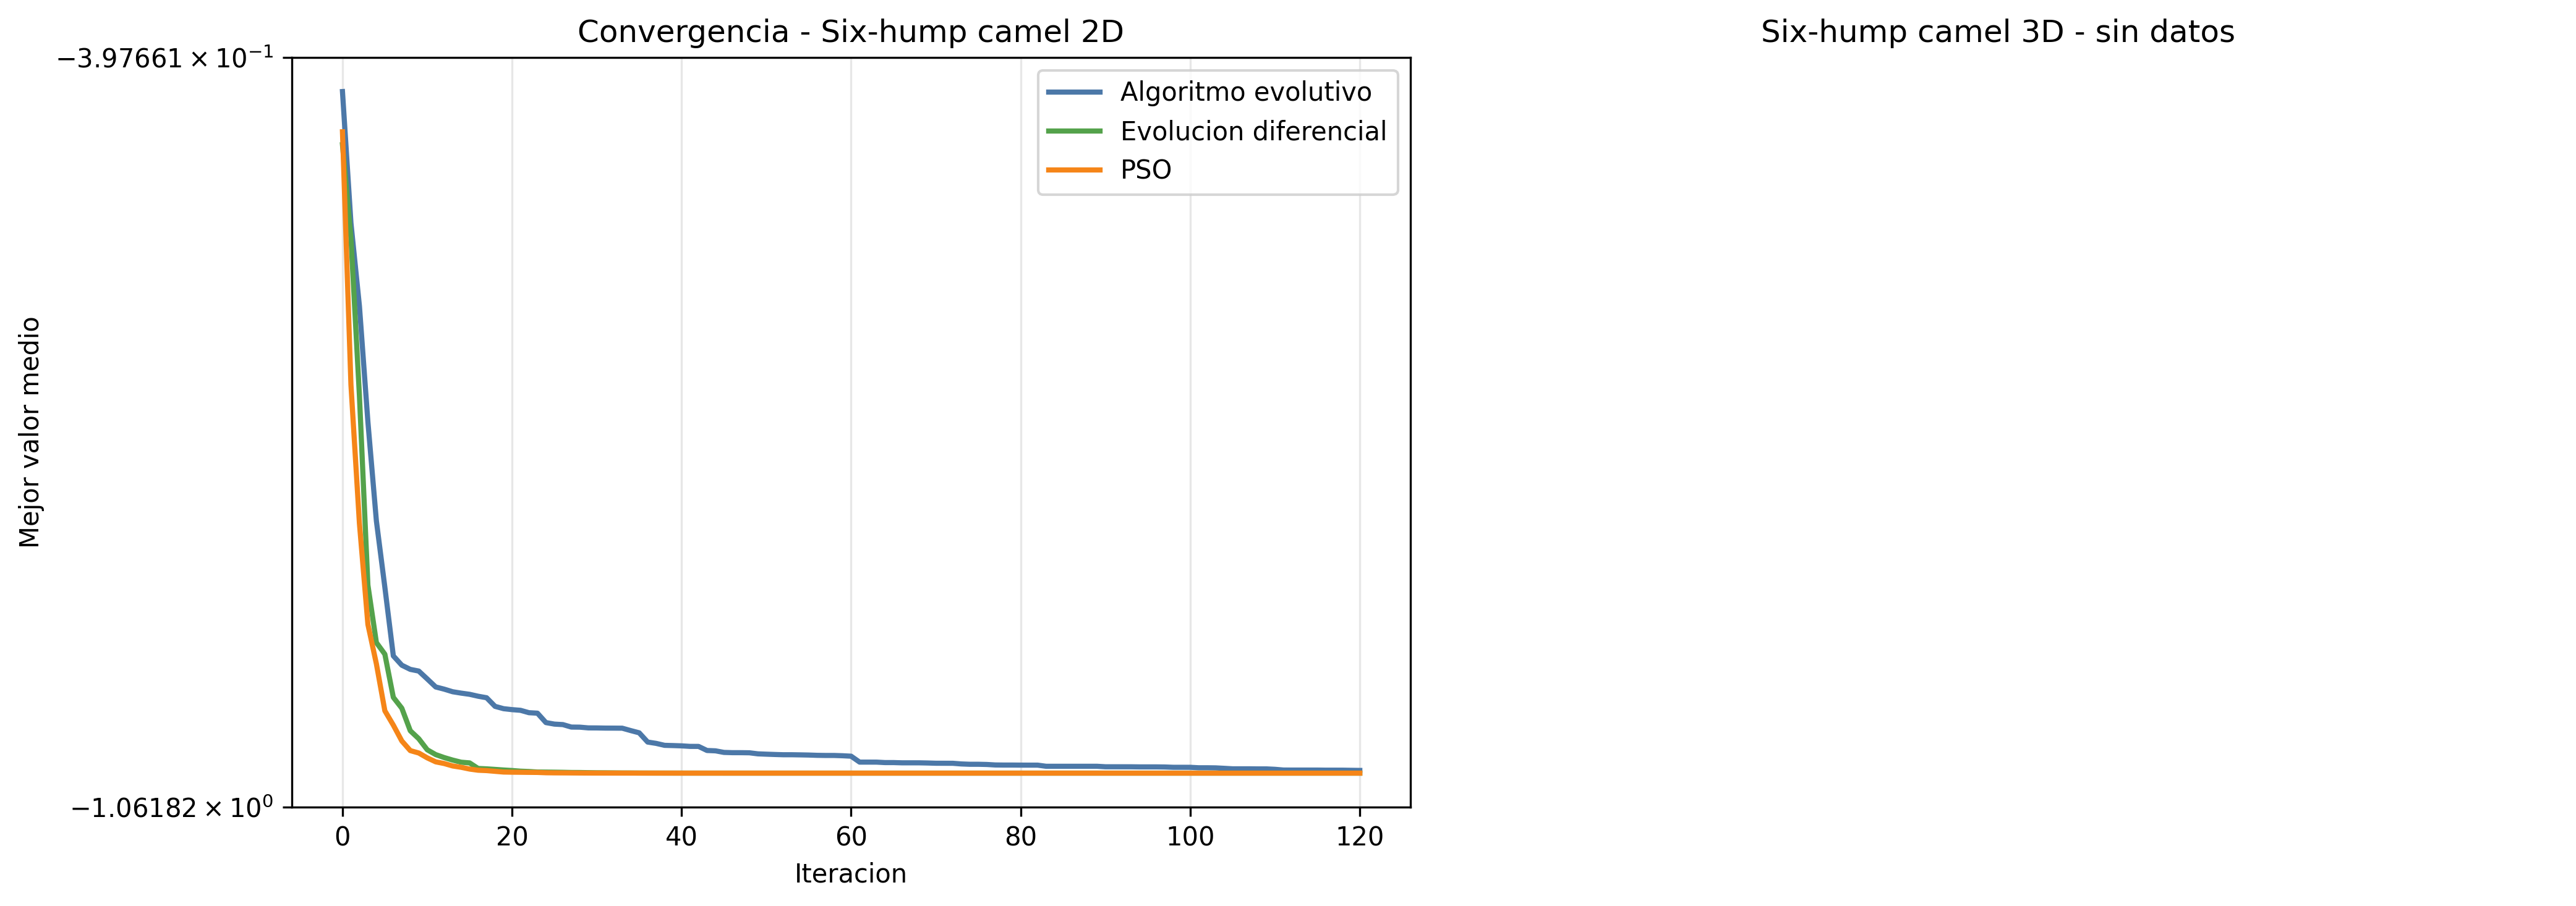
\includegraphics[keepaspectratio]{assets/numerica/heuristicos/images/six-hump camel/convergencia_six-hump camel_2d_3d.png}}

En general, las curvas muestran que \texttt{Evolución\ diferencial} es
el método más consistente, ya que converge con rapidez y suele terminar
más cerca del óptimo en la mayoría de las funciones. \texttt{PSO}
también presenta un muy buen desempeño, especialmente en
\texttt{Rastrigin}, \texttt{Griewank} y \texttt{Six-Hump\ Camel}, donde
desciende con rapidez y alcanza soluciones competitivas.

Por su parte, el \texttt{Algoritmo\ evolutivo} tiende a converger de
forma más lenta y en varios casos queda más alejado del mejor valor
final. En conjunto, los resultados refuerzan que
\texttt{Evolución\ diferencial} y \texttt{PSO} ofrecen el comportamiento
de convergencia más favorable dentro del estudio.

\paragraph{Conclusión Parcial}\label{conclusiuxf3n-parcial-1}

Los resultados obtenidos muestran que los métodos heurísticos evaluados
son capaces de aproximarse con buena precisión a los óptimos de varias
funciones de prueba, aunque su desempeño depende de la complejidad del
paisaje y de la dimensión del problema. En general,
\texttt{Evolución\ diferencial} fue el método más consistente, ya que
alcanzó valores promedio de \texttt{0.000000} en
\texttt{Rosenbrock\ 2D}, \texttt{Rastrigin\ 2D} y
\texttt{Goldstein-Price\ 2D}, además de \texttt{0.000025} en
\texttt{Schwefel\ 2D} y \texttt{0.000038} en \texttt{Schwefel\ 3D}.

Por su parte, \texttt{PSO} también presentó un comportamiento muy
competitivo, especialmente en \texttt{Griewank}, donde obtuvo el mejor
valor promedio con \texttt{0.002583} en \texttt{2D} y \texttt{0.009003}
en \texttt{3D}, y en \texttt{Six-Hump\ Camel\ 2D}, donde igualó el mejor
resultado con \texttt{-1.031628}. En contraste, el
\texttt{Algoritmo\ evolutivo} mostró un desempeño más variable, con
promedios más altos como \texttt{0.527946} en \texttt{Rosenbrock\ 3D},
\texttt{0.818432} en \texttt{Rastrigin\ 3D} y \texttt{4.713732} en
\texttt{Schwefel\ 3D}.

Además, se observó que el aumento de dimensionalidad tiende a hacer más
difícil la búsqueda del óptimo. Por ejemplo, en \texttt{Rosenbrock} el
mejor promedio pasó de \texttt{0.000000} en \texttt{2D} a
\texttt{0.000242} en \texttt{3D}, en \texttt{Rastrigin} de
\texttt{0.000000} a \texttt{0.038206}, y en \texttt{Griewank} de
\texttt{0.002583} a \texttt{0.009003}. Esto confirma que la complejidad
del problema influye directamente en la estabilidad y eficacia de los
métodos empleados.

En conjunto, el análisis confirma que los métodos heurísticos son una
alternativa efectiva para problemas de optimización no lineal y
multimodal, pero también evidencia que no existe un único enfoque
universalmente superior para todos los casos. Aun así, dentro de este
estudio, \texttt{Evolución\ diferencial} se perfila como la opción más
robusta y equilibrada, mientras que \texttt{PSO} destaca en funciones
específicas donde alcanza resultados iguales o incluso mejores.

\subsection{Comparación final entre
métodos}\label{comparaciuxf3n-final-entre-muxe9todos}

Esta página está pensada para comparar los métodos \textbf{dentro del
mismo caso}, no entre funciones distintas. La comparación correcta es:

\begin{itemize}
\tightlist
\item
  \texttt{Rosenbrock\ 2D\ y\ 3D}: comparación entre descenso por
  gradiente, algoritmo evolutivo, PSO y evolución diferencial
  \pandocbounded{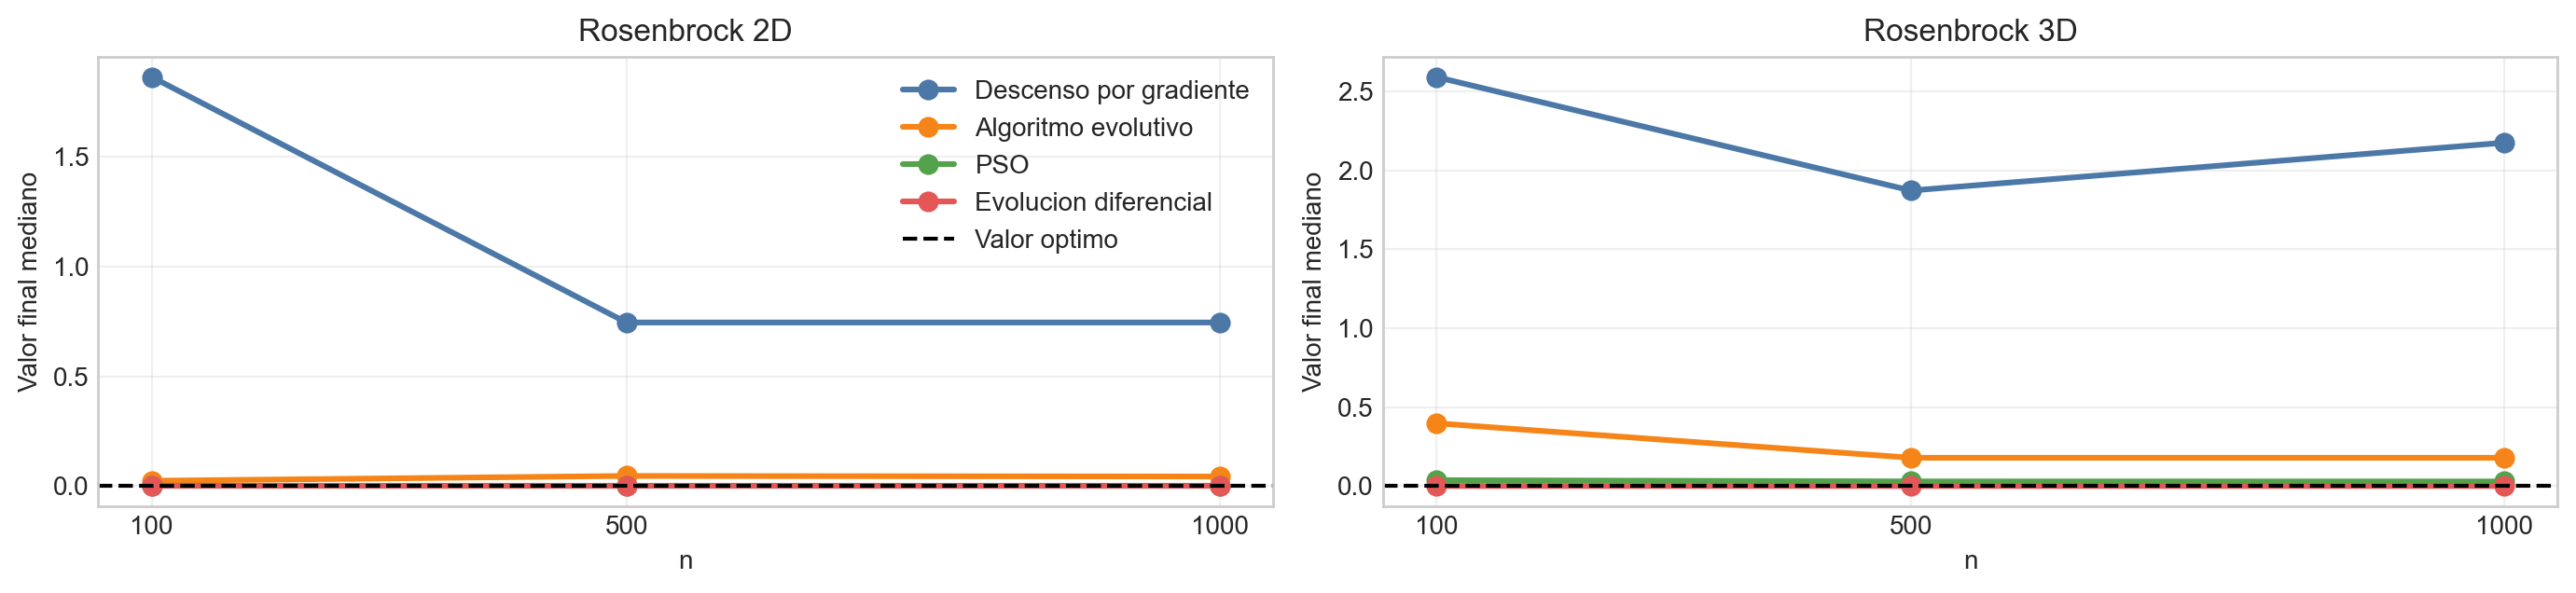
\includegraphics[keepaspectratio]{assets/comparacion/rosenbrock_lineas_por_n.png}}
  \pandocbounded{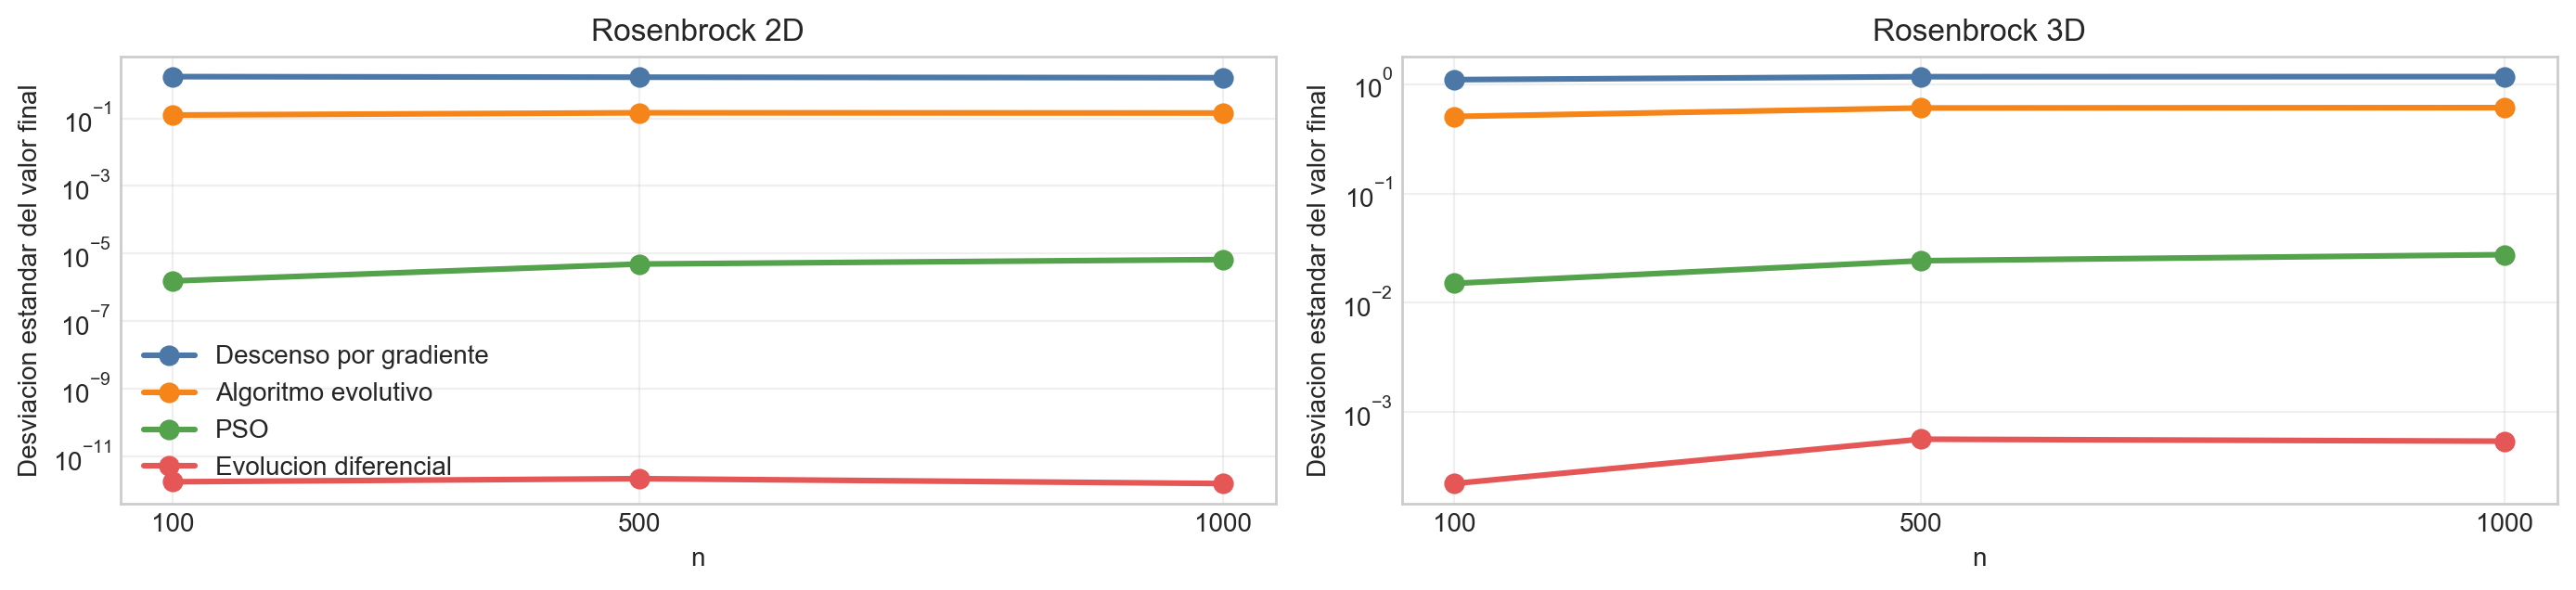
\includegraphics[keepaspectratio]{assets/comparacion/rosenbrock_lineas_desviacion_por_n.png}}
\end{itemize}

En la función Rosenbrock, PSO y, especialmente, Evolución diferencial
muestran el mejor desempeño, ya que alcanzan valores finales medianos
muy cercanos al óptimo tanto en 2D como en 3D y, además, presentan una
variabilidad muy baja.

El Algoritmo evolutivo se ubica en un nivel intermedio: mejora con
claridad frente a Descenso por gradiente, pero todavía queda algo más
alejado del valor óptimo, sobre todo en 3D. En cambio, Descenso por
gradiente registra los valores finales más altos y una mayor dispersión,
por lo que resulta ser el método menos preciso y menos estable en esta
comparación.

\begin{itemize}
\tightlist
\item
  \texttt{Rastrigin\ 2D\ y\ 3D}: gradiente vs EA vs PSO vs DE
  \pandocbounded{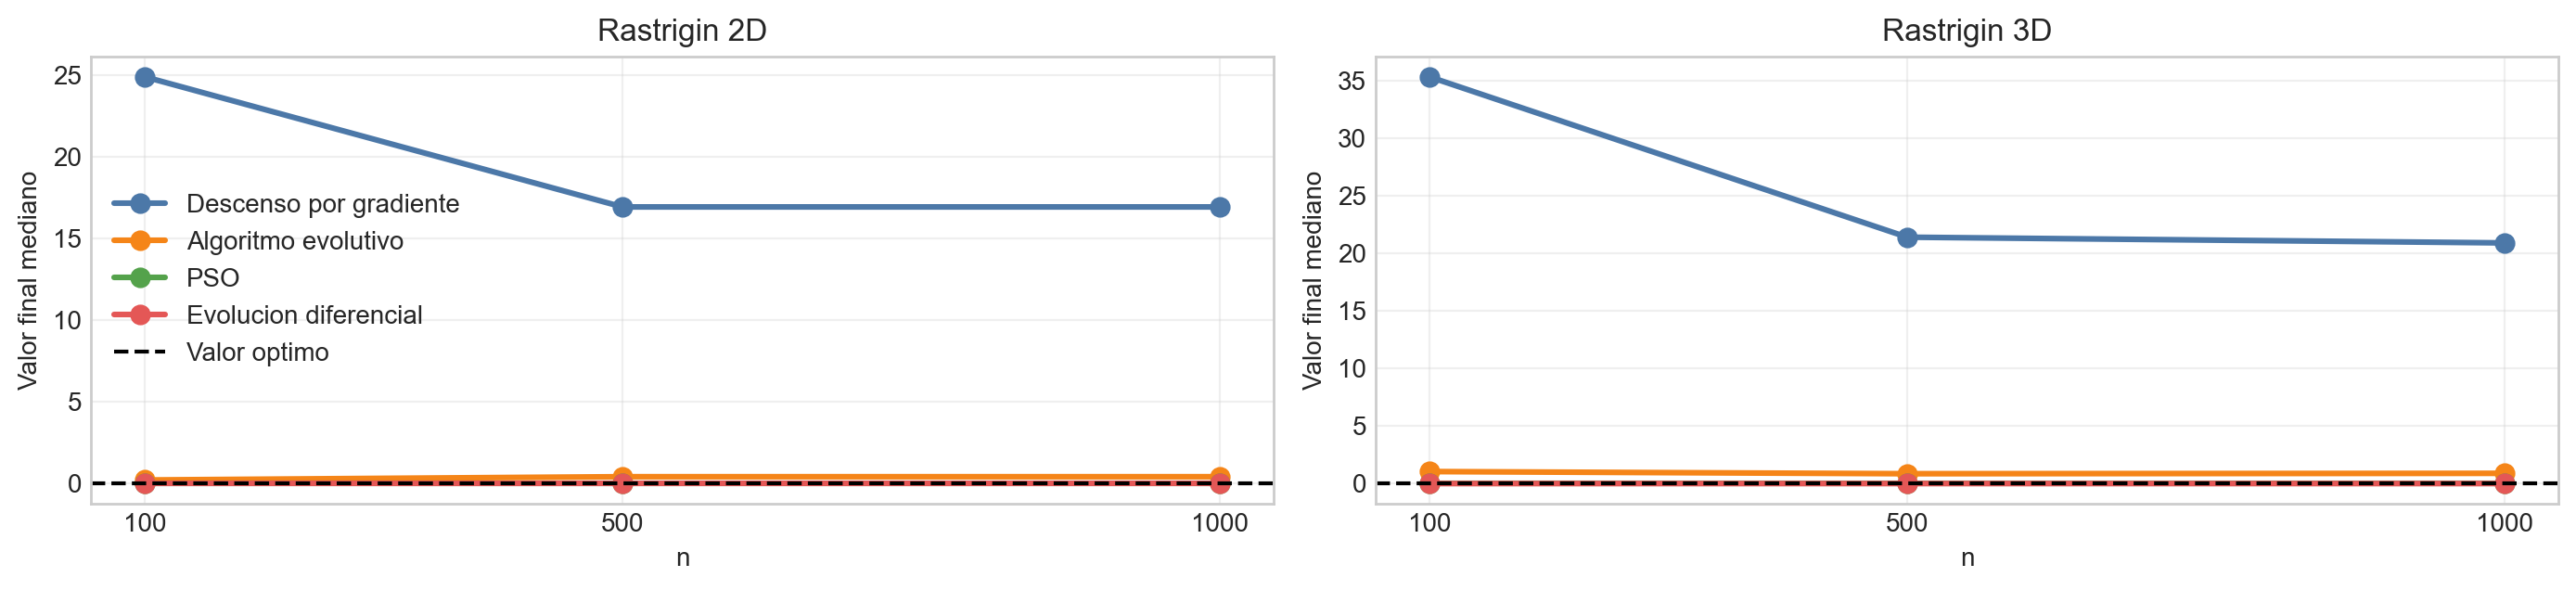
\includegraphics[keepaspectratio]{assets/comparacion/rastrigin_lineas_por_n.png}}
  \pandocbounded{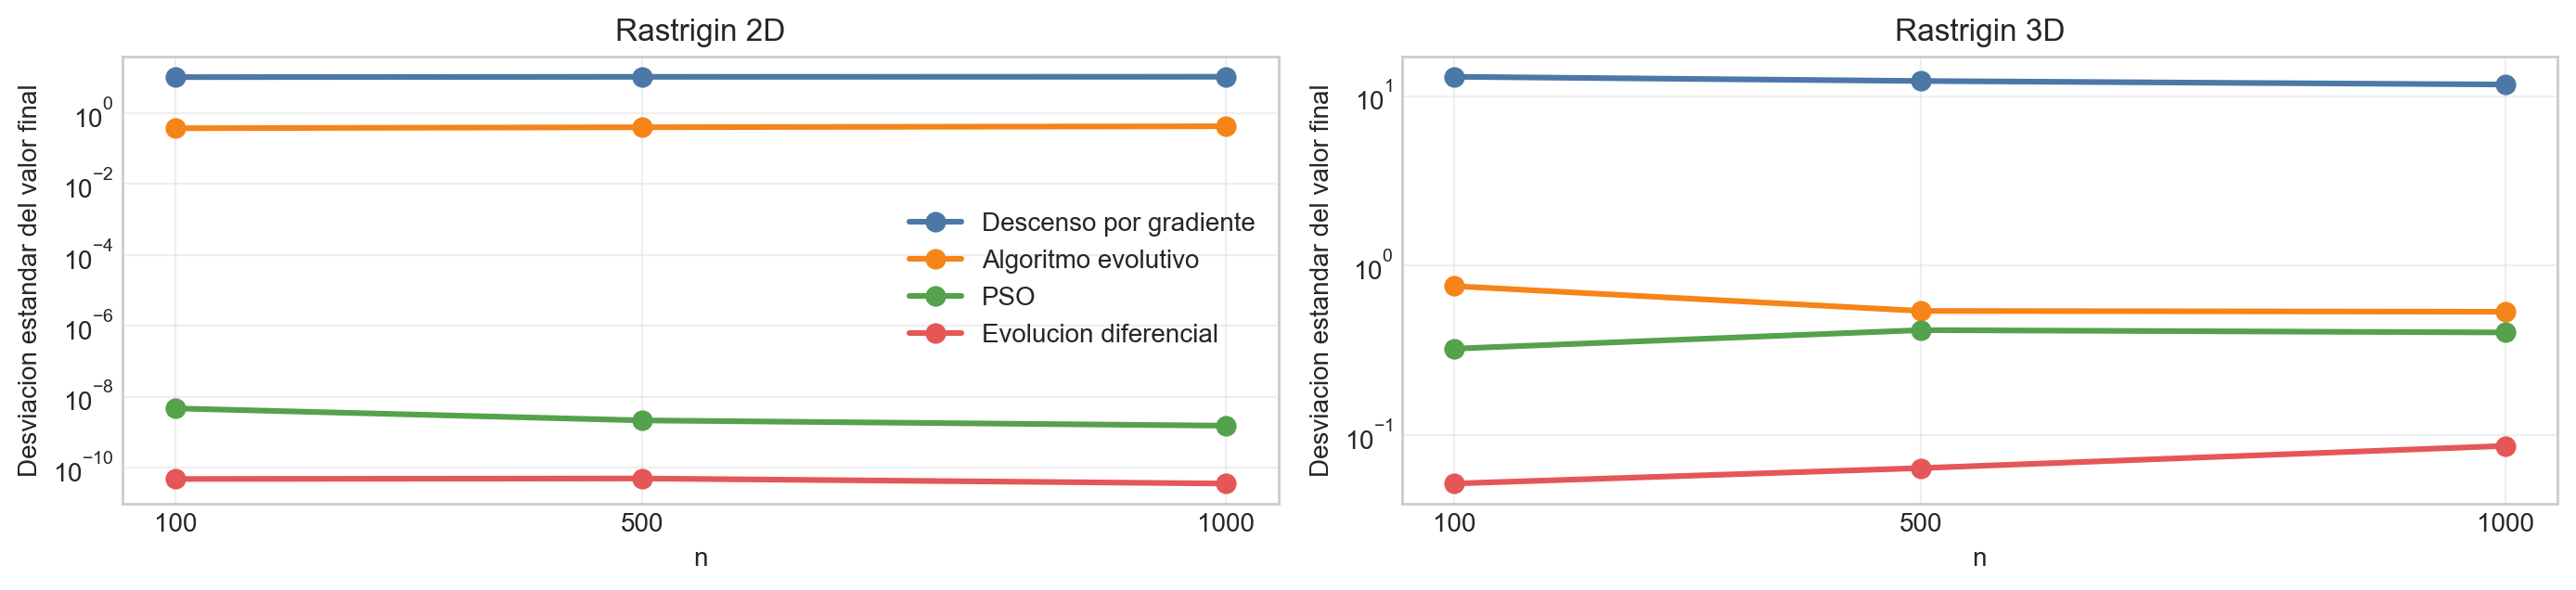
\includegraphics[keepaspectratio]{assets/comparacion/rastrigin_lineas_desviacion_por_n.png}}
\end{itemize}

Para la función Rastrigin, la diferencia entre métodos es aún más
evidente. Evolución diferencial y PSO vuelven a destacar como las
alternativas más efectivas, al mantener valores finales muy próximos al
óptimo y desviaciones reducidas, incluso cuando aumenta la dimensión del
problema.

El Algoritmo evolutivo ofrece un comportamiento aceptable, pero sigue
mostrando una brecha frente a los mejores métodos. Por su parte,
Descenso por gradiente presenta los peores resultados, con valores
finales claramente más altos y una variabilidad mayor, lo que indica
menor capacidad para converger de forma precisa en esta función.

\begin{itemize}
\tightlist
\item
  \texttt{Schwefel\ 2D\ y\ 3D}: gradiente vs EA vs PSO vs DE
  \pandocbounded{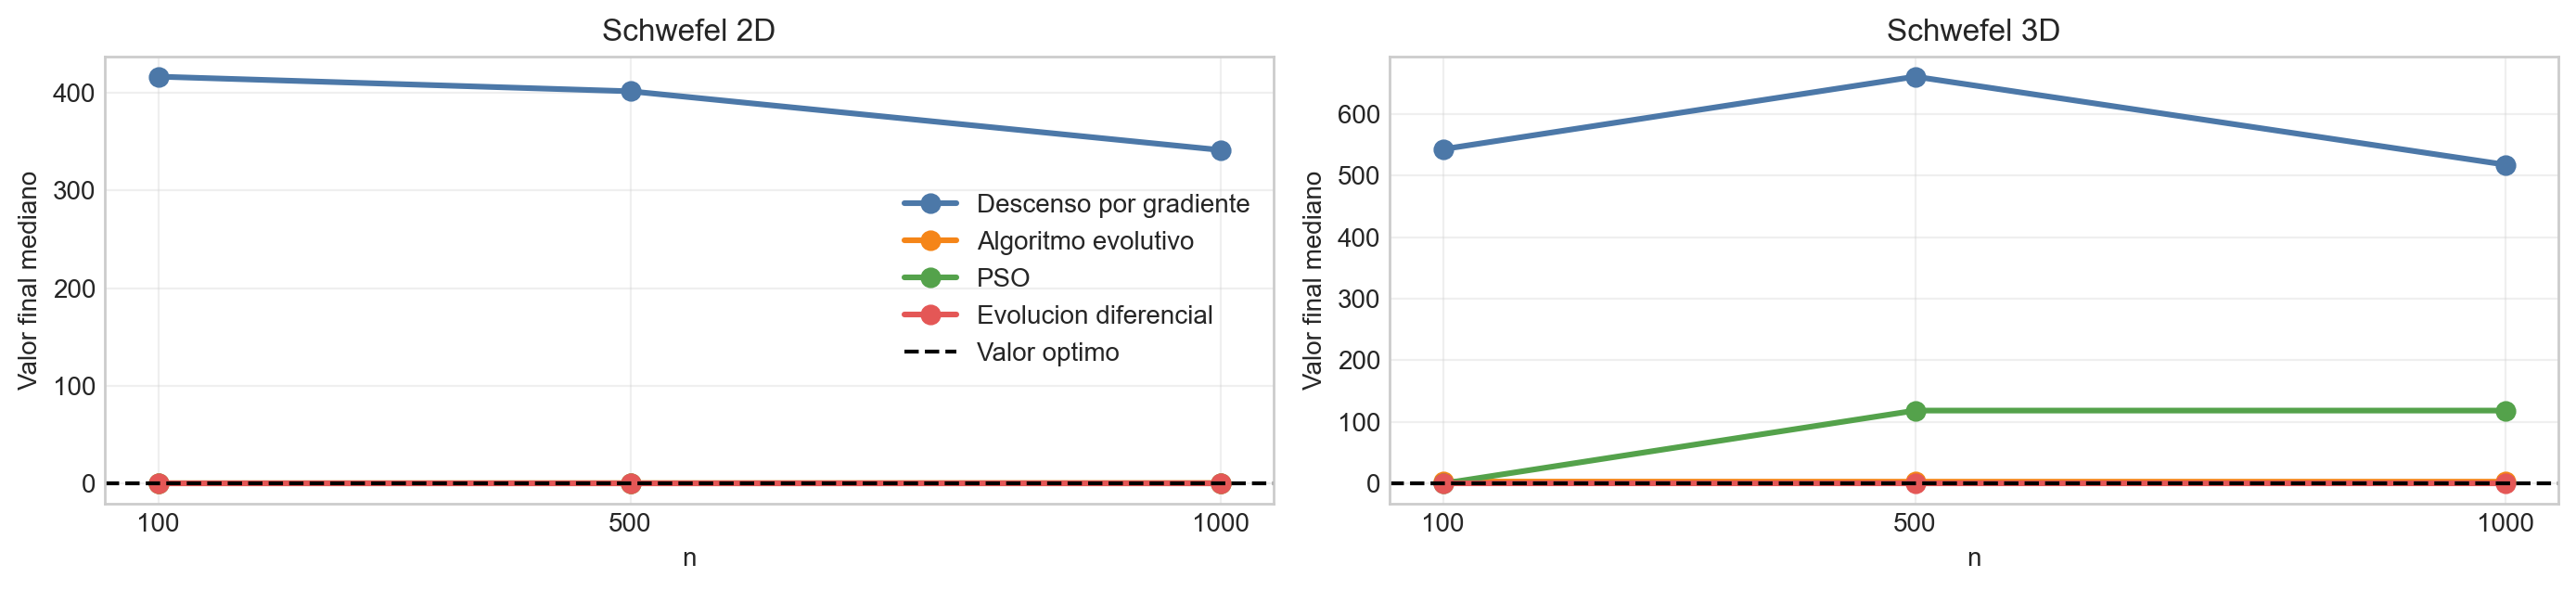
\includegraphics[keepaspectratio]{assets/comparacion/schwefel_lineas_por_n.png}}
  \pandocbounded{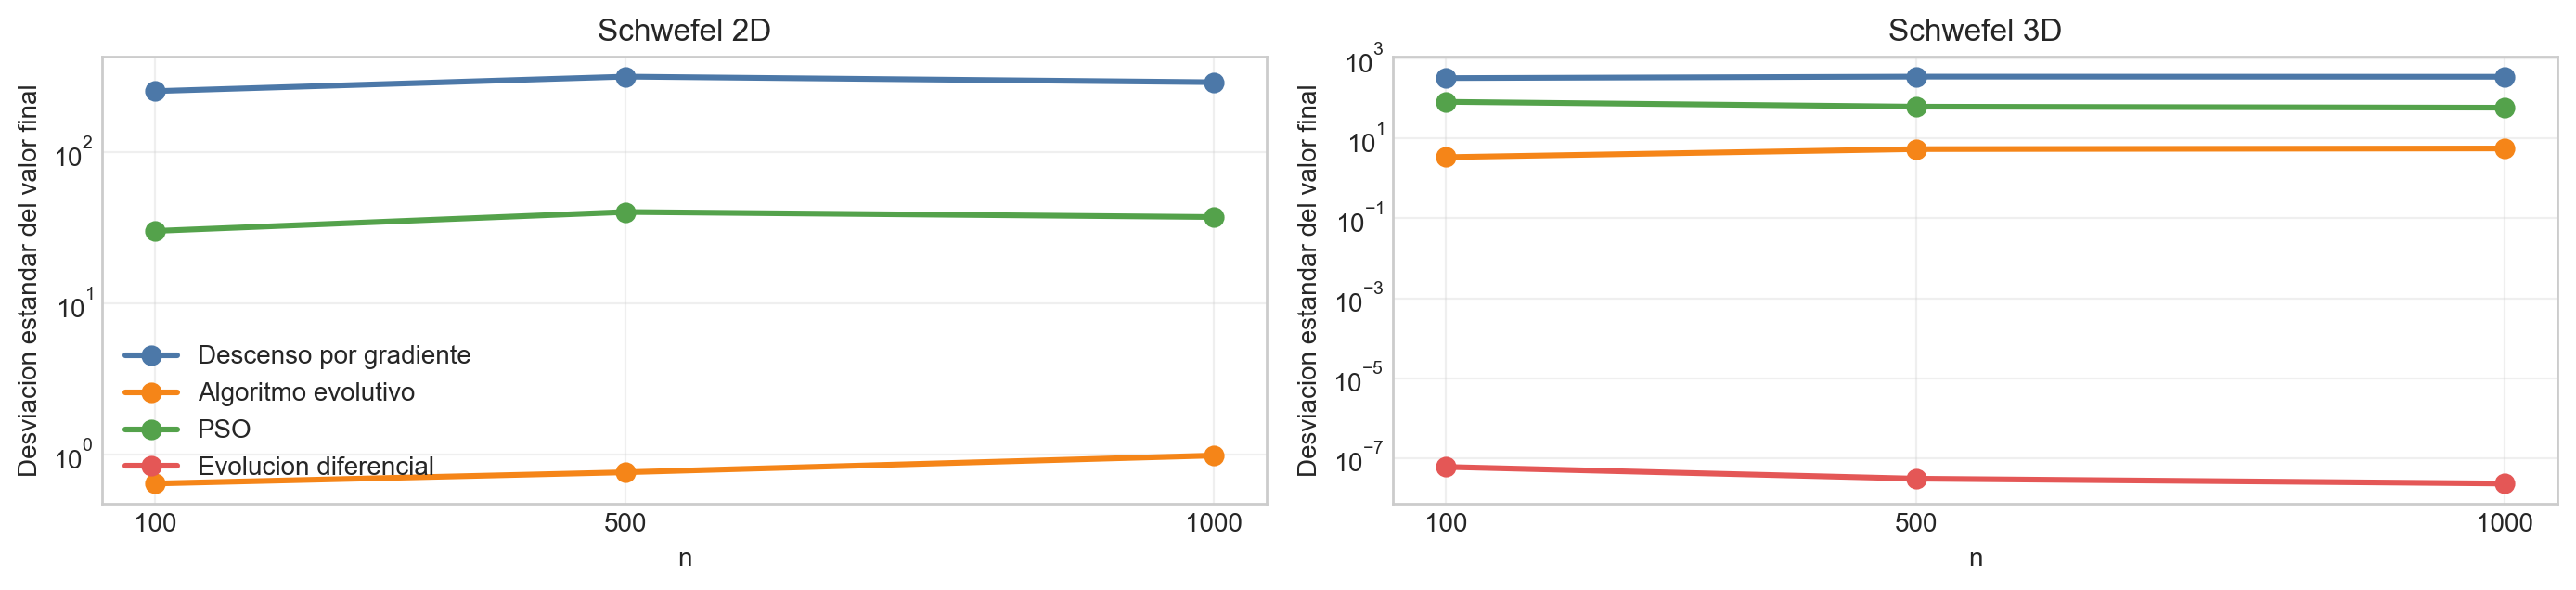
\includegraphics[keepaspectratio]{assets/comparacion/schwefel_lineas_desviacion_por_n.png}}
\end{itemize}

En la función Schwefel, \texttt{Evolución\ diferencial} es el método más
sólido en ambas dimensiones, ya que mantiene valores finales medianos
prácticamente sobre el óptimo y, además, exhibe la menor desviación
entre todos los enfoques. El \texttt{Algoritmo\ evolutivo} también
presenta un muy buen comportamiento, con resultados cercanos al óptimo y
una variabilidad bastante baja, aunque sin alcanzar la consistencia de
\texttt{DE}. En contraste, \texttt{PSO} y, sobre todo,
\texttt{Descenso\ por\ gradiente} muestran un desempeño más débil:
\texttt{PSO} se deteriora con claridad en 3D, mientras que
\texttt{Descenso\ por\ gradiente} conserva los valores finales más altos
y la mayor dispersión, por lo que resulta el método menos preciso y
menos estable en esta comparación.

\begin{itemize}
\tightlist
\item
  \texttt{Griewank\ 2D\ y\ 3D}: gradiente vs EA vs PSO vs DE
  \pandocbounded{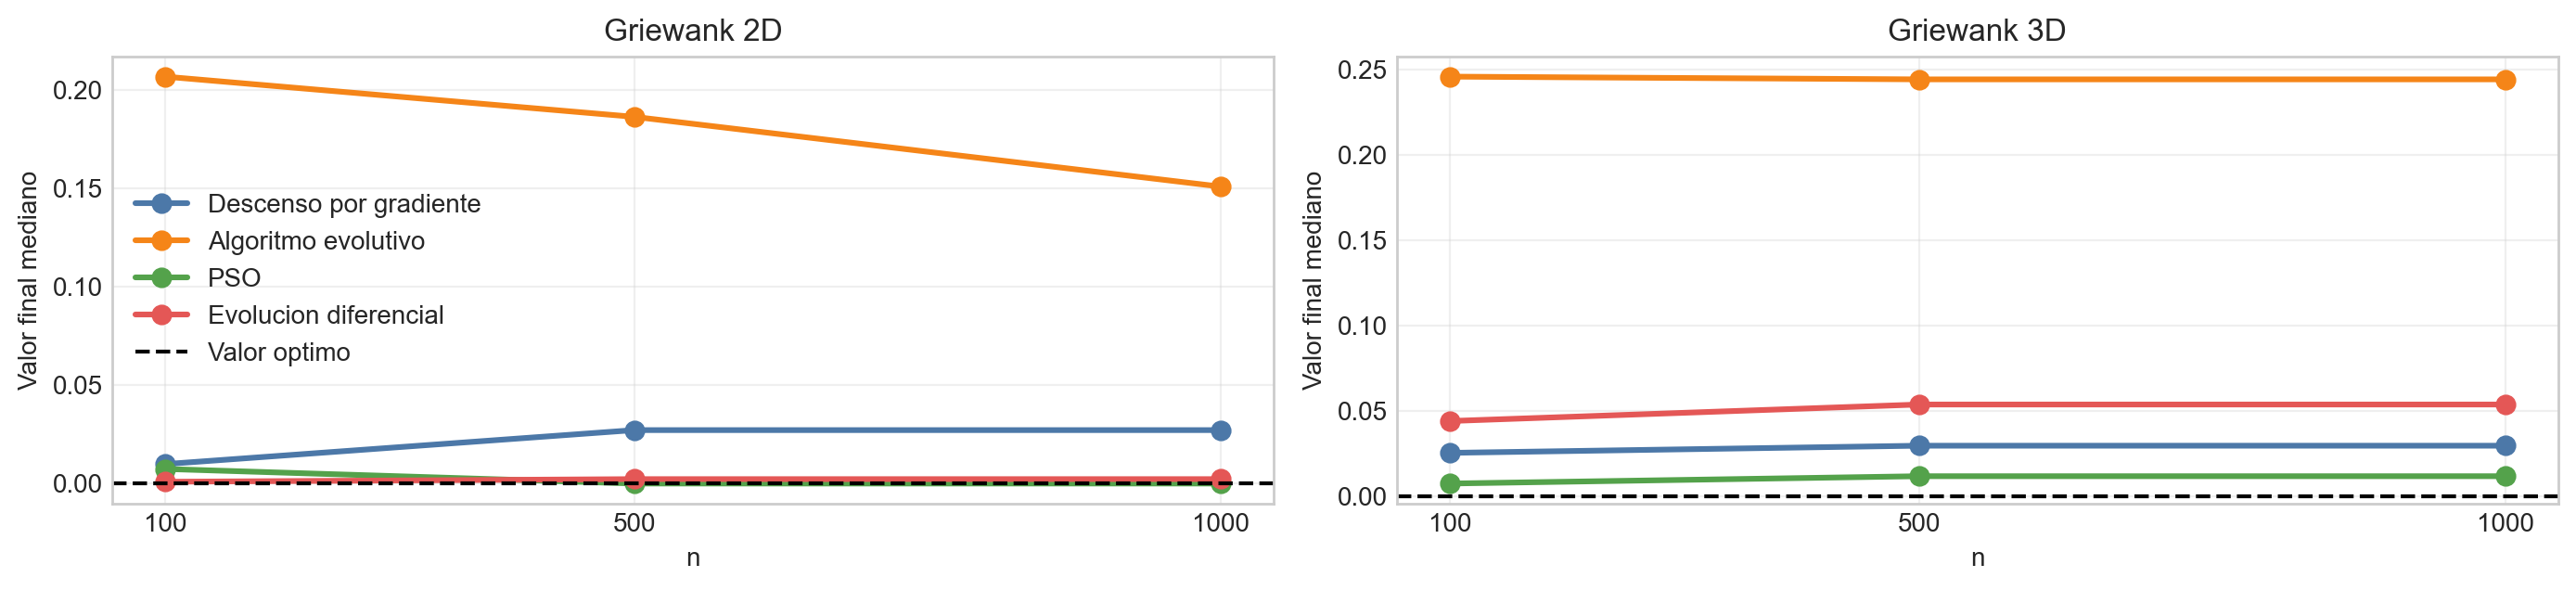
\includegraphics[keepaspectratio]{assets/comparacion/griewank_lineas_por_n.png}}
  \pandocbounded{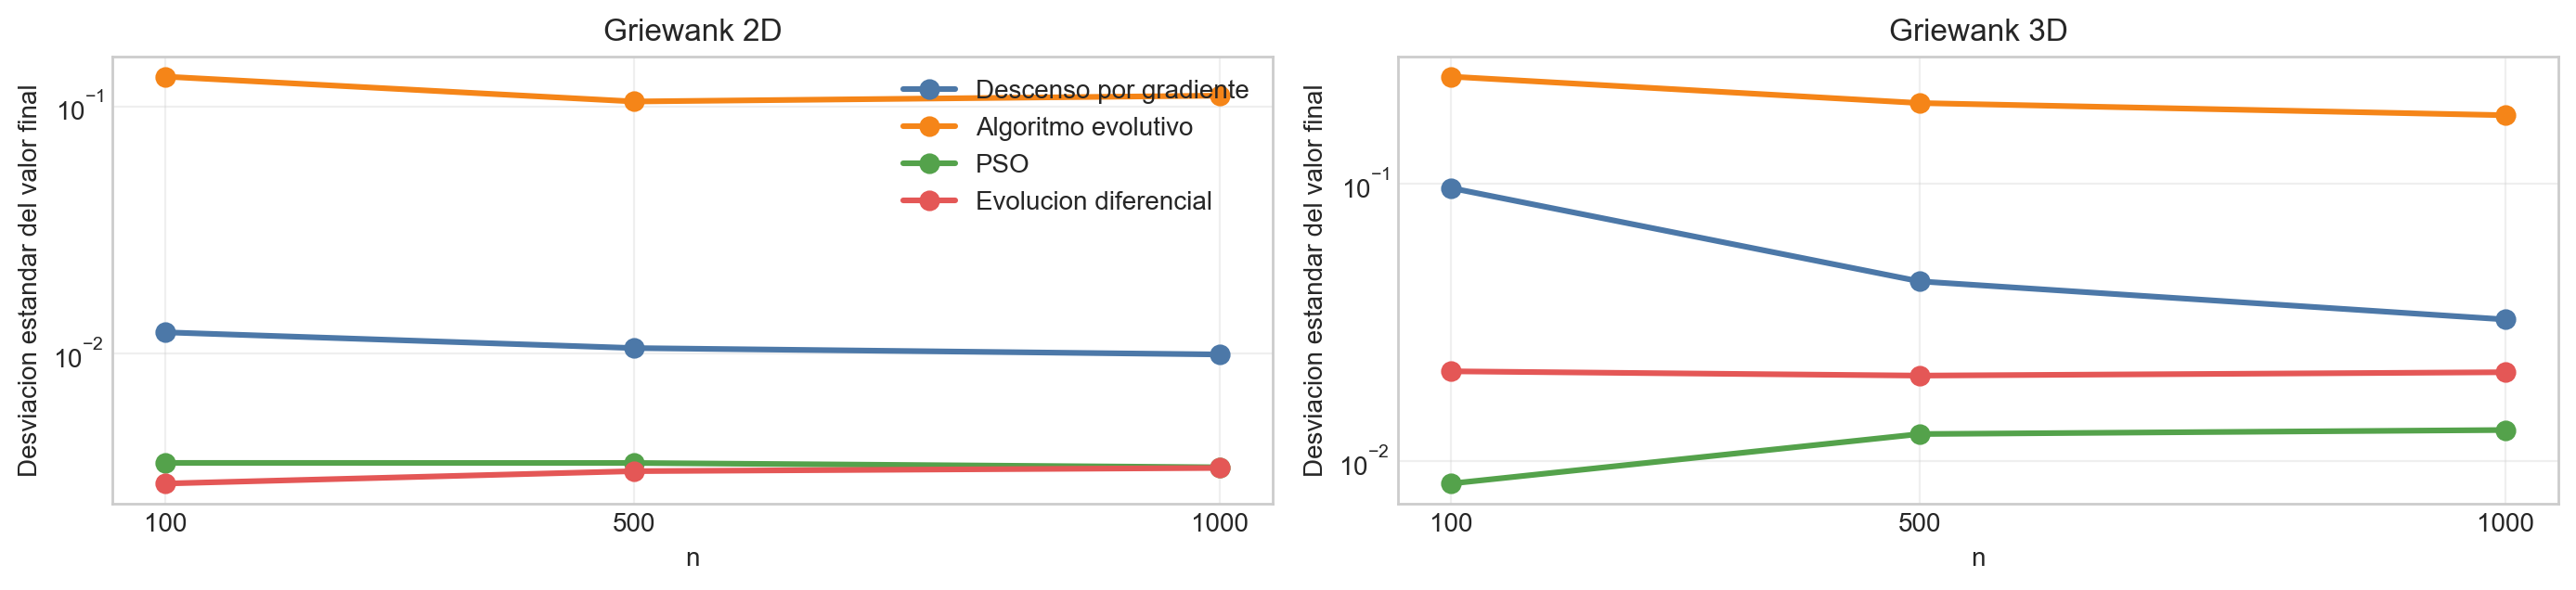
\includegraphics[keepaspectratio]{assets/comparacion/griewank_lineas_desviacion_por_n.png}}
\end{itemize}

En la función Griewank se observa un comportamiento menos uniforme entre
métodos que en los casos anteriores. En 2D,
\texttt{Evolución\ diferencial} logra el mejor resultado, ya que se
mantiene prácticamente sobre el óptimo y con la menor desviación,
mientras que \texttt{PSO} también presenta un desempeño bastante sólido.

En 3D, el método que mejor se comporta es \texttt{PSO}, porque alcanza
los valores medianos más bajos y conserva una variabilidad reducida;
\texttt{Evolución\ diferencial} se mantiene competitivo, aunque ya no
domina con la misma claridad que en 2D.

Por otro lado, el \texttt{Algoritmo\ evolutivo} es el más débil en ambas
dimensiones, al registrar los valores finales más altos y la mayor
dispersión, mientras que \texttt{Descenso\ por\ gradiente} queda en una
posición intermedia.

\begin{itemize}
\tightlist
\item
  \texttt{Goldstein-Price\ 2D}: gradiente vs EA vs PSO vs DE
\end{itemize}

En la función \texttt{Goldstein-Price\ 2D}, \texttt{PSO} y
\texttt{Evolución\ diferencial} muestran el mejor comportamiento, ya que
alcanzan valores finales medianos prácticamente coincidentes con el
óptimo y, además, presentan una variabilidad extremadamente baja. El
\texttt{Algoritmo\ evolutivo} también logra aproximarse bien al valor
óptimo, aunque con una dispersión mayor que estos dos métodos. En
contraste, \texttt{Descenso\ por\ gradiente} es claramente el más débil,
porque se mantiene muy alejado del óptimo y exhibe la mayor desviación,
lo que refleja menor precisión y menor estabilidad.

\begin{itemize}
\tightlist
\item
  \texttt{Six-Hump\ Camel\ 2D}: gradiente vs EA vs PSO vs DE
\end{itemize}

En la función \texttt{Six-Hump\ Camel\ 2D}, \texttt{PSO} y
\texttt{Evolución\ diferencial} son los métodos más precisos, ya que se
mantienen prácticamente sobre el valor óptimo y presentan una dispersión
extremadamente baja. El \texttt{Algoritmo\ evolutivo} también logra
resultados cercanos, aunque sus valores medianos quedan ligeramente por
encima del óptimo y muestran una variabilidad mayor.

Por su parte, \texttt{Descenso\ por\ gradiente} es el enfoque menos
estable, al registrar con diferencia la desviación más alta entre todos
los métodos comparados.

\subsubsection{Tabla comparativa global}\label{tabla-comparativa-global}

{\def\LTcaptype{none} % do not increment counter
\begin{longtable}[]{@{}
  >{\raggedright\arraybackslash}p{(\linewidth - 4\tabcolsep) * \real{0.3333}}
  >{\raggedright\arraybackslash}p{(\linewidth - 4\tabcolsep) * \real{0.3333}}
  >{\raggedright\arraybackslash}p{(\linewidth - 4\tabcolsep) * \real{0.3333}}@{}}
\toprule\noalign{}
\begin{minipage}[b]{\linewidth}\raggedright
Caso
\end{minipage} & \begin{minipage}[b]{\linewidth}\raggedright
Mejor método en valor final o distancia al óptimo
\end{minipage} & \begin{minipage}[b]{\linewidth}\raggedright
Mejor método en evaluaciones
\end{minipage} \\
\midrule\noalign{}
\endhead
\bottomrule\noalign{}
\endlastfoot
Goldstein-Price 2D & Evolución diferencial & Evolución diferencial \\
Griewank 2D & PSO & Descenso por gradiente \\
Griewank 3D & PSO & Descenso por gradiente \\
Rastrigin 2D & Evolución diferencial & Descenso por gradiente \\
Rastrigin 3D & Evolución diferencial & Descenso por gradiente \\
Rosenbrock 2D & Evolución diferencial & Descenso por gradiente \\
Rosenbrock 3D & Evolución diferencial & Descenso por gradiente \\
Schwefel 2D & Evolución diferencial & Evolución diferencial \\
Schwefel 3D & Evolución diferencial & Evolución diferencial \\
Six-Hump Camel 2D & PSO & Descenso por gradiente \\
\end{longtable}
}

\subsubsection{Conteo global de
victorias}\label{conteo-global-de-victorias}

Aquí se presenta un cierre simple contando cuántas veces ganó cada
método.

{\def\LTcaptype{none} % do not increment counter
\begin{longtable}[]{@{}lrr@{}}
\toprule\noalign{}
Método & Veces que ganó en calidad & Veces que ganó en evaluaciones \\
\midrule\noalign{}
\endhead
\bottomrule\noalign{}
\endlastfoot
Gradiente & 0 & 7 \\
EA & 0 & 0 \\
PSO & 3 & 0 \\
DE & 7 & 3 \\
\end{longtable}
}

\subsubsection{Conclusiones}\label{conclusiones}

\paragraph{\texorpdfstring{\textbf{Conclusión 1: Mejor calidad de
solución en los métodos
heurísticos}}{Conclusión 1: Mejor calidad de solución en los métodos heurísticos}}\label{conclusiuxf3n-1-mejor-calidad-de-soluciuxf3n-en-los-muxe9todos-heuruxedsticos}

En términos de calidad de solución, los métodos heurísticos dominaron la
comparación: ganaron en los \texttt{10\ de\ 10} casos analizados. Dentro
de ese grupo, \texttt{Evolución\ diferencial} obtuvo el mejor resultado
en \texttt{7} casos y \texttt{PSO} en \texttt{3}, mientras que
\texttt{Algoritmo\ evolutivo} y \texttt{Descenso\ por\ gradiente} no
lideraron ningún caso en esta métrica.

\paragraph{\texorpdfstring{\textbf{Conclusión 2: Mayor eficiencia
computacional del descenso por
gradiente}}{Conclusión 2: Mayor eficiencia computacional del descenso por gradiente}}\label{conclusiuxf3n-2-mayor-eficiencia-computacional-del-descenso-por-gradiente}

En costo computacional, medido por el número de evaluaciones de la
función objetivo, \texttt{Descenso\ por\ gradiente} fue el método más
eficiente en \texttt{7\ de\ 10} casos. Los \texttt{3} casos restantes
fueron ganados por \texttt{Evolución\ diferencial}, lo que muestra que
gradiente suele ser más barato, aunque no necesariamente el más preciso.

\paragraph{\texorpdfstring{\textbf{Conclusión 3: Aporte comparado entre
descenso por gradiente y métodos
heurísticos}}{Conclusión 3: Aporte comparado entre descenso por gradiente y métodos heurísticos}}\label{conclusiuxf3n-3-aporte-comparado-entre-descenso-por-gradiente-y-muxe9todos-heuruxedsticos}

Los resultados muestran un patrón claro: los métodos heurísticos
aportaron mejor precisión global, mientras que
\texttt{Descenso\ por\ gradiente} aportó mayor rapidez en la mayoría de
los casos. Además, \texttt{Evolución\ diferencial} fue el único método
que logró combinar ambas ventajas en algunos problemas, siendo el mejor
tanto en calidad como en evaluaciones en \texttt{3} casos:
\texttt{Goldstein-Price\ 2D}, \texttt{Schwefel\ 2D} y
\texttt{Schwefel\ 3D}.

\subsubsection{Animación representativa del método
ganador}\label{animaciuxf3n-representativa-del-muxe9todo-ganador}

Como cierre visual de la comparación numérica, se incluye una animación
de \texttt{evolución\ diferencial} sobre la función
\texttt{Rastrigin\ 2D}. Este caso se eligió porque \texttt{DE} fue el
método con mejor desempeño global en la comparación final y porque
\texttt{Rastrigin} presenta una superficie altamente multimodal, con
muchos mínimos locales, lo que permite visualizar con claridad la
capacidad de exploración del algoritmo.

La animación resume de manera intuitiva por qué los métodos heurísticos,
y en particular la evolución diferencial, pueden ofrecer ventajas frente
a un método local cuando el paisaje de optimización es complejo, ya que
fueron diseñados para la optimización global en espacios continuos y
favorecen una exploración más robusta del espacio de búsqueda (Storn and
Price 1997).

\pandocbounded{\includegraphics[keepaspectratio]{assets/histogramas/animacion_de_rastrigin_2d_semilla_1612.gif}}

\subsubsection{Fuente de datos}\label{fuente-de-datos}

Esta comparación debe salir de:

\begin{itemize}
\tightlist
\item
  \href{notebooks/numerica/gradiente/analisis_resultados.ipynb}{analisis\_resultados.ipynb}
\item
  \href{notebooks/numerica/heuristicos/analisis_resultados.ipynb}{analisis\_resultados.ipynb}
\item
  \href{notebooks/numerica/12_comparacion_final_metodos.ipynb}{12\_comparacion\_final\_metodos.ipynb}
\end{itemize}

\section{Parte 2: Optimización Combinatoria (TSP - 96 Departamentos de
Francia)}\label{parte-2-optimizaciuxf3n-combinatoria-tsp---96-departamentos-de-francia}

\subsection{3.1 Descripción del
problema}\label{descripciuxf3n-del-problema}

En la segunda parte del trabajo se aborda una variante del
\textbf{Problema del Viajante (TSP)} aplicada al recorrido de las
\textbf{96 capitales departamentales de Francia metropolitana}. El
objetivo consiste en encontrar un orden de visita para todas las
ciudades tal que se minimice el costo total del recorrido, cumpliendo la
condición clásica del TSP: cada ciudad debe visitarse exactamente una
vez y, al finalizar, se debe completar el circuito regresando al punto
de partida o cerrando la gira definida para la evaluación. Debido a que
el número de rutas posibles crece de forma factorial con respecto al
número de ciudades, se trata de un problema combinatorio de muy alta
complejidad, para el cual resulta poco práctico aplicar métodos exactos
en tiempos razonables (Applegate et al. 2006).

En este contexto, cada solución candidata puede representarse como una
permutación de las 96 ciudades, donde el orden de los elementos define
la ruta seguida por el vendedor. Sin embargo, la evaluación de esa ruta
no se realiza directamente sobre el grafo parcial original, sino sobre
una matriz completa de costos mínimos entre todas las parejas de
ciudades. De esta manera, el problema no se limita a encontrar la ruta
más corta en kilómetros, sino la ruta de \textbf{menor costo total},
incorporando factores operativos más cercanos a una situación real de
desplazamiento y dejando la instancia lista para ser tratada como un TSP
clásico.

La función objetivo utilizada en la implementación combina directamente
tres componentes por tramo: \textbf{peajes}, \textbf{gasolina} y
\textbf{costo del tiempo del vendedor}. En particular, el componente de
combustible no se estima como distancia por costo por kilómetro, sino
que se toma directamente de la columna \texttt{gasolina(euros)}
recuperada del dataset. A esto se suma el costo temporal del vendedor,
calculado a partir del tiempo de viaje y una tarifa fija de
\textbf{12.02 EUR/h}. En forma compacta, la expresión empleada es:

\[
\text{Costo total} = \text{peajes(euros)} + \text{gasolina(euros)} + \left(\frac{\text{tiempo(min)}}{60}\right)\times 12.02
\]

Bajo esta formulación, el costo total de un tour se obtiene acumulando
ese valor sobre los tramos recorridos en la ruta. Esto hace que el
problema sea especialmente adecuado para el uso de metaheurísticas, ya
que el reto consiste en explorar un espacio enorme de posibles
recorridos y encontrar una secuencia que balancee de manera eficiente
tiempo y costo monetario en una red vial real.

\subsection{3.2 Construcción y preprocesamiento de
datos}\label{construcciuxf3n-y-preprocesamiento-de-datos}

La construcción del conjunto de datos para esta parte del trabajo se
realizó en varias etapas. Primero, se extrajeron las coordenadas
geográficas de las ciudades desde el sitio web
\href{https://geokeo.com/database/town/fr/23/}{GeoKeo}, tomando como
referencia las capitales departamentales de Francia. A partir de estas
coordenadas se generó una primera estructura de conexiones entre
ciudades cercanas, utilizada como base para construir un grafo inicial
de rutas, el cual fue exportado a un archivo CSV para facilitar su
revisión posterior.

Posteriormente, este grafo fue ajustado y validado manualmente con apoyo
de visualizaciones sobre mapa, con el fin de identificar conexiones
plausibles dentro de la red y corregir aquellas que no representaban
trayectos razonables. Esta etapa fue importante porque la cercanía
geográfica por sí sola no garantiza que dos ciudades estén conectadas
por una ruta real o conveniente dentro de la red vial.

Una vez consolidada esta red base, se realizó el proceso de
\texttt{web\ scraping} sobre el sitio
\href{https://www.vinci-autoroutes.com/fr/mon-trajet/}{VINCI
Autoroutes}, utilizando las rutas previamente definidas para consultar y
completar información real de los trayectos. En particular, para cada
conexión se obtuvo la distancia recorrida, el tiempo estimado de viaje y
el valor de los peajes. Para mantener consistencia en la recolección de
la información, en VINCI Autoroutes se utilizó la categoría
\textbf{Clase 1 - Vehículos ligeros}, correspondiente a automóviles
particulares y vehículos de uso ligero (VINCI Autoroutes 2026). Estos
datos sirvieron como base para estructurar el conjunto final utilizado
en la optimización combinatoria.

Como paso previo a la optimización, se calculó el costo mínimo de viaje
entre cada par de ciudades a partir de la red de conexiones disponibles.
Para ello se aplicó el algoritmo de Dijkstra, un método clásico para
encontrar caminos de costo mínimo en grafos (Dijkstra 1959). De esta
forma se construyó una matriz completa de costos \texttt{96\ x\ 96}, que
fue la utilizada posteriormente por ACO y GA. Sobre esa matriz se
verificó que la estructura fuera cuadrada, que la diagonal quedara en
cero y que no existieran valores infinitos fuera de la diagonal,
asegurando así una representación consistente del problema.

{ } {Cuaderno de construcción inicial del grafo}

\subsection{3.3 Algoritmos utilizados}\label{algoritmos-utilizados}

Para resolver este problema se emplearon dos metaheurísticas clásicas
para optimización combinatoria: \textbf{Colonia de Hormigas (ACO)} y
\textbf{Algoritmos Genéticos (GA)}. La elección de estos métodos
responde a que ambos están diseñados para explorar espacios de búsqueda
discretos muy grandes y han mostrado buen desempeño en variantes del
TSP. Además, permiten balancear de manera flexible los procesos de
exploración y explotación, lo cual es importante cuando se busca escapar
de soluciones pobres sin perder la capacidad de refinar rutas
prometedoras (Talbi 2009).

\paragraph{Colonia de Hormigas (ACO)}\label{colonia-de-hormigas-aco}

El algoritmo de colonia de hormigas construye soluciones de manera
progresiva, simulando el comportamiento colectivo de hormigas que
depositan feromonas sobre los caminos recorridos. En cada iteración,
varias hormigas generan rutas completas entre las ciudades, eligiendo el
siguiente nodo con base en una combinación entre la \textbf{feromona
acumulada} y una \textbf{heurística local} asociada al inverso del costo
entre ciudades. Con el paso de las iteraciones, las rutas de menor costo
reciben mayor refuerzo y tienden a guiar la búsqueda hacia regiones más
prometedoras del espacio de soluciones.

En la implementación utilizada se fijaron los siguientes parámetros:

\begin{itemize}
\tightlist
\item
  número de hormigas: \texttt{40}
\item
  número de iteraciones: \texttt{250}
\item
  importancia de la feromona (\texttt{alpha}): \texttt{1.0}
\item
  importancia de la heurística (\texttt{beta}): \texttt{3.0}
\item
  tasa de evaporación: \texttt{0.35}
\item
  factor de intensificación: \texttt{2.0}
\item
  peso elitista para reforzar la mejor ruta global: \texttt{2.0}
\item
  semilla aleatoria: \texttt{42}
\end{itemize}

\paragraph{Experimentación con distintas
configuraciones}\label{experimentaciuxf3n-con-distintas-configuraciones}

\begin{itemize}
\tightlist
\item
  Experimento cambiando \texttt{número\ de\ hormigas}:
\end{itemize}

\pandocbounded{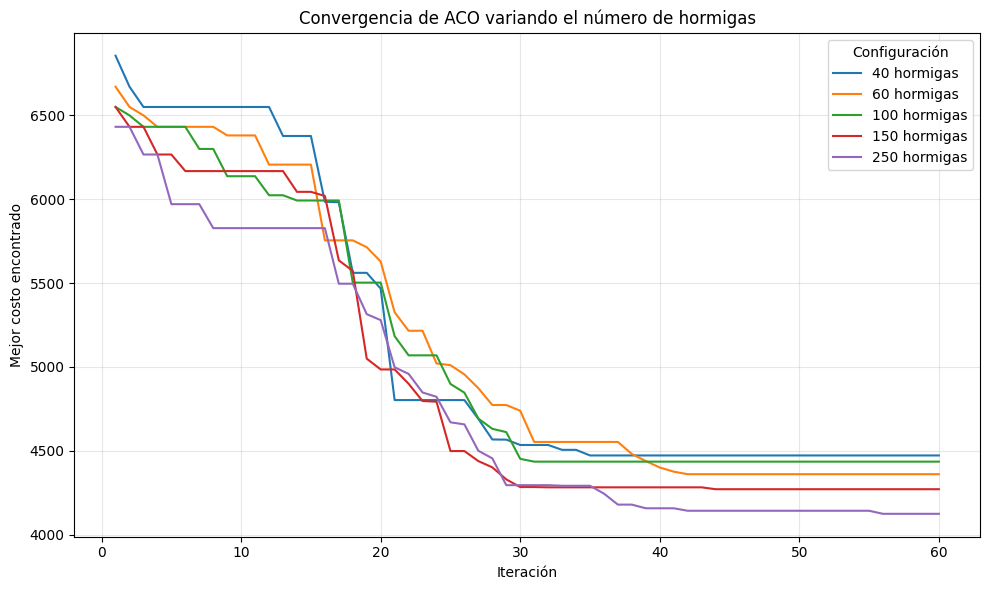
\includegraphics[keepaspectratio]{assets/combinatoria/aco/aco_ants.png}}

La gráfica muestra que todas las configuraciones mejoran con rapidez en
las primeras iteraciones y luego se estabilizan, así que 250 iteraciones
parecen más de las necesarias para este experimento. La mejor
configuración fue la de 80 hormigas, ya que alcanzó el menor costo final
(aprox. 4100), mientras que 20 hormigas obtuvo el peor resultado. En
general, aumentar el número de hormigas parece mejorar la exploración y
permitir mejores soluciones, aunque la mejora no es totalmente uniforme
entre todas las configuraciones. De todos modos, como aquí se usa una
sola semilla, sería recomendable repetir el experimento con varias
corridas y también comparar contra tiempo de ejecución, porque más
hormigas implican mayor costo computacional.

\begin{itemize}
\tightlist
\item
  Experimento cambiando \texttt{beta}:
\end{itemize}

\pandocbounded{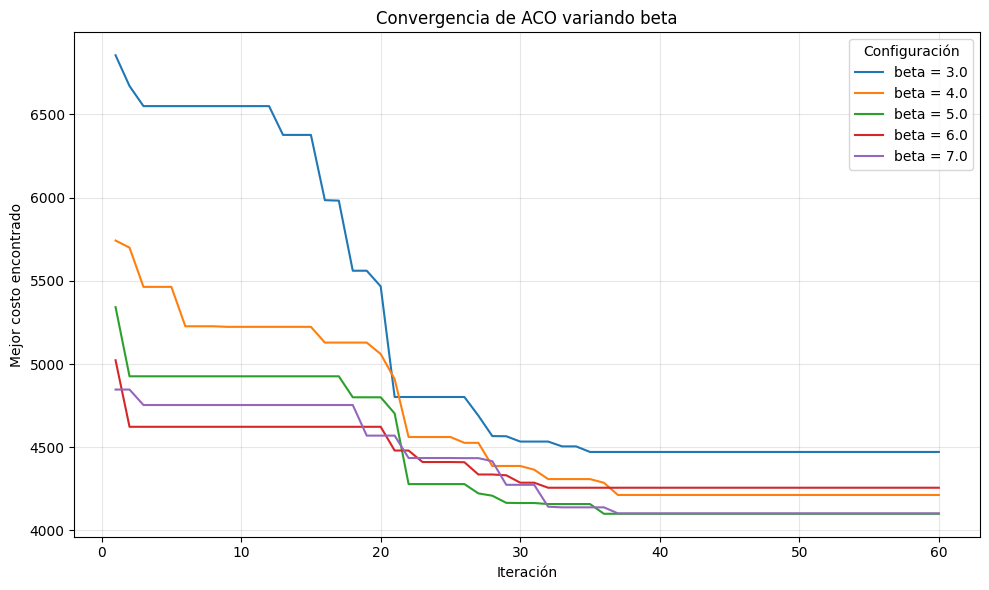
\includegraphics[keepaspectratio]{assets/combinatoria/aco/aco_beta.png}}

Aquí se ve más claro el efecto de \texttt{beta}: cuando \textbf{beta es
bajo (\texttt{3.0})}, el algoritmo converge más lento y además termina
con el \textbf{peor costo final}. En cambio, con valores más altos, la
convergencia mejora bastante y se alcanzan soluciones de mejor calidad.

Las mejores configuraciones parecen ser \textbf{\texttt{beta\ =\ 5.0} y
\texttt{beta\ =\ 7.0}}, que llegan a los \textbf{costos más bajos}
(cerca de 4100), mientras que \textbf{\texttt{beta\ =\ 6.0} y
\texttt{beta\ =\ 4.0}} quedan en un punto intermedio. En general, esto
sugiere que \textbf{dar más peso a la heurística ayuda}, aunque el
efecto no es totalmente lineal, porque no todos los valores altos de
\texttt{beta} rinden igual.

Estos valores permiten dar mayor peso a la información heurística del
costo entre ciudades, sin eliminar la influencia del aprendizaje
colectivo por feromonas. La evaporación evita que la búsqueda se
estanque demasiado pronto en rutas subóptimas, mientras que el refuerzo
elitista ayuda a conservar y explotar la mejor solución global
encontrada hasta cada iteración.

\begin{itemize}
\tightlist
\item
  Experimento cambiando \texttt{evaporation\ rate}:
\end{itemize}

\pandocbounded{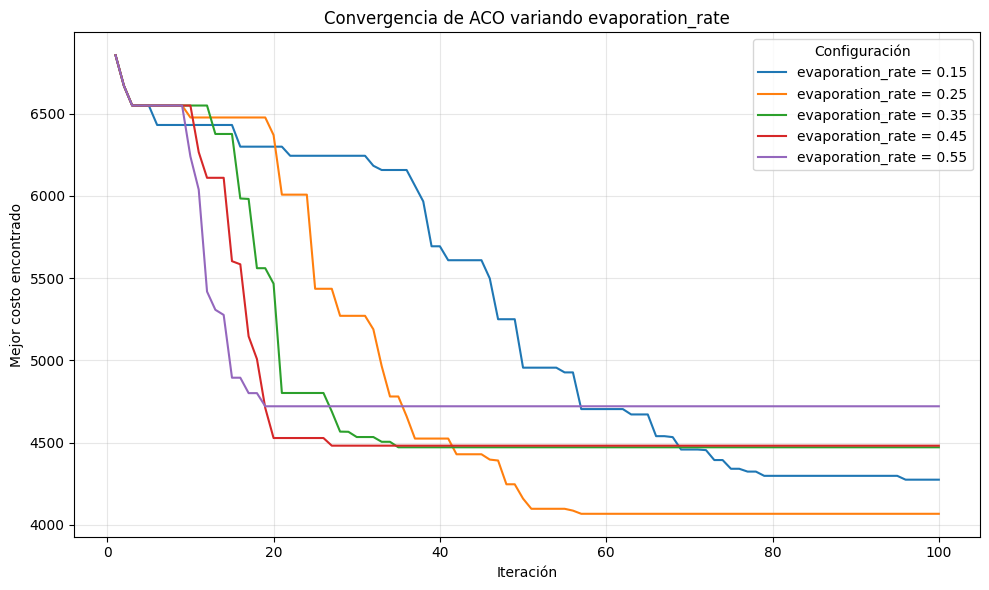
\includegraphics[keepaspectratio]{assets/combinatoria/aco/aco_evaporation_rate.png}}

Aquí se ve que la \textbf{tasa de evaporación sí cambia bastante el
comportamiento} del ACO. Con \textbf{\texttt{0.25}} se obtiene el
\textbf{mejor costo final} (aprox. \textbf{4060}), aunque no es la curva
que baja más rápido al inicio. En cambio, con \textbf{\texttt{0.55}} la
mejora inicial es muy rápida, pero se estanca pronto y termina con el
\textbf{peor resultado final}.

En general, esto sugiere que una evaporación \textbf{intermedia}
funciona mejor: si es \textbf{muy baja} (\texttt{0.15}), el algoritmo
tarda más en adaptarse; si es \textbf{muy alta} (\texttt{0.55}), pierde
demasiado rápido la información acumulada. Por eso, en este experimento,
\textbf{\texttt{0.25} parece el mejor equilibrio entre exploración y
explotación}.

\paragraph{Configuración final de parámetros para el modelo de Colonia
de
Hormigas}\label{configuraciuxf3n-final-de-paruxe1metros-para-el-modelo-de-colonia-de-hormigas}

De acuerdo con los experimentos realizados, se estableció la siguiente
configuración para el algoritmo de colonia de hormigas (ACO), buscando
un equilibrio entre la exploración del espacio de soluciones y la
explotación de las mejores rutas encontradas:

\begin{itemize}
\tightlist
\item
  número de hormigas: \texttt{150}
\item
  número de iteraciones: \texttt{100}
\item
  importancia de la feromona (\texttt{alpha}): \texttt{1.0}
\item
  importancia de la heurística (\texttt{beta}): \texttt{5.0}
\item
  tasa de evaporación: \texttt{0.25}
\item
  factor de intensificación: \texttt{2.0}
\item
  peso elitista para reforzar la mejor ruta global: \texttt{2.0}
\item
  semilla aleatoria: \texttt{no\ especificada}
\end{itemize}

\subsubsection{Algoritmos Genéticos
(GA)}\label{algoritmos-genuxe9ticos-ga}

El algoritmo genético aborda el problema manteniendo una
\textbf{población de rutas candidatas} que evoluciona a lo largo de
varias generaciones. Cada individuo representa un recorrido completo por
las ciudades, y su aptitud se evalúa con el costo total de la ruta. A
partir de esta evaluación, se seleccionan las mejores soluciones para
producir descendencia mediante operadores de cruce y mutación. De este
modo, el método combina información de rutas de buena calidad y genera
nuevas alternativas que pueden mejorar progresivamente el resultado
obtenido.

En este trabajo, el GA se implementó con una estrategia de
\textbf{selección por torneo}, \textbf{cruce ordenado} y
\textbf{mutación por intercambio} de posiciones dentro de la ruta.
Además, se permitió inyectar como semilla inicial la mejor ruta
producida por ACO, con el fin de aprovechar una buena solución de
partida y refinarla en una fase evolutiva posterior.

Los parámetros iniciales usados fueron:

\begin{itemize}
\tightlist
\item
  tamaño de población: \texttt{180}
\item
  número de generaciones: \texttt{350}
\item
  tasa de mutación: \texttt{0.12}
\item
  tasa de cruce: \texttt{0.9}
\item
  número de individuos elitistas preservados por generación: \texttt{12}
\item
  tamaño del torneo de selección: \texttt{5}
\item
  uso de semilla inicial proveniente de ACO: \texttt{True}
\item
  semilla aleatoria: \texttt{42}
\end{itemize}

La justificación de esta configuración es que una población
relativamente amplia favorece la diversidad de soluciones, mientras que
una tasa de cruce alta promueve la recombinación de rutas prometedoras.
La mutación moderada introduce variación sin destruir excesivamente las
estructuras útiles encontradas, y el elitismo garantiza que las mejores
soluciones no se pierdan entre generaciones.

\paragraph{Experimentación con distintas
configuraciones}\label{experimentaciuxf3n-con-distintas-configuraciones-1}

\begin{itemize}
\tightlist
\item
  Experimento cambiando \texttt{tasa\ de\ mutación}:
\end{itemize}

\pandocbounded{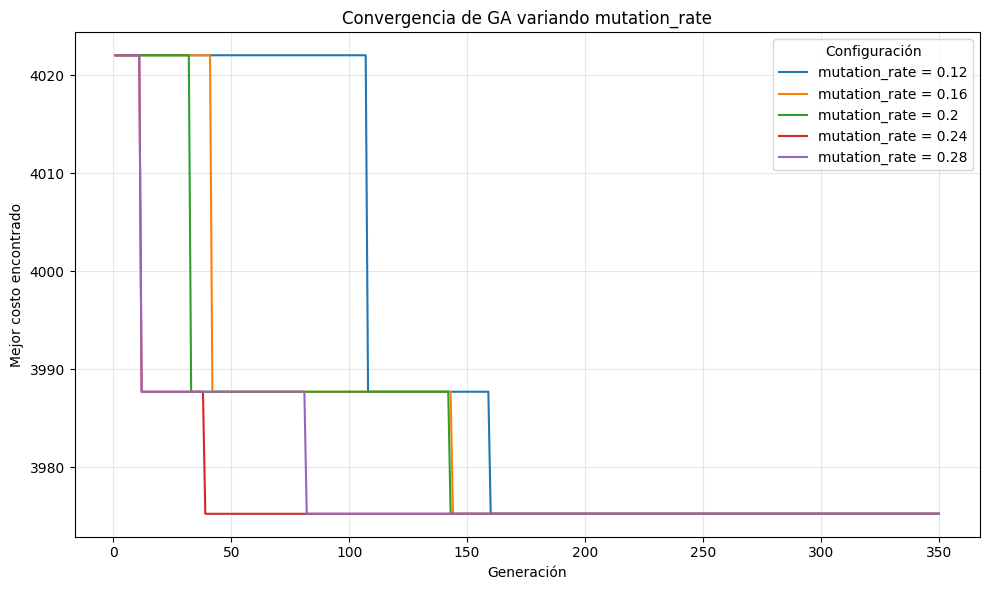
\includegraphics[keepaspectratio]{assets/combinatoria/ga/ga_mutation_rate.png}}

Aquí se ve que \textbf{todas las tasas de mutación terminan llegando
prácticamente al mismo costo final} (cerca de \textbf{3975}), así que en
este experimento la diferencia no está tanto en la calidad final sino en
la \textbf{velocidad de convergencia}. La más lenta es
\textbf{\texttt{mutation\_rate\ =\ 0.12}}, mientras que
\textbf{\texttt{0.24} y \texttt{0.28}} encuentran mejoras antes.

En general, esto sugiere que una \textbf{mutación moderadamente alta
ayuda a acelerar la búsqueda} sin perjudicar el resultado final. Si
tuvieras que escoger una opción balanceada,
\textbf{\texttt{mutation\_rate\ =\ 0.24}} se ve como una muy buena
candidata, porque converge rápido sin irse al valor más extremo.

\begin{itemize}
\tightlist
\item
  Experimento cambiando \texttt{tamaño\ de\ población}:
\end{itemize}

\pandocbounded{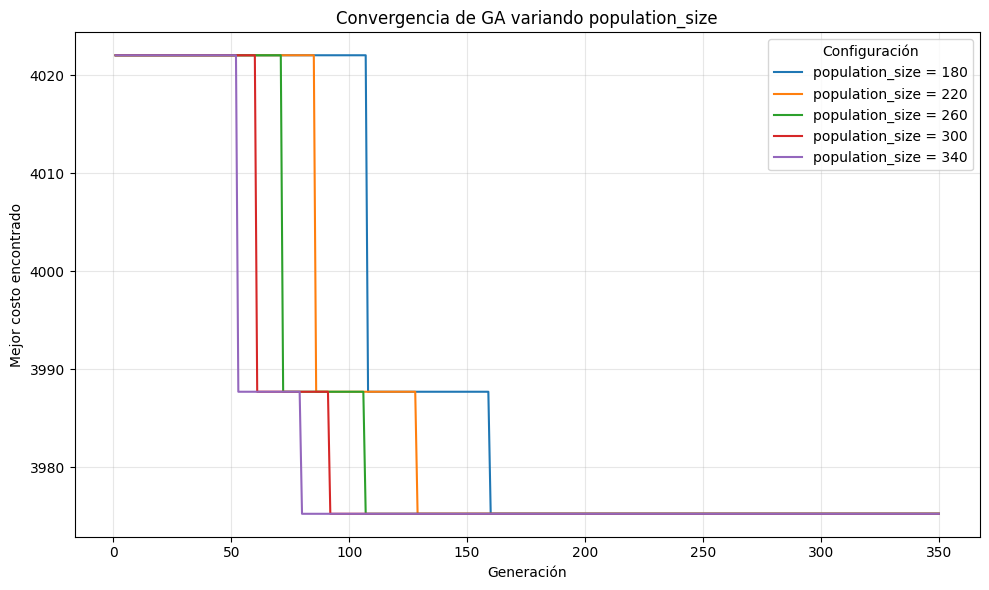
\includegraphics[keepaspectratio]{assets/combinatoria/ga/ga_population_rate.png}}

Aquí se ve que tamaños de población más grandes convergen más rápido:
340 y 300 encuentran mejoras antes, mientras que 180 es claramente la
más lenta. Sin embargo, todas terminan llegando prácticamente al mismo
costo final (cerca de 3975), así que la diferencia principal está en la
rapidez, no en la calidad final.

Eso sugiere que aumentar population\_size ayuda a acelerar la búsqueda,
pero con rendimientos decrecientes. Como además una población más grande
cuesta más por generación, no necesariamente conviene irse al valor
máximo. Si buscas una opción balanceada, population\_size = 260 o 300 se
ven como candidatas razonables.

\begin{itemize}
\tightlist
\item
  Experimento cambiando
  \texttt{uso\ de\ semilla\ inicial\ proveniente\ de\ ACO}:
\end{itemize}

\pandocbounded{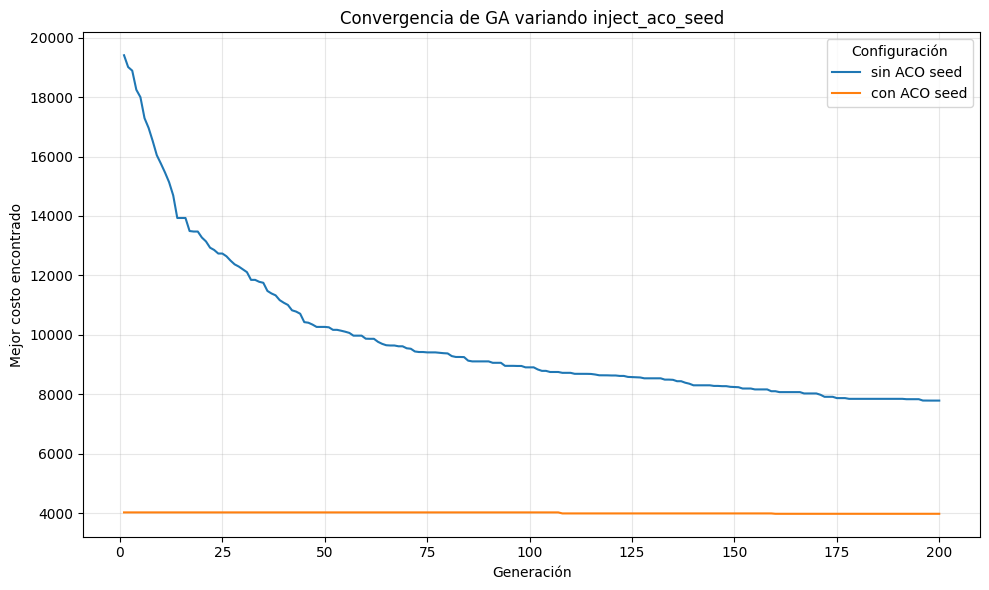
\includegraphics[keepaspectratio]{assets/combinatoria/ga/ga_aco_seed.png}}

Aquí la diferencia es muy marcada: usar ACO seed hace que el GA arranque
desde un costo mucho mejor, cerca de 4000, mientras que sin ACO seed
empieza alrededor de 19400 y, aunque mejora de forma sostenida, después
de 200 generaciones todavía queda muy por encima.

Esto sugiere que inyectar la solución de ACO es altamente beneficioso,
porque acelera muchísimo la convergencia y además lleva al algoritmo a
una región de soluciones mucho mejores desde el inicio. De hecho, con
ACO seed casi no hay mejoras adicionales, lo que indica que ACO ya
entrega una solución inicial muy fuerte y el GA solo la refina
ligeramente.

\subsection{Configuración final de parámetros para el algoritmo
genético}\label{configuraciuxf3n-final-de-paruxe1metros-para-el-algoritmo-genuxe9tico}

De acuerdo con los experimentos realizados, se estableció la siguiente
configuración para el algoritmo genético (GA), buscando un equilibrio
entre diversidad poblacional, intensidad de búsqueda y preservación de
las mejores soluciones encontradas:

\begin{itemize}
\tightlist
\item
  tamaño de población: \texttt{300}
\item
  número de generaciones: \texttt{200}
\item
  tasa de mutación: \texttt{0.24}
\item
  tasa de cruce: \texttt{0.9}
\item
  número de individuos elitistas preservados por generación: \texttt{12}
\item
  tamaño del torneo de selección: \texttt{5}
\item
  uso de semilla inicial proveniente de ACO: \texttt{True}
\item
  semilla aleatoria: \texttt{42}
\end{itemize}

\subsection{3.4 Resultados}\label{resultados}

Los experimentos realizados sobre la instancia de las 96 capitales
departamentales muestran que ambos métodos fueron capaces de producir
recorridos válidos y de costo competitivo. Sin embargo, el mejor
resultado final fue alcanzado por el \textbf{algoritmo genético (GA)},
que logró refinar la solución inicial y obtener un costo total inferior
al conseguido por la colonia de hormigas.

La comparación final entre métodos puede resumirse en la siguiente
tabla:

{\def\LTcaptype{none} % do not increment counter
\begin{longtable}[]{@{}
  >{\raggedright\arraybackslash}p{(\linewidth - 8\tabcolsep) * \real{0.1579}}
  >{\raggedleft\arraybackslash}p{(\linewidth - 8\tabcolsep) * \real{0.2105}}
  >{\raggedleft\arraybackslash}p{(\linewidth - 8\tabcolsep) * \real{0.2105}}
  >{\raggedleft\arraybackslash}p{(\linewidth - 8\tabcolsep) * \real{0.2105}}
  >{\raggedleft\arraybackslash}p{(\linewidth - 8\tabcolsep) * \real{0.2105}}@{}}
\toprule\noalign{}
\begin{minipage}[b]{\linewidth}\raggedright
Método
\end{minipage} & \begin{minipage}[b]{\linewidth}\raggedleft
Mejor costo del tour (EUR)
\end{minipage} & \begin{minipage}[b]{\linewidth}\raggedleft
Diferencia frente al mejor (EUR)
\end{minipage} & \begin{minipage}[b]{\linewidth}\raggedleft
Iteraciones / generaciones
\end{minipage} & \begin{minipage}[b]{\linewidth}\raggedleft
Tamaño de búsqueda
\end{minipage} \\
\midrule\noalign{}
\endhead
\bottomrule\noalign{}
\endlastfoot
GA & 3975.266333 & 0.000000 & 350 & 300 \\
ACO & 4022.039333 & 46.773000 & 250 & 150 \\
\end{longtable}
}

El \textbf{mejor costo encontrado} fue de \textbf{3975.266333 euros},
calculado con la función de costo definida a partir de peajes,
combustible y tiempo del vendedor. Este resultado se obtuvo usando como
vehículo de referencia un \textbf{Renault Clio}, con combustible tipo
gasolina, y una tarifa del vendedor de \textbf{12.02 euros por hora}, de
acuerdo con la formulación del modelo. Además, aunque el tour TSP
recorre las \textbf{96 capitales}, su expansión sobre el grafo real
produce un recorrido de \textbf{100 saltos reales}, lo que permite
interpretar la solución final de manera más fiel a la red de conexiones
utilizada.

En cuanto a la comparación entre métodos, ACO alcanzó un mejor costo de
\textbf{4022.039333 euros}, mientras que GA obtuvo \textbf{3975.266333
euros}. En otras palabras, \textbf{GA mejoró a ACO en 46.773000 euros,
equivalente a una mejora relativa de 1.1629 \%}. Esta diferencia es
menor que en versiones preliminares de los experimentos, lo que indica
que ambos métodos terminaron convergiendo a soluciones de alta calidad y
muy cercanas entre sí.

Desde el punto de vista de la convergencia, esta dinámica resulta
especialmente interesante. ACO encuentra con rapidez una solución base
competitiva para una instancia grande del TSP, mientras que GA, apoyado
en una población más amplia y en la inyección de la mejor solución
previa de ACO, consigue seguir refinando la ruta hasta obtener la mejor
solución final. En este sentido, los resultados no solo muestran
competencia entre ambos enfoques, sino también una
\textbf{complementariedad efectiva} dentro del flujo de optimización.

La \textbf{mejor ruta encontrada} puede resumirse por tramos geográficos
de la siguiente forma:

\begin{itemize}
\tightlist
\item
  corredor este y noreste:
  \texttt{Bourg-en-Bresse\ -\textgreater{}\ Lons-le-Saunier\ -\textgreater{}\ Besançon\ -\textgreater{}\ Vesoul\ -\textgreater{}\ Belfort\ -\textgreater{}\ Colmar\ -\textgreater{}\ Strasbourg\ -\textgreater{}\ Metz\ -\textgreater{}\ Nancy\ -\textgreater{}\ Épinal\ -\textgreater{}\ Chaumont\ -\textgreater{}\ Dijon\ -\textgreater{}\ Auxerre\ -\textgreater{}\ Troyes\ -\textgreater{}\ Bar-le-Duc\ -\textgreater{}\ Châlons-en-Champagne\ -\textgreater{}\ Charleville-Mézières\ -\textgreater{}\ Laon}
\item
  norte y eje parisino:
  \texttt{Lille\ -\textgreater{}\ Arras\ -\textgreater{}\ Amiens\ -\textgreater{}\ Beauvais\ -\textgreater{}\ Cergy\ -\textgreater{}\ Nanterre\ -\textgreater{}\ Bobigny\ -\textgreater{}\ Créteil\ -\textgreater{}\ Paris\ -\textgreater{}\ Versailles\ -\textgreater{}\ Évry-Courcouronnes\ -\textgreater{}\ Melun}
\item
  centro-oeste y fachada atlántica:
  \texttt{Orléans\ -\textgreater{}\ Blois\ -\textgreater{}\ Tours\ -\textgreater{}\ Poitiers\ -\textgreater{}\ Niort\ -\textgreater{}\ La\ Rochelle\ -\textgreater{}\ La\ Roche-sur-Yon\ -\textgreater{}\ Nantes\ -\textgreater{}\ Vannes\ -\textgreater{}\ Quimper\ -\textgreater{}\ Saint-Brieuc\ -\textgreater{}\ Rennes\ -\textgreater{}\ Laval\ -\textgreater{}\ Angers\ -\textgreater{}\ Le\ Mans\ -\textgreater{}\ Alençon\ -\textgreater{}\ Caen\ -\textgreater{}\ Saint-Lô\ -\textgreater{}\ Rouen\ -\textgreater{}\ Évreux\ -\textgreater{}\ Chartres\ -\textgreater{}\ Bourges\ -\textgreater{}\ Châteauroux\ -\textgreater{}\ Guéret\ -\textgreater{}\ Limoges\ -\textgreater{}\ Tulle\ -\textgreater{}\ Aurillac}
\item
  suroccidente y arco mediterráneo:
  \texttt{Rodez\ -\textgreater{}\ Albi\ -\textgreater{}\ Montauban\ -\textgreater{}\ Cahors\ -\textgreater{}\ Agen\ -\textgreater{}\ Périgueux\ -\textgreater{}\ Angoulême\ -\textgreater{}\ Bordeaux\ -\textgreater{}\ Mont-de-Marsan\ -\textgreater{}\ Pau\ -\textgreater{}\ Tarbes\ -\textgreater{}\ Auch\ -\textgreater{}\ Toulouse\ -\textgreater{}\ Foix\ -\textgreater{}\ Carcassonne\ -\textgreater{}\ Perpignan\ -\textgreater{}\ Montpellier\ -\textgreater{}\ Nîmes\ -\textgreater{}\ Avignon\ -\textgreater{}\ Marseille\ -\textgreater{}\ Toulon\ -\textgreater{}\ Bastia\ -\textgreater{}\ Ajaccio\ -\textgreater{}\ Nice\ -\textgreater{}\ Digne-les-Bains\ -\textgreater{}\ Gap}
\item
  retorno alpino y centro-este:
  \texttt{Grenoble\ -\textgreater{}\ Valence\ -\textgreater{}\ Privas\ -\textgreater{}\ Mende\ -\textgreater{}\ Le\ Puy-en-Velay\ -\textgreater{}\ Saint-Étienne\ -\textgreater{}\ Clermont-Ferrand\ -\textgreater{}\ Moulins\ -\textgreater{}\ Nevers\ -\textgreater{}\ Mâcon\ -\textgreater{}\ Lyon\ -\textgreater{}\ Chambéry\ -\textgreater{}\ Annecy\ -\textgreater{}\ Bourg-en-Bresse}
\end{itemize}

En términos cualitativos, los resultados muestran una dinámica
complementaria entre ambos enfoques. ACO aporta una exploración guiada
por información local y memoria colectiva, lo que permite encontrar
rápidamente rutas razonables en un espacio de búsqueda muy grande. Por
su parte, GA aprovecha esa base inicial y la mejora mediante operadores
evolutivos, conservando buenas estructuras parciales y corrigiendo
tramos menos eficientes del recorrido. Por esta razón, dentro de los
experimentos realizados, \textbf{GA puede considerarse el método con
mejor desempeño final} para esta instancia del problema, aunque la
brecha observada frente a ACO sugiere que ambos métodos fueron altamente
competitivos.

\subsection{3.5 Visualización}\label{visualizaciuxf3n}

La visualización final se realiza sobre el mapa de \textbf{Francia},
mostrando el recorrido ganador obtenido por el algoritmo genético. El
GIF permite observar la progresión espacial del tour, mientras que la
curva de convergencia muestra cómo el costo va disminuyendo a medida que
avanzan las generaciones del método ganador.

\subsubsection{Comparación visual de
costos}\label{comparaciuxf3n-visual-de-costos}

\subsubsection{GIF del mejor recorrido en
Francia}\label{gif-del-mejor-recorrido-en-francia}

\subsubsection{Curva de convergencia del método
ganador}\label{curva-de-convergencia-del-muxe9todo-ganador}

Como apoyo adicional, también se dispone de una visualización estática
del tour ganador, útil para inspeccionar la forma general del recorrido
sin necesidad de reproducir la animación.

\section{Conclusiones y Aprendizajes}\label{conclusiones-y-aprendizajes}

\subsection{Conclusiones generales}\label{conclusiones-generales}

El trabajo permitió comparar dos familias de problemas de optimización
con naturalezas muy distintas y dejó una conclusión central: la elección
del método depende directamente de la estructura del problema. En la
parte de optimización numérica, el descenso por gradiente mostró un buen
comportamiento cuando la geometría de la función favorecía el uso de
información local, como ocurrió especialmente en \texttt{Griewank},
\texttt{Six-Hump\ Camel} y, en menor medida, \texttt{Rosenbrock\ 2D}.
Sin embargo, en funciones altamente multimodales o con paisajes más
irregulares, como \texttt{Rastrigin}, \texttt{Schwefel} y
\texttt{Goldstein-Price}, su desempeño se deterioró por la sensibilidad
al punto inicial y la facilidad con la que puede quedar atrapado en
mínimos locales.

La comparación final de la parte numérica confirmó que los métodos
heurísticos ofrecieron la mejor calidad de solución en todos los casos
analizados. Dentro de ellos, \texttt{Evolución\ diferencial} fue el
método más robusto a nivel global, con el mejor resultado en
\texttt{7\ de\ 10} casos, mientras que \texttt{PSO} destacó
especialmente en \texttt{Griewank} y \texttt{Six-Hump\ Camel}. Aun así,
el descenso por gradiente conservó una ventaja importante en eficiencia
computacional, ya que fue el método con menor número de evaluaciones en
\texttt{7\ de\ 10} casos. Esto muestra un patrón claro: los métodos
locales pueden ser más baratos, pero los heurísticos y metaheurísticos
son mucho más sólidos cuando la dificultad del paisaje aumenta.

En la parte de optimización combinatoria, el TSP sobre las \texttt{96}
capitales departamentales de Francia evidenció que, en espacios
discretos de gran tamaño, los enfoques exactos dejan de ser prácticos y
las metaheurísticas se convierten en la alternativa más razonable. Tanto
\texttt{ACO} como \texttt{GA} encontraron recorridos competitivos, pero
el algoritmo genético alcanzó el mejor costo final con
\texttt{3975.266333} euros, superando a \texttt{ACO}, que obtuvo
\texttt{4022.039333} euros. La mejora fue de \texttt{46.773000} euros,
equivalente a \texttt{1.1629\ \%}, lo que confirma que ambos métodos
fueron competitivos, pero que \texttt{GA} tuvo una mayor capacidad de
refinamiento sobre la solución final.

Un hallazgo especialmente valioso fue la complementariedad entre
métodos. En la parte combinatoria, \texttt{ACO} mostró una muy buena
capacidad para construir rápidamente una solución inicial de alta
calidad, mientras que \texttt{GA} resultó más fuerte en la fase de
mejora fina. Esta lógica de exploración seguida de refinamiento resume
uno de los aprendizajes más importantes del proyecto: en problemas
complejos, combinar estrategias puede ser más efectivo que depender de
un único enfoque desde el inicio.

\subsection{Aprendizajes
metodológicos}\label{aprendizajes-metodoluxf3gicos}

Otro resultado transversal del trabajo es que el éxito de la
optimización no depende solo del algoritmo, sino también de cómo se
formula el problema. En la parte combinatoria, la construcción del
grafo, el \texttt{web\ scraping} de trayectos reales y la generación de
una matriz completa de costos mínimos mediante \texttt{Dijkstra} fueron
pasos tan importantes como la elección de \texttt{ACO} o \texttt{GA}. De
forma análoga, en la parte numérica, la interpretación de la geometría
de cada función fue clave para entender por qué algunos métodos
convergían con estabilidad y otros no.

En conjunto, el proyecto confirma que no existe un método universalmente
superior para todos los escenarios. Los métodos clásicos, como el
descenso por gradiente, son apropiados cuando la función es
diferenciable, el paisaje es relativamente favorable y se busca una
solución rápida con bajo costo computacional. En cambio, los métodos
heurísticos y metaheurísticos son preferibles cuando el problema es
multimodal, la dimensión crece, el espacio de búsqueda es discreto o la
información local ya no basta para orientar la búsqueda.

Como conclusión final, el trabajo muestra que optimizar no consiste en
aplicar siempre el mismo algoritmo, sino en seleccionar o combinar
herramientas según la dificultad, la representación y los objetivos del
problema. Esa fue la lección más importante tanto en la parte numérica
como en la combinatoria: la calidad de la solución depende de la
correspondencia entre el método elegido y la naturaleza real del
problema que se quiere resolver.

\section{Parte 4: Uso de Inteligencia Artificial en el
Proyecto}\label{parte-4-uso-de-inteligencia-artificial-en-el-proyecto}

\subsection{4.1 Prompts principales
utilizados}\label{prompts-principales-utilizados}

Los prompts reportados en esta seccion son una reconstruccion fiel de
los usos principales que tuvo la IA durante el proyecto. No buscan ser
una transcripcion literal de cada chat, sino resumir de forma clara las
solicitudes que realmente influyeron en la implementacion, el analisis
de resultados y la presentacion final del trabajo.

\subsubsection{Prompt 1: diseno de experimentos para ACO y
GA}\label{prompt-1-diseno-de-experimentos-para-aco-y-ga}

\begin{Shaded}
\begin{Highlighting}[]
\NormalTok{Estoy comparando colonia de hormigas y algoritmo genetico para el TSP de las capitales departamentales de Francia. Ayudame a decidir que hiperparametros vale la pena experimentar en cada metodo y a escribir el codigo para correr esos barridos, guardar resultados y graficar la convergencia.}
\end{Highlighting}
\end{Shaded}

\textbf{Impacto en el resultado final.} Este tipo de prompt permitio
estructurar de manera mas rapida los experimentos de
\texttt{mutation\_rate}, \texttt{population\_size} e
\texttt{inject\_aco\_seed} en \texttt{GA}, y de \texttt{ants},
\texttt{beta} y \texttt{evaporation\_rate} en \texttt{ACO}. Gracias a
ello se pudieron comparar configuraciones reales en vez de dejar la
seleccion de parametros a prueba y error informal.

\subsubsection{Prompt 2: interpretacion de curvas y seleccion de
configuracion
final}\label{prompt-2-interpretacion-de-curvas-y-seleccion-de-configuracion-final}

\begin{Shaded}
\begin{Highlighting}[]
\NormalTok{Ya tengo las graficas y tablas de los experimentos de ACO y GA. Ayudame a interpretarlas y a escoger una configuracion balanceada, explicando que parametros mejoran el costo final, cuales aceleran la convergencia y cuales solo aumentan el costo computacional.}
\end{Highlighting}
\end{Shaded}

\textbf{Impacto en el resultado final.} La IA se uso como apoyo para
leer las curvas de convergencia y justificar mejor la eleccion final de
configuraciones. En particular, ayudo a identificar el efecto positivo
de \texttt{inject\_aco\_seed}, el papel de \texttt{mutation\_rate} en la
velocidad de refinamiento de \texttt{GA} y el compromiso entre calidad y
costo computacional en \texttt{ACO}.

\subsubsection{Prompt 3: visualizacion de la mejor ruta sobre el mapa de
Francia}\label{prompt-3-visualizacion-de-la-mejor-ruta-sobre-el-mapa-de-francia}

\begin{Shaded}
\begin{Highlighting}[]
\NormalTok{Quiero mostrar la mejor ruta final sobre un mapa de Francia dentro del notebook y no solo como un SVG estilizado. Ayudame a construir una visualizacion con folium o plotly, exportarla para el reporte y dejarla lista para incrustarla junto con la curva de convergencia.}
\end{Highlighting}
\end{Shaded}

\textbf{Impacto en el resultado final.} Este prompt mejoro de forma
directa la calidad de la presentacion. La mejor solucion ya no quedo
solo como una polilinea abstracta, sino como una ruta visible sobre un
mapa, lo que hace mucho mas clara la interpretacion geografica del
recorrido final y fortalece la calidad del reporte.

\subsubsection{Prompt 4: integracion de tablas, figuras y texto en el
reporte
tecnico}\label{prompt-4-integracion-de-tablas-figuras-y-texto-en-el-reporte-tecnico}

\begin{Shaded}
\begin{Highlighting}[]
\NormalTok{Ayudame a convertir los resultados de los notebooks en una seccion de reporte tecnico en Quarto. Quiero una tabla comparativa final entre metodos, una explicacion breve de la convergencia y una redaccion clara de los hallazgos mas importantes.}
\end{Highlighting}
\end{Shaded}

\textbf{Impacto en el resultado final.} La IA ayudo a pasar de
resultados dispersos en notebooks a una narrativa tecnica mas ordenada.
Esto facilito integrar tablas, figuras y conclusiones en un formato
consistente para el informe final, especialmente en la comparacion entre
metodos y en la lectura de la convergencia.

\subsubsection{Prompt 5: organizacion e interpretacion de resultados en
optimizacion
numerica}\label{prompt-5-organizacion-e-interpretacion-de-resultados-en-optimizacion-numerica}

\begin{Shaded}
\begin{Highlighting}[]
\NormalTok{Necesito resumir los resultados de descenso por gradiente y de los metodos heuristicos en tablas y figuras comparables. Ayudame a insertar las tablas reales, escoger visualizaciones utiles e interpretar que se observa en terminos de calidad de solucion, estabilidad y numero de evaluaciones.}
\end{Highlighting}
\end{Shaded}

\textbf{Impacto en el resultado final.} Este tipo de prompt sirvio para
mejorar la lectura comparativa en la parte numerica. La IA ayudo a
seleccionar que figuras eran mas utiles, como presentar los histogramas
y como traducir los resultados cuantitativos en una discusion mas clara
sobre robustez, multimodalidad y costo computacional.

\subsubsection{Prompt 6: redaccion de introducciones, metodologia y
cierre}\label{prompt-6-redaccion-de-introducciones-metodologia-y-cierre}

\begin{Shaded}
\begin{Highlighting}[]
\NormalTok{Ayudame a redactar una introduccion breve, la metodologia y las conclusiones de un reporte academico sobre optimizacion numerica y combinatoria, manteniendo un tono tecnico y conectando bien los resultados con la discusion final.}
\end{Highlighting}
\end{Shaded}

\textbf{Impacto en el resultado final.} La IA se uso como apoyo de
escritura tecnica para ordenar el documento y reducir tiempo de
redaccion. Esto no sustituyo el analisis propio, pero si ayudo a que el
informe final tuviera una estructura mas coherente y una mejor
transicion entre problema, metodologia, resultados y conclusiones.

\subsection{4.2 Impacto global de la IA en el
proyecto}\label{impacto-global-de-la-ia-en-el-proyecto}

En conjunto, la IA tuvo cuatro aportes principales dentro del trabajo.
Primero, acelero la implementacion y depuracion de codigo para
experimentos y visualizaciones. Segundo, ayudo a disenar mejor los
barridos de parametros y a interpretar las curvas de convergencia, lo
que tuvo impacto directo en la seleccion de configuraciones para
\texttt{ACO} y \texttt{GA}. Tercero, mejoro la presentacion de
resultados, especialmente en la ruta final sobre el mapa y en la
organizacion de tablas y figuras. Cuarto, sirvio como apoyo para
estructurar el reporte tecnico y redactar secciones de forma mas clara.

Por tanto, el uso de IA no consistio en delegar automaticamente la
solucion del trabajo, sino en utilizarla como herramienta de apoyo para
programacion, analisis y escritura tecnica. Las decisiones finales, la
ejecucion de los experimentos, la seleccion de configuraciones y la
revision del contenido quedaron bajo control del desarrollo realizado en
el proyecto.

\protect\phantomsection\label{refs}
\begin{CSLReferences}{1}{1}
\bibitem[\citeproctext]{ref-applegate2006}
Applegate, David L., Robert E. Bixby, Vasek Chvatal, and William J.
Cook. 2006. \emph{The Traveling Salesman Problem: A Computational
Study}. Princeton University Press.

\bibitem[\citeproctext]{ref-dijkstra1959}
Dijkstra, E. W. 1959. {``A Note on Two Problems in Connexion with
Graphs.''} \emph{Numerische Mathematik} 1: 269--71.
\url{https://doi.org/10.1007/BF01386390}.

\bibitem[\citeproctext]{ref-jamil2013}
Jamil, Momin, and Xin-She Yang. 2013. {``A Literature Survey of
Benchmark Functions for Global Optimisation Problems.''}
\emph{International Journal of Mathematical Modelling and Numerical
Optimisation} 4 (2): 150--94.
\url{https://doi.org/10.1504/IJMMNO.2013.055204}.

\bibitem[\citeproctext]{ref-nocedal2006}
Nocedal, Jorge, and Stephen J. Wright. 2006. \emph{Numerical
Optimization}. 2nd ed. Springer.
\url{https://doi.org/10.1007/978-0-387-40065-5}.

\bibitem[\citeproctext]{ref-storn1997}
Storn, Rainer, and Kenneth Price. 1997. {``Differential Evolution -- a
Simple and Efficient Heuristic for Global Optimization over Continuous
Spaces.''} \emph{Journal of Global Optimization} 11 (4): 341--59.
\url{https://doi.org/10.1023/A:1008202821328}.

\bibitem[\citeproctext]{ref-talbi2009}
Talbi, El-Ghazali. 2009. \emph{Metaheuristics: From Design to
Implementation}. John Wiley \& Sons.
\url{https://doi.org/10.1002/9780470496916}.

\bibitem[\citeproctext]{ref-vinci2026}
VINCI Autoroutes. 2026. \emph{Mon Trajet}.
\url{https://www.vinci-autoroutes.com/fr/mon-trajet/}.

\end{CSLReferences}




\end{document}
